\clearpage
\thispagestyle{empty}
\null
\newpage

\cleardoublepage
\phantomsection
% \pdfbookmark[1]{The MAMAD method}{The MAMAD method}
\markboth{\spacedlowsmallcaps{The MAMAD method}}{\spacedlowsmallcaps{The MAMAD method}}
\part{The MAMAD method}
\label{part:method}

\clearpage
\thispagestyle{empty}
\null
\newpage

% todo: Initially, in Part I, our problem was one of designing software for a Cyberdefense \acn{SMA} capable of providing optimal cyberdefense given the dynamic constraints of the environment and the designers. We formalized the fact that to answer this overall research question, six criteria must be met simultaneously (Autonomy - C1, Performance - C2, Adaptation - C3, Control - C4, Explainability - C5, Robustness - C6) . We therefore conducted an initial literature review, which showed us that relatively little work has been done on a multi-agent approach to cyber defense and that the work covering the most criteria can be found in the connectionist approach, which favors performance and adaptation, whereas the purely symbolic approach favors explainability and control. Based on this observation, we proposed to view the overall research question through the prism of a constrained optimization problem where the joint policy is to be optimized to maximize a reward that encodes success in achieving a cyber defense objective (or a conglomerate of objectives) and where the constraints are formalized as organizational specifications. Based on this formalization, the complexity of the overall research question appears to be manageable through four activities: Modeling, Training, Analysis, and Transfer. For each activity, we know the input data, the expected output data, and therefore also the objectives of each activity.
Based on this vision, section \acn{II} presents the work covering the objectives for each activity, thus identifying the areas/sub-areas or work that seem most appropriate (or that require the least additional input) to achieve the objectives of each activity. Given the work identified as most promising, we can deduce the gaps that still need to be filled by new contributions in order to achieve the objectives of each activity.
Part \acn{III} presents the method that orchestrates the four activities and explains how we have overcome the obstacles in each activity with new contributions. In this part, we first give a general presentation of the method that orchestrates the four activities. We then detail each activity, briefly reviewing the objectives and each of the associated obstacles, and for each one we detail our contribution and justify it. Once this is done, we provide an algorithmic representation of the activity, which serves as a basis for formally detailing the activity by explaining each of the formal elements (set, element of a set, relation, etc.). At the end of the activity, we provide a summary, explaining what we think will be covered in terms of expected objectives, what is covered moderately and why, and what is not covered at all.
% Part \acn{IV} concerns the experimental validation of the method by applying it to three non-cyberdefense-oriented case studies and three cyberdefense-oriented case studies. The objective is to verify that the six criteria (Autonomy - C1, Performance - C2, Adaptation - C3, Control - C4, Explainability - C5) are well covered. To do this, we apply an evaluation grid that associates each criterion with a set of measurable metrics that can be analyzed to see whether the criterion is covered or not. As the reading grid is common to all six environments, we can therefore verify in a more consistent and generic way whether the method does indeed cover the six criteria. The section therefore concludes with an overall analysis of whether the method adequately covers the six criteria initially set out.

% \acn{TODO}:
% - Overall, harmonize the vocabulary
% - Overall, correctly introduce technical/theoretical terms such as “organizational adequacy,” “\acn{RNN},” “\acn{VAE},” “\acn{LSTM},” and “World Models,” in particular to enable readers unfamiliar with \acn{ML} or \acn{AI} in general to understand.
% - In the chapters on “Modeling,” “Training,” “Analysis,” and “Transfer,” care must be taken to clearly explain the objectives of each activity, the assumptions that define our research space in the literature, the work most likely to achieve the objectives of the activity (e.g., Constrained-\acn{RL}, Shielding, etc.), and the associated obstacles that remain to be overcome (e.g., the lack of means to guide learning with an organizational model) through new contributions. Next, we present these different contributions (e.g., the MOISE+MARL framework). Then, we can present the activity in the form of an algorithm that articulates the identified work and/or contributions to meet the objectives of the activity. Care must be taken to explain this algorithm in detail (referencing each of the formal elements of the algorithm) to provide as complete a description of the activity as possible. Finally, we must explain why we believe that this implementation of the activity does or does not meet the objectives of the activity. Further on, we can even say whether we believe that the criteria associated with an activity are well covered by the current implementation of the activity.

\chapter*{Introduction}
\addcontentsline{toc}{chapter}{\textbf{Introduction}}

\noindent

The previous section highlighted the current shortcomings in the integration of organizational models within multi-agent learning approaches, in terms of control, explainability, and design automation. It also highlighted gaps in environment modeling and its integration into the training process, particularly the lack of a framework to ensure consistency between the simulated and real environments.

\medskip

\noindent
This third section presents our proposal to address these gaps: the \acn{MAMAD}\index{MAMAD} method. This method is based on the premise that the design of an \acn{SMA} can be approached through the prism of a constrained optimization problem. The method is built around this vision and is organized around four activities:

\begin{enumerate}
  \item \textbf{Modeling}: modeling the real environment in a simulated environment as well as design constraints in organizational specifications;
  \item \textbf{Learning}: training agents in this simulated environment, taking into account organizational specifications such as roles during learning;
  \item \textbf{Analysis}: extracting emerging structural and functional specifications from the trajectories of trained agents;
  \item \textbf{Transfer}: regularly updating the policies of agents deployed in the real environment based on the policies of agents trained in simulation and, if necessary, updating or improving the simulated environment.
\end{enumerate}

\noindent
These four activities can be seen as performed iteratively to produce \acplu{SMA}s that are adapted to their environment, aligned with organizational constraints, explainable, and robust.

\medskip

\noindent
\autoref{chap:mamad_global} provides an overview of the method concerning the proposed processes. The remaining four chapters detail each of the steps in this method:
\autoref{chap:modeling} presents the modeling activity.
\autoref{chap:training} presents the learning activity constrained by organizational specifications.
\autoref{chap:analyzing} presents a method for analyzing trajectories to infer emerging organizational structures.
\autoref{chap:transferring} describes the transfer activity.
\autoref{fig:organisation_manuscript_part_3} illustrates the organization of this part.

The \acn{MAMAD} method aims to combine the strengths of symbolic and connectionist approaches for a structured, autonomous, and explainable \acn{SMA} design.

\begin{figure}[h!]
  \centering
  \resizebox{0.7\linewidth}{!}{%
    \input{figures/organization_manuscript_part_3}
  }
  \caption{Structure of Part III: The MAMAD method}
  \label{fig:organization_manuscript_part_3}
\end{figure}



\clearpage
\thispagestyle{empty}
\null
\newpage

\chapter{Overall presentation of the method}
\label{chap:mamad_global}

The \acn{MAMAD} method~\footnotemark[2] is based on four main activities: (1) modeling the environment, the overall objective, and organizational constraints, (2) learning policies using various \acn{MARL} algorithms, (3) analyzing behaviors and inferring organizational specifications using a proposed method, and (4) maintaining consistency between the simulated environment and the real environment by deploying the trained policies and updating the simulation. This approach guides the agent learning process while imposing strict organizational constraints, thus ensuring the effectiveness of the learned policies.

The life cycle of an \acn{SMA} designed with \acn{MAMAD} is illustrated in \autoref{fig:cycle}. It begins with the modeling of the environment, based on a sufficient set of real trajectories (from already transferred agents or any other available source), as well as the definition of the overall objective and design constraints in the form of roles and goals. Next, the agents are trained in this simulated environment using \acn{MARL} (\acn{MARL}) techniques. Once training is complete, a post-training analysis extracts the emerging roles and objectives of the agents, leading to improvements in the applied organizational specifications. Finally, after validation, the learned policies are deployed to control the environment's actuators, generating new traces that will be used to refine the modeling in subsequent iterations.

\begin{figure}[h!]
  \centering
  


\tikzset{every picture/.style={line width=0.75pt}} %set default line width to 0.75pt        

\begin{tikzpicture}[x=0.75pt,y=0.75pt,yscale=-1,xscale=1]
%uncomment if require: \path (0,3307); %set diagram left start at 0, and has height of 3307

%Shape: Smiley Face [id:dp29065495216725257] 
\draw  [line width=1.5]  (85.38,2800.11) .. controls (85.38,2797.7) and (87.16,2795.75) .. (89.36,2795.75) .. controls (91.55,2795.75) and (93.34,2797.7) .. (93.34,2800.11) .. controls (93.34,2802.52) and (91.55,2804.48) .. (89.36,2804.48) .. controls (87.16,2804.48) and (85.38,2802.52) .. (85.38,2800.11) -- cycle ; \draw  [line width=1.5]  (87.61,2798.63) .. controls (87.61,2798.39) and (87.78,2798.19) .. (88,2798.19) .. controls (88.22,2798.19) and (88.4,2798.39) .. (88.4,2798.63) .. controls (88.4,2798.87) and (88.22,2799.07) .. (88,2799.07) .. controls (87.78,2799.07) and (87.61,2798.87) .. (87.61,2798.63) -- cycle ; \draw  [line width=1.5]  (90.31,2798.63) .. controls (90.31,2798.39) and (90.49,2798.19) .. (90.71,2798.19) .. controls (90.93,2798.19) and (91.11,2798.39) .. (91.11,2798.63) .. controls (91.11,2798.87) and (90.93,2799.07) .. (90.71,2799.07) .. controls (90.49,2799.07) and (90.31,2798.87) .. (90.31,2798.63) -- cycle ; \draw  [line width=1.5]  (87.37,2801.86) .. controls (88.69,2803.02) and (90.02,2803.02) .. (91.35,2801.86) ;
%Shape: Rectangle [id:dp42672371521059915] 
\draw  [dash pattern={on 5.63pt off 4.5pt}][line width=1.5]  (74.03,2763.75) -- (192,2763.75) -- (192,2813.93) -- (74.03,2813.93) -- cycle ;
%Shape: Smiley Face [id:dp9817389082285293] 
\draw  [line width=1.5]  (144.45,2803.6) .. controls (144.45,2801.19) and (146.24,2799.24) .. (148.43,2799.24) .. controls (150.63,2799.24) and (152.41,2801.19) .. (152.41,2803.6) .. controls (152.41,2806.01) and (150.63,2807.97) .. (148.43,2807.97) .. controls (146.24,2807.97) and (144.45,2806.01) .. (144.45,2803.6) -- cycle ; \draw  [line width=1.5]  (146.68,2802.12) .. controls (146.68,2801.88) and (146.86,2801.68) .. (147.08,2801.68) .. controls (147.3,2801.68) and (147.48,2801.88) .. (147.48,2802.12) .. controls (147.48,2802.36) and (147.3,2802.56) .. (147.08,2802.56) .. controls (146.86,2802.56) and (146.68,2802.36) .. (146.68,2802.12) -- cycle ; \draw  [line width=1.5]  (149.39,2802.12) .. controls (149.39,2801.88) and (149.57,2801.68) .. (149.79,2801.68) .. controls (150.01,2801.68) and (150.18,2801.88) .. (150.18,2802.12) .. controls (150.18,2802.36) and (150.01,2802.56) .. (149.79,2802.56) .. controls (149.57,2802.56) and (149.39,2802.36) .. (149.39,2802.12) -- cycle ; \draw  [line width=1.5]  (146.44,2805.35) .. controls (147.77,2806.51) and (149.1,2806.51) .. (150.42,2805.35) ;
%Shape: Smiley Face [id:dp49419175504212776] 
\draw  [line width=1.5]  (179.09,2781.5) .. controls (179.09,2779.09) and (180.87,2777.13) .. (183.06,2777.13) .. controls (185.26,2777.13) and (187.04,2779.09) .. (187.04,2781.5) .. controls (187.04,2783.91) and (185.26,2785.86) .. (183.06,2785.86) .. controls (180.87,2785.86) and (179.09,2783.91) .. (179.09,2781.5) -- cycle ; \draw  [line width=1.5]  (181.31,2780.01) .. controls (181.31,2779.77) and (181.49,2779.58) .. (181.71,2779.58) .. controls (181.93,2779.58) and (182.11,2779.77) .. (182.11,2780.01) .. controls (182.11,2780.25) and (181.93,2780.45) .. (181.71,2780.45) .. controls (181.49,2780.45) and (181.31,2780.25) .. (181.31,2780.01) -- cycle ; \draw  [line width=1.5]  (184.02,2780.01) .. controls (184.02,2779.77) and (184.2,2779.58) .. (184.42,2779.58) .. controls (184.64,2779.58) and (184.81,2779.77) .. (184.81,2780.01) .. controls (184.81,2780.25) and (184.64,2780.45) .. (184.42,2780.45) .. controls (184.2,2780.45) and (184.02,2780.25) .. (184.02,2780.01) -- cycle ; \draw  [line width=1.5]  (181.07,2783.24) .. controls (182.4,2784.4) and (183.73,2784.4) .. (185.05,2783.24) ;
%Flowchart: Punched Tape [id:dp3565745198144521] 
\draw  [fill={rgb, 255:red, 255; green, 255; blue, 255 }  ,fill opacity=1 ] (291.67,2877.34) .. controls (291.67,2880.23) and (301.36,2882.58) .. (313.31,2882.58) .. controls (325.26,2882.58) and (334.95,2880.23) .. (334.95,2877.34) .. controls (334.95,2874.45) and (344.64,2872.11) .. (356.6,2872.11) .. controls (368.55,2872.11) and (378.24,2874.45) .. (378.24,2877.34) -- (378.24,2919.23) .. controls (378.24,2916.34) and (368.55,2913.99) .. (356.6,2913.99) .. controls (344.64,2913.99) and (334.95,2916.34) .. (334.95,2919.23) .. controls (334.95,2922.12) and (325.26,2924.46) .. (313.31,2924.46) .. controls (301.36,2924.46) and (291.67,2922.12) .. (291.67,2919.23) -- cycle ;
%Straight Lines [id:da23451091058783402] 
\draw [line width=1.5]    (320.63,2891.89) -- (349.47,2889.91) ;
\draw [shift={(352.46,2889.7)}, rotate = 176.08] [color={rgb, 255:red, 0; green, 0; blue, 0 }  ][line width=1.5]    (8.53,-2.57) .. controls (5.42,-1.09) and (2.58,-0.23) .. (0,0) .. controls (2.58,0.23) and (5.42,1.09) .. (8.53,2.57)   ;
%Straight Lines [id:da05993633349010663] 
\draw [line width=1.5]    (320.63,2894.07) -- (335.84,2901.48) ;
\draw [shift={(338.53,2902.79)}, rotate = 205.98] [color={rgb, 255:red, 0; green, 0; blue, 0 }  ][line width=1.5]    (8.53,-2.57) .. controls (5.42,-1.09) and (2.58,-0.23) .. (0,0) .. controls (2.58,0.23) and (5.42,1.09) .. (8.53,2.57)   ;
%Shape: Smiley Face [id:dp5316832937595011] 
\draw  [line width=1.5]  (312.91,2893.34) .. controls (312.91,2890.93) and (314.69,2888.98) .. (316.89,2888.98) .. controls (319.09,2888.98) and (320.87,2890.93) .. (320.87,2893.34) .. controls (320.87,2895.75) and (319.09,2897.7) .. (316.89,2897.7) .. controls (314.69,2897.7) and (312.91,2895.75) .. (312.91,2893.34) -- cycle ; \draw  [line width=1.5]  (315.14,2891.86) .. controls (315.14,2891.61) and (315.32,2891.42) .. (315.54,2891.42) .. controls (315.76,2891.42) and (315.94,2891.61) .. (315.94,2891.86) .. controls (315.94,2892.1) and (315.76,2892.29) .. (315.54,2892.29) .. controls (315.32,2892.29) and (315.14,2892.1) .. (315.14,2891.86) -- cycle ; \draw  [line width=1.5]  (317.85,2891.86) .. controls (317.85,2891.61) and (318.02,2891.42) .. (318.24,2891.42) .. controls (318.46,2891.42) and (318.64,2891.61) .. (318.64,2891.86) .. controls (318.64,2892.1) and (318.46,2892.29) .. (318.24,2892.29) .. controls (318.02,2892.29) and (317.85,2892.1) .. (317.85,2891.86) -- cycle ; \draw  [line width=1.5]  (314.9,2895.08) .. controls (316.23,2896.25) and (317.55,2896.25) .. (318.88,2895.08) ;
%Shape: Smiley Face [id:dp5491508300746957] 
\draw  [line width=1.5]  (338.38,2904.97) .. controls (338.38,2902.56) and (340.16,2900.61) .. (342.35,2900.61) .. controls (344.55,2900.61) and (346.33,2902.56) .. (346.33,2904.97) .. controls (346.33,2907.38) and (344.55,2909.34) .. (342.35,2909.34) .. controls (340.16,2909.34) and (338.38,2907.38) .. (338.38,2904.97) -- cycle ; \draw  [line width=1.5]  (340.6,2903.49) .. controls (340.6,2903.25) and (340.78,2903.05) .. (341,2903.05) .. controls (341.22,2903.05) and (341.4,2903.25) .. (341.4,2903.49) .. controls (341.4,2903.73) and (341.22,2903.93) .. (341,2903.93) .. controls (340.78,2903.93) and (340.6,2903.73) .. (340.6,2903.49) -- cycle ; \draw  [line width=1.5]  (343.31,2903.49) .. controls (343.31,2903.25) and (343.49,2903.05) .. (343.71,2903.05) .. controls (343.93,2903.05) and (344.1,2903.25) .. (344.1,2903.49) .. controls (344.1,2903.73) and (343.93,2903.93) .. (343.71,2903.93) .. controls (343.49,2903.93) and (343.31,2903.73) .. (343.31,2903.49) -- cycle ; \draw  [line width=1.5]  (340.36,2906.72) .. controls (341.69,2907.88) and (343.02,2907.88) .. (344.34,2906.72) ;
%Shape: Smiley Face [id:dp21362593128550156] 
\draw  [line width=1.5]  (352.64,2888.69) .. controls (352.64,2886.28) and (354.42,2884.32) .. (356.61,2884.32) .. controls (358.81,2884.32) and (360.59,2886.28) .. (360.59,2888.69) .. controls (360.59,2891.1) and (358.81,2893.05) .. (356.61,2893.05) .. controls (354.42,2893.05) and (352.64,2891.1) .. (352.64,2888.69) -- cycle ; \draw  [line width=1.5]  (354.86,2887.2) .. controls (354.86,2886.96) and (355.04,2886.77) .. (355.26,2886.77) .. controls (355.48,2886.77) and (355.66,2886.96) .. (355.66,2887.2) .. controls (355.66,2887.44) and (355.48,2887.64) .. (355.26,2887.64) .. controls (355.04,2887.64) and (354.86,2887.44) .. (354.86,2887.2) -- cycle ; \draw  [line width=1.5]  (357.57,2887.2) .. controls (357.57,2886.96) and (357.75,2886.77) .. (357.97,2886.77) .. controls (358.19,2886.77) and (358.36,2886.96) .. (358.36,2887.2) .. controls (358.36,2887.44) and (358.19,2887.64) .. (357.97,2887.64) .. controls (357.75,2887.64) and (357.57,2887.44) .. (357.57,2887.2) -- cycle ; \draw  [line width=1.5]  (354.62,2890.43) .. controls (355.95,2891.59) and (357.28,2891.59) .. (358.6,2890.43) ;
%Left Arrow [id:dp22187584774212898] 
\draw   (215,2804.55) -- (220.28,2802) -- (220.28,2803.27) -- (263.54,2803.27) -- (263.54,2805.82) -- (220.28,2805.82) -- (220.28,2807.09) -- cycle ;
%Left Arrow [id:dp1861077704673879] 
\draw   (315.35,2834) -- (317.89,2837.8) -- (316.62,2837.8) -- (316.62,2868.91) -- (314.07,2868.91) -- (314.07,2837.8) -- (312.8,2837.8) -- cycle ;
%Left Arrow [id:dp2590948740182193] 
\draw   (130.55,2868.91) -- (128,2865.11) -- (129.27,2865.11) -- (129.27,2834) -- (131.82,2834) -- (131.82,2865.11) -- (133.09,2865.11) -- cycle ;
%Left Arrow [id:dp7631269314674067] 
\draw   (262.54,2900.55) -- (257.26,2903.09) -- (257.26,2901.82) -- (214,2901.82) -- (214,2899.27) -- (257.26,2899.27) -- (257.26,2898) -- cycle ;
%Shape: Arc [id:dp8010751146858193] 
\draw  [draw opacity=0] (78.55,2898.86) .. controls (77.97,2897.43) and (79.7,2895.07) .. (82.41,2893.59) .. controls (85.13,2892.11) and (87.81,2892.08) .. (88.39,2893.51) -- (83.47,2896.19) -- cycle ; \draw   (78.55,2898.86) .. controls (77.97,2897.43) and (79.7,2895.07) .. (82.41,2893.59) .. controls (85.13,2892.11) and (87.81,2892.08) .. (88.39,2893.51) ;  
%Shape: Arc [id:dp2168479262754166] 
\draw  [draw opacity=0] (79.96,2900.21) .. controls (79.37,2898.78) and (80.79,2896.59) .. (83.12,2895.32) .. controls (85.45,2894.06) and (87.81,2894.19) .. (88.39,2895.63) -- (84.17,2897.92) -- cycle ; \draw   (79.96,2900.21) .. controls (79.37,2898.78) and (80.79,2896.59) .. (83.12,2895.32) .. controls (85.45,2894.06) and (87.81,2894.19) .. (88.39,2895.63) ;  
%Shape: Arc [id:dp1657064934185728] 
\draw  [draw opacity=0] (81.36,2901.56) .. controls (81.36,2901.56) and (81.36,2901.56) .. (81.36,2901.56) .. controls (80.78,2900.13) and (81.88,2898.11) .. (83.82,2897.06) .. controls (85.76,2896) and (87.81,2896.31) .. (88.39,2897.74) -- (84.88,2899.65) -- cycle ; \draw   (81.36,2901.56) .. controls (81.36,2901.56) and (81.36,2901.56) .. (81.36,2901.56) .. controls (80.78,2900.13) and (81.88,2898.11) .. (83.82,2897.06) .. controls (85.76,2896) and (87.81,2896.31) .. (88.39,2897.74) ;  
%Shape: Arc [id:dp6696163073703636] 
\draw  [draw opacity=0] (82.77,2902.92) .. controls (82.77,2902.92) and (82.77,2902.92) .. (82.77,2902.92) .. controls (82.77,2902.92) and (82.77,2902.92) .. (82.77,2902.92) .. controls (82.19,2901.48) and (82.97,2899.63) .. (84.53,2898.79) .. controls (86.08,2897.94) and (87.81,2898.42) .. (88.39,2899.86) -- (85.58,2901.39) -- cycle ; \draw   (82.77,2902.92) .. controls (82.77,2902.92) and (82.77,2902.92) .. (82.77,2902.92) .. controls (82.77,2902.92) and (82.77,2902.92) .. (82.77,2902.92) .. controls (82.19,2901.48) and (82.97,2899.63) .. (84.53,2898.79) .. controls (86.08,2897.94) and (87.81,2898.42) .. (88.39,2899.86) ;  
%Shape: Arc [id:dp5914598807756752] 
\draw  [draw opacity=0] (84.18,2904.27) .. controls (83.6,2902.83) and (84.07,2901.15) .. (85.23,2900.52) .. controls (86.4,2899.89) and (87.81,2900.54) .. (88.4,2901.97) -- (86.29,2903.12) -- cycle ; \draw   (84.18,2904.27) .. controls (83.6,2902.83) and (84.07,2901.15) .. (85.23,2900.52) .. controls (86.4,2899.89) and (87.81,2900.54) .. (88.4,2901.97) ;  

%Image [id:dp3722282424817167] 
\draw (291.67,2795.75) node  {
\includegraphics[width=7.64pt,height=13.09pt]{figures/robot.png}};
%Shape: Rectangle [id:dp9197785817800539] 
\draw  [line width=1.5]  (275.37,2763.75) -- (390.8,2763.75) -- (390.8,2813.93) -- (275.37,2813.93) -- cycle ;
%Image [id:dp9715658782589778] 
\draw (382.32,2779.46) node  {
\includegraphics[width=7.64pt,height=13.09pt]{figures/robot.png}};
%Image [id:dp635616861971029] 
\draw (352.78,2801.57) node  {
\includegraphics[width=7.64pt,height=13.09pt]{figures/robot.png}};
%Shape: Rectangle [id:dp647928357040308] 
\draw  [fill={rgb, 255:red, 0; green, 0; blue, 0 }  ,fill opacity=1 ] (291.67,2769.57) -- (301.85,2769.57) -- (301.85,2781.21) -- (291.67,2781.21) -- cycle ;
%Shape: Rectangle [id:dp9626828362725837] 
\draw  [fill={rgb, 255:red, 0; green, 0; blue, 0 }  ,fill opacity=1 ] (373.15,2792.84) -- (383.33,2792.84) -- (383.33,2804.48) -- (373.15,2804.48) -- cycle ;
%Shape: Ellipse [id:dp6171740062199291] 
\draw  [fill={rgb, 255:red, 0; green, 0; blue, 0 }  ,fill opacity=1 ] (347.69,2775.39) .. controls (347.69,2772.17) and (349.97,2769.57) .. (352.78,2769.57) .. controls (355.59,2769.57) and (357.87,2772.17) .. (357.87,2775.39) .. controls (357.87,2778.6) and (355.59,2781.21) .. (352.78,2781.21) .. controls (349.97,2781.21) and (347.69,2778.6) .. (347.69,2775.39) -- cycle ;
%Shape: Triangle [id:dp8145134127966778] 
\draw  [fill={rgb, 255:red, 0; green, 0; blue, 0 }  ,fill opacity=1 ] (322.22,2792.84) -- (327.31,2804.48) -- (317.13,2804.48) -- cycle ;
%Shape: Rectangle [id:dp07981685971419106] 
\draw  [fill={rgb, 255:red, 0; green, 0; blue, 0 }  ,fill opacity=1 ] (89.45,2769.57) -- (99.64,2769.57) -- (99.64,2781.21) -- (89.45,2781.21) -- cycle ;
%Shape: Rectangle [id:dp9786998324005067] 
\draw  [fill={rgb, 255:red, 0; green, 0; blue, 0 }  ,fill opacity=1 ] (170.94,2792.84) -- (181.12,2792.84) -- (181.12,2804.48) -- (170.94,2804.48) -- cycle ;
%Shape: Ellipse [id:dp6465785854464419] 
\draw  [fill={rgb, 255:red, 0; green, 0; blue, 0 }  ,fill opacity=1 ] (145.47,2775.39) .. controls (145.47,2772.17) and (147.75,2769.57) .. (150.57,2769.57) .. controls (153.38,2769.57) and (155.66,2772.17) .. (155.66,2775.39) .. controls (155.66,2778.6) and (153.38,2781.21) .. (150.57,2781.21) .. controls (147.75,2781.21) and (145.47,2778.6) .. (145.47,2775.39) -- cycle ;
%Shape: Triangle [id:dp5909890868954251] 
\draw  [fill={rgb, 255:red, 0; green, 0; blue, 0 }  ,fill opacity=1 ] (120.01,2792.84) -- (125.1,2804.48) -- (114.92,2804.48) -- cycle ;
%Shape: Smiley Face [id:dp661163164093121] 
\draw  [line width=1.5]  (85.52,2909.38) .. controls (85.52,2906.98) and (87.3,2905.03) .. (89.5,2905.03) .. controls (91.7,2905.03) and (93.48,2906.98) .. (93.48,2909.38) .. controls (93.48,2911.78) and (91.7,2913.73) .. (89.5,2913.73) .. controls (87.3,2913.73) and (85.52,2911.78) .. (85.52,2909.38) -- cycle ; \draw  [line width=1.5]  (87.75,2907.9) .. controls (87.75,2907.66) and (87.93,2907.46) .. (88.15,2907.46) .. controls (88.37,2907.46) and (88.55,2907.66) .. (88.55,2907.9) .. controls (88.55,2908.14) and (88.37,2908.33) .. (88.15,2908.33) .. controls (87.93,2908.33) and (87.75,2908.14) .. (87.75,2907.9) -- cycle ; \draw  [line width=1.5]  (90.46,2907.9) .. controls (90.46,2907.66) and (90.63,2907.46) .. (90.85,2907.46) .. controls (91.07,2907.46) and (91.25,2907.66) .. (91.25,2907.9) .. controls (91.25,2908.14) and (91.07,2908.33) .. (90.85,2908.33) .. controls (90.63,2908.33) and (90.46,2908.14) .. (90.46,2907.9) -- cycle ; \draw  [line width=1.5]  (87.51,2911.12) .. controls (88.84,2912.28) and (90.16,2912.28) .. (91.49,2911.12) ;
%Shape: Rectangle [id:dp9256921796782376] 
\draw  [dash pattern={on 5.63pt off 4.5pt}][line width=1.5]  (74.17,2873.12) -- (192,2873.12) -- (192,2923.15) -- (74.17,2923.15) -- cycle ;
%Shape: Smiley Face [id:dp12230401154700177] 
\draw  [line width=1.5]  (144.6,2912.86) .. controls (144.6,2910.46) and (146.38,2908.51) .. (148.58,2908.51) .. controls (150.77,2908.51) and (152.56,2910.46) .. (152.56,2912.86) .. controls (152.56,2915.26) and (150.77,2917.21) .. (148.58,2917.21) .. controls (146.38,2917.21) and (144.6,2915.26) .. (144.6,2912.86) -- cycle ; \draw  [line width=1.5]  (146.83,2911.38) .. controls (146.83,2911.14) and (147,2910.94) .. (147.22,2910.94) .. controls (147.44,2910.94) and (147.62,2911.14) .. (147.62,2911.38) .. controls (147.62,2911.62) and (147.44,2911.81) .. (147.22,2911.81) .. controls (147,2911.81) and (146.83,2911.62) .. (146.83,2911.38) -- cycle ; \draw  [line width=1.5]  (149.53,2911.38) .. controls (149.53,2911.14) and (149.71,2910.94) .. (149.93,2910.94) .. controls (150.15,2910.94) and (150.33,2911.14) .. (150.33,2911.38) .. controls (150.33,2911.62) and (150.15,2911.81) .. (149.93,2911.81) .. controls (149.71,2911.81) and (149.53,2911.62) .. (149.53,2911.38) -- cycle ; \draw  [line width=1.5]  (146.59,2914.6) .. controls (147.91,2915.76) and (149.24,2915.76) .. (150.57,2914.6) ;
%Shape: Smiley Face [id:dp8847243900502049] 
\draw  [line width=1.5]  (179.23,2890.23) .. controls (179.23,2887.83) and (181.01,2885.88) .. (183.21,2885.88) .. controls (185.4,2885.88) and (187.19,2887.83) .. (187.19,2890.23) .. controls (187.19,2892.63) and (185.4,2894.58) .. (183.21,2894.58) .. controls (181.01,2894.58) and (179.23,2892.63) .. (179.23,2890.23) -- cycle ; \draw  [line width=1.5]  (181.46,2888.75) .. controls (181.46,2888.51) and (181.63,2888.32) .. (181.85,2888.32) .. controls (182.07,2888.32) and (182.25,2888.51) .. (182.25,2888.75) .. controls (182.25,2888.99) and (182.07,2889.19) .. (181.85,2889.19) .. controls (181.63,2889.19) and (181.46,2888.99) .. (181.46,2888.75) -- cycle ; \draw  [line width=1.5]  (184.16,2888.75) .. controls (184.16,2888.51) and (184.34,2888.32) .. (184.56,2888.32) .. controls (184.78,2888.32) and (184.96,2888.51) .. (184.96,2888.75) .. controls (184.96,2888.99) and (184.78,2889.19) .. (184.56,2889.19) .. controls (184.34,2889.19) and (184.16,2888.99) .. (184.16,2888.75) -- cycle ; \draw  [line width=1.5]  (181.22,2891.97) .. controls (182.54,2893.13) and (183.87,2893.13) .. (185.2,2891.97) ;
%Shape: Rectangle [id:dp5525291488755686] 
\draw  [fill={rgb, 255:red, 0; green, 0; blue, 0 }  ,fill opacity=1 ] (89.6,2878.92) -- (99.78,2878.92) -- (99.78,2890.53) -- (89.6,2890.53) -- cycle ;
%Shape: Rectangle [id:dp35042622253694655] 
\draw  [fill={rgb, 255:red, 0; green, 0; blue, 0 }  ,fill opacity=1 ] (171.08,2902.13) -- (181.27,2902.13) -- (181.27,2913.73) -- (171.08,2913.73) -- cycle ;
%Shape: Ellipse [id:dp9658079314838142] 
\draw  [fill={rgb, 255:red, 0; green, 0; blue, 0 }  ,fill opacity=1 ] (145.62,2884.72) .. controls (145.62,2881.52) and (147.9,2878.92) .. (150.71,2878.92) .. controls (153.52,2878.92) and (155.8,2881.52) .. (155.8,2884.72) .. controls (155.8,2887.93) and (153.52,2890.53) .. (150.71,2890.53) .. controls (147.9,2890.53) and (145.62,2887.93) .. (145.62,2884.72) -- cycle ;
%Shape: Triangle [id:dp5926435260290868] 
\draw  [fill={rgb, 255:red, 0; green, 0; blue, 0 }  ,fill opacity=1 ] (120.15,2902.13) -- (125.25,2913.73) -- (115.06,2913.73) -- cycle ;
%Shape: Arc [id:dp2058241396036773] 
\draw  [draw opacity=0] (133.56,2911.66) .. controls (132.26,2911.1) and (132.06,2908.03) .. (133.1,2904.81) .. controls (134.15,2901.58) and (136.04,2899.43) .. (137.34,2899.99) -- (135.45,2905.83) -- cycle ; \draw   (133.56,2911.66) .. controls (132.26,2911.1) and (132.06,2908.03) .. (133.1,2904.81) .. controls (134.15,2901.58) and (136.04,2899.43) .. (137.34,2899.99) ;  
%Shape: Arc [id:dp9303770446429336] 
\draw  [draw opacity=0] (135.39,2911.51) .. controls (135.39,2911.51) and (135.39,2911.51) .. (135.39,2911.51) .. controls (135.39,2911.51) and (135.39,2911.51) .. (135.39,2911.51) .. controls (134.1,2910.95) and (133.77,2908.25) .. (134.67,2905.49) .. controls (135.56,2902.72) and (137.34,2900.94) .. (138.63,2901.5) -- (137.01,2906.51) -- cycle ; \draw   (135.39,2911.51) .. controls (135.39,2911.51) and (135.39,2911.51) .. (135.39,2911.51) .. controls (135.39,2911.51) and (135.39,2911.51) .. (135.39,2911.51) .. controls (134.1,2910.95) and (133.77,2908.25) .. (134.67,2905.49) .. controls (135.56,2902.72) and (137.34,2900.94) .. (138.63,2901.5) ;  
%Shape: Arc [id:dp23450230368676772] 
\draw  [draw opacity=0] (137.22,2911.35) .. controls (137.22,2911.35) and (137.22,2911.35) .. (137.22,2911.35) .. controls (137.22,2911.35) and (137.22,2911.35) .. (137.22,2911.35) .. controls (135.93,2910.79) and (135.48,2908.47) .. (136.23,2906.17) .. controls (136.98,2903.86) and (138.63,2902.45) .. (139.93,2903.02) -- (138.58,2907.19) -- cycle ; \draw   (137.22,2911.35) .. controls (137.22,2911.35) and (137.22,2911.35) .. (137.22,2911.35) .. controls (137.22,2911.35) and (137.22,2911.35) .. (137.22,2911.35) .. controls (135.93,2910.79) and (135.48,2908.47) .. (136.23,2906.17) .. controls (136.98,2903.86) and (138.63,2902.45) .. (139.93,2903.02) ;  
%Shape: Arc [id:dp32480365085094887] 
\draw  [draw opacity=0] (139.06,2911.2) .. controls (139.06,2911.2) and (139.06,2911.2) .. (139.06,2911.2) .. controls (137.76,2910.64) and (137.2,2908.69) .. (137.79,2906.85) .. controls (138.39,2905) and (139.92,2903.97) .. (141.22,2904.53) -- (140.14,2907.87) -- cycle ; \draw   (139.06,2911.2) .. controls (139.06,2911.2) and (139.06,2911.2) .. (139.06,2911.2) .. controls (137.76,2910.64) and (137.2,2908.69) .. (137.79,2906.85) .. controls (138.39,2905) and (139.92,2903.97) .. (141.22,2904.53) ;  
%Shape: Arc [id:dp7108436649867611] 
\draw  [draw opacity=0] (140.89,2911.05) .. controls (139.6,2910.48) and (138.91,2908.91) .. (139.36,2907.53) .. controls (139.8,2906.14) and (141.22,2905.48) .. (142.51,2906.05) -- (141.7,2908.55) -- cycle ; \draw   (140.89,2911.05) .. controls (139.6,2910.48) and (138.91,2908.91) .. (139.36,2907.53) .. controls (139.8,2906.14) and (141.22,2905.48) .. (142.51,2906.05) ;  

%Shape: Arc [id:dp7234198948762418] 
\draw  [draw opacity=0] (171.31,2898) .. controls (171.31,2898) and (171.31,2898) .. (171.31,2898) .. controls (169.93,2898.17) and (168.53,2895.53) .. (168.19,2892.12) .. controls (167.85,2888.7) and (168.7,2885.8) .. (170.08,2885.64) .. controls (170.08,2885.64) and (170.08,2885.64) .. (170.08,2885.64) -- (170.69,2891.82) -- cycle ; \draw   (171.31,2898) .. controls (171.31,2898) and (171.31,2898) .. (171.31,2898) .. controls (169.93,2898.17) and (168.53,2895.53) .. (168.19,2892.12) .. controls (167.85,2888.7) and (168.7,2885.8) .. (170.08,2885.64) .. controls (170.08,2885.64) and (170.08,2885.64) .. (170.08,2885.64) ;  
%Shape: Arc [id:dp05399242918401237] 
\draw  [draw opacity=0] (172.88,2896.92) .. controls (172.88,2896.92) and (172.88,2896.92) .. (172.88,2896.92) .. controls (171.5,2897.09) and (170.15,2894.85) .. (169.86,2891.92) .. controls (169.57,2888.99) and (170.45,2886.49) .. (171.83,2886.32) -- (172.35,2891.62) -- cycle ; \draw   (172.88,2896.92) .. controls (172.88,2896.92) and (172.88,2896.92) .. (172.88,2896.92) .. controls (171.5,2897.09) and (170.15,2894.85) .. (169.86,2891.92) .. controls (169.57,2888.99) and (170.45,2886.49) .. (171.83,2886.32) ;  
%Shape: Arc [id:dp7827225311205266] 
\draw  [draw opacity=0] (174.46,2895.84) .. controls (174.46,2895.84) and (174.46,2895.84) .. (174.46,2895.84) .. controls (173.08,2896) and (171.76,2894.16) .. (171.52,2891.72) .. controls (171.28,2889.28) and (172.2,2887.17) .. (173.58,2887.01) -- (174.02,2891.42) -- cycle ; \draw   (174.46,2895.84) .. controls (174.46,2895.84) and (174.46,2895.84) .. (174.46,2895.84) .. controls (173.08,2896) and (171.76,2894.16) .. (171.52,2891.72) .. controls (171.28,2889.28) and (172.2,2887.17) .. (173.58,2887.01) ;  
%Shape: Arc [id:dp9906438850599013] 
\draw  [draw opacity=0] (176.03,2894.76) .. controls (174.65,2894.92) and (173.38,2893.47) .. (173.19,2891.52) .. controls (172.99,2889.57) and (173.95,2887.86) .. (175.33,2887.69) -- (175.68,2891.23) -- cycle ; \draw   (176.03,2894.76) .. controls (174.65,2894.92) and (173.38,2893.47) .. (173.19,2891.52) .. controls (172.99,2889.57) and (173.95,2887.86) .. (175.33,2887.69) ;  
%Shape: Arc [id:dp545106976508444] 
\draw  [draw opacity=0] (177.61,2893.68) .. controls (177.61,2893.68) and (177.61,2893.68) .. (177.61,2893.68) .. controls (176.23,2893.84) and (174.99,2892.79) .. (174.85,2891.33) .. controls (174.7,2889.86) and (175.7,2888.54) .. (177.08,2888.38) -- (177.34,2891.03) -- cycle ; \draw   (177.61,2893.68) .. controls (177.61,2893.68) and (177.61,2893.68) .. (177.61,2893.68) .. controls (176.23,2893.84) and (174.99,2892.79) .. (174.85,2891.33) .. controls (174.7,2889.86) and (175.7,2888.54) .. (177.08,2888.38) ;  

%Down Arrow [id:dp8971518008111754] 
\draw   (230,2776) -- (232.5,2776) -- (232.5,2764) -- (237.5,2764) -- (237.5,2776) -- (240,2776) -- (235,2784) -- cycle ;


% Text Node
\draw (187.23,2773.35) node  [font=\scriptsize] [align=left] {\begin{minipage}[lt]{8.67pt}\setlength\topsep{0pt}
\begin{center}
{\footnotesize \textbf{\textcolor[rgb]{0.82,0.01,0.11}{?}}}
\end{center}

\end{minipage}};
% Text Node
\draw (152.6,2795.46) node  [font=\scriptsize] [align=left] {\begin{minipage}[lt]{8.67pt}\setlength\topsep{0pt}
\begin{center}
{\footnotesize \textbf{\textcolor[rgb]{0.82,0.01,0.11}{?}}}
\end{center}

\end{minipage}};
% Text Node
\draw (93.53,2791.97) node  [font=\scriptsize] [align=left] {\begin{minipage}[lt]{8.67pt}\setlength\topsep{0pt}
\begin{center}
{\footnotesize \textbf{\textcolor[rgb]{0.82,0.01,0.11}{?}}}
\end{center}

\end{minipage}};
% Text Node
\draw (182.5,2877.5) node  [font=\scriptsize] [align=left] {\begin{minipage}[lt]{8.67pt}\setlength\topsep{0pt}
\begin{center}
{\footnotesize $\displaystyle \mathbf{\textcolor[rgb]{0.82,0.01,0.11}{\pi }\textcolor[rgb]{0.82,0.01,0.11}{_{3}}}$}
\end{center}

\end{minipage}};
% Text Node
\draw (97.6,2901.34) node  [font=\scriptsize] [align=left] {\begin{minipage}[lt]{8.67pt}\setlength\topsep{0pt}
\begin{center}
{\footnotesize $\displaystyle \mathbf{\textcolor[rgb]{0.82,0.01,0.11}{\pi }\textcolor[rgb]{0.82,0.01,0.11}{_{1}}}$}
\end{center}

\end{minipage}};
% Text Node
\draw (358.3,2787.5) node  [font=\scriptsize] [align=left] {\begin{minipage}[lt]{8.67pt}\setlength\topsep{0pt}
\begin{center}
{\footnotesize $\displaystyle \textcolor[rgb]{0.82,0.01,0.11}{(}\mathbf{\textcolor[rgb]{0.82,0.01,0.11}{\pi }\textcolor[rgb]{0.82,0.01,0.11}{_{2}}}\textcolor[rgb]{0.82,0.01,0.11}{)}$}
\end{center}

\end{minipage}};
% Text Node
\draw (368.3,2770.5) node  [font=\scriptsize] [align=left] {\begin{minipage}[lt]{8.67pt}\setlength\topsep{0pt}
\begin{center}
{\footnotesize $\displaystyle \textcolor[rgb]{0.82,0.01,0.11}{(}\mathbf{\textcolor[rgb]{0.82,0.01,0.11}{\pi }\textcolor[rgb]{0.82,0.01,0.11}{_{3}}}\textcolor[rgb]{0.82,0.01,0.11}{)}$}
\end{center}

\end{minipage}};
% Text Node
\draw (299.81,2787.31) node  [font=\scriptsize] [align=left] {\begin{minipage}[lt]{8.67pt}\setlength\topsep{0pt}
\begin{center}
{\footnotesize $\displaystyle \textcolor[rgb]{0.82,0.01,0.11}{(}\mathbf{\textcolor[rgb]{0.82,0.01,0.11}{\pi }\textcolor[rgb]{0.82,0.01,0.11}{_{1}}}\textcolor[rgb]{0.82,0.01,0.11}{)}$}
\end{center}

\end{minipage}};
% Text Node
\draw (154.64,2902.5) node  [font=\scriptsize] [align=left] {\begin{minipage}[lt]{8.67pt}\setlength\topsep{0pt}
\begin{center}
{\footnotesize $\displaystyle \mathbf{\textcolor[rgb]{0.82,0.01,0.11}{\pi }\textcolor[rgb]{0.82,0.01,0.11}{_{2}}}$}
\end{center}

\end{minipage}};
% Text Node
\draw (336.27,2821.93) node  [font=\footnotesize] [align=left] {\begin{minipage}[lt]{83.6pt}\setlength\topsep{0pt}
\begin{center}
\textit{Target environment}
\end{center}

\end{minipage}};
% Text Node
\draw (336,2940) node   [align=left] {\begin{minipage}[lt]{62.53pt}\setlength\topsep{0pt}
\begin{center}
\textit{{\footnotesize "blueprints" of}\\{\footnotesize suggested MAS}}
\end{center}

\end{minipage}};
% Text Node
\draw (139.36,2940.19) node   [align=left] {\begin{minipage}[lt]{96.97pt}\setlength\topsep{0pt}
\begin{center}
\textit{{\footnotesize Simulated environment + Trained agents}}
\end{center}

\end{minipage}};
% Text Node
\draw (138.5,2824.5) node  [font=\footnotesize] [align=left] {\begin{minipage}[lt]{93.02pt}\setlength\topsep{0pt}
\begin{center}
\textit{Simulated environment}
\end{center}

\end{minipage}};
% Text Node
\draw (171.5,2848.5) node  [font=\footnotesize] [align=left] {\textbf{2) Training}};
% Text Node
\draw (357.3,2848.5) node  [font=\footnotesize] [align=left] {\textbf{4) Transfer}};
% Text Node
\draw (348.3,2877.5) node  [font=\scriptsize] [align=left] {\begin{minipage}[lt]{8.67pt}\setlength\topsep{0pt}
\begin{center}
{\footnotesize $\displaystyle \mathbf{\textcolor[rgb]{0.82,0.01,0.11}{\pi }\textcolor[rgb]{0.82,0.01,0.11}{_{3}}}$}
\end{center}

\end{minipage}};
% Text Node
\draw (354.3,2900.5) node  [font=\scriptsize] [align=left] {\begin{minipage}[lt]{8.67pt}\setlength\topsep{0pt}
\begin{center}
{\footnotesize $\displaystyle \mathbf{\textcolor[rgb]{0.82,0.01,0.11}{\pi }\textcolor[rgb]{0.82,0.01,0.11}{_{2}}}$}
\end{center}

\end{minipage}};
% Text Node
\draw (305.3,2886.5) node  [font=\scriptsize] [align=left] {\begin{minipage}[lt]{8.67pt}\setlength\topsep{0pt}
\begin{center}
{\footnotesize $\displaystyle \mathbf{\textcolor[rgb]{0.82,0.01,0.11}{\pi }\textcolor[rgb]{0.82,0.01,0.11}{_{1}}}$}
\end{center}

\end{minipage}};
% Text Node
\draw (236.43,2889.27) node  [font=\footnotesize] [align=left] {\textbf{3) Analyze}};
% Text Node
\draw (233.5,2792.5) node  [font=\footnotesize] [align=left] {\textbf{1) Modeling}};


\end{tikzpicture}
  \caption{Life cycle of an SMA designed with MAMAD}
  \label{fig:cycle}
\end{figure}

The core of the \acn{MAMAD} method is to consider the design of an \acn{SMA} as an iterative process of optimization under constraints. We propose a formalized description of the \acn{MAMAD} method in \autoref{alg:mamad}, which puts the activities mentioned above into perspective. The input data are:
\begin{itemize}
  \item $\mathcal{E}_0$: the initial environment in which agents can act;
  \item $d \in D \cup OD$: an environment provided by the user on an optional basis. The latter may have been previously modeled manually as a \acn{Dec-POMDP} (see \autoref{sec:dec-podmp}) or modeled automatically as a \acn{ODec-POMDP} (see \autoref{sec:wm_extension});
  \item $\mathcal{G}_{\text{inf}}$: an informal description of the overall objective sought;
  \item $\mathcal{C}_{\text{inf}}$: an informal specification of the design constraints;
  \item $\gamma \in [0,1]$: the discount factor defining a short-term or long-term solution, generally set empirically (default value 1);
  \item $A, \Omega$: the action and observation spaces, respectively;
  \item $w_{\text{episodes}} $~: the sliding window of episodes for validating the joint policy (by default $w_{\text{episodes}}$ is set to 5)~;
  \item $\texttt{org\_fit}_{min}$, $\overline{r}_{min}$, $\sigma_{max} $~: respectively, the minimum value required for the ‘organizational fit’ score obtained over the last $w_{\text{episodes}}$ episodes, the minimum value of the average cumulative rewards over the last $w_{\text{episodes}}$ episodes, and the maximum value of the standard deviation over the last $w_{\text{episodes}}$ episodes. These thresholds are used to validate a joint policy. These thresholds are generally determined empirically, based on a preliminary analysis of the results obtained during an initial series of episodes;
  \item $\texttt{mode} \in \{\texttt{DIRECT}, \texttt{REMOTE}\}$: the mode of transfer of agent policies, either direct (agents deployed in the environment embed the policies to execute them themselves) or remote (the joint policy is executed on the execution node of \acn{CybMASDE} and the actions are communicated to the agents, who simply apply them and send their respective observations back to \acn{CybMASDE})~;
  \item $n_{refine}$~: the maximum number of refinement cycles alternating between training (to train policies with organizational specifications) and analysis (to determine more relevant organizational specifications in terms of performance or explainability).
\end{itemize}

Organizational adequacy is introduced theoretically as a quantitative indicator that we theorize and that ranges from 0 to 1 to assess the extent to which agents' behaviors are structured and compliant with organizational specifications (whether implicit or explicit). A value close to 1 indicates that agents adopt regular, stable behaviors that are strongly aligned with a defined organization. Conversely, a value close to 0 means that behaviors are highly irregular and that no coherent organizational pattern emerges. In summary, organizational fit assesses the conformity of a joint policy to a structured and functional organization.
The average reward $\overline{r}$ and standard deviation $\sigma$ are classic metrics in reinforcement learning, reflecting the overall performance and stability of a policy, respectively.


The \acn{MAMAD} method proposes a methodological framework enabling continuous design of the \acn{SMA} through iterative and asynchronous coordination of two distinct processes: the \textit{Transfer process}, which is connected to the real environment and manages real-time execution and the collection of joint histories; and the \textit{MTA process}, which consumes stored data to iteratively improve the simulated model, the joint policy, and the organizational specifications of the \acn {SMA}.

\paragraph{Transfer Process: policy deployment and data collection}

This process, which consists of maintaining consistency between the simulated environment and the environment, is continuously active as long as the \acn{SMA} is operating in the real environment. It has two roles: deploying the most recent joint policy $\pi^j_{\text{latest}}$ to agents deployed in the target environment, ensuring up-to-date behavior without interruption; and continuously collecting agent trajectories in the form of joint histories $H^j$, stored in batches. Once a sufficient number of trajectories have been collected, the batch is added to the global repository $\mathcal {D}_{H^j}$. If the update process is not currently running, it triggers the launch of the \acn{MTA} process.

% Add comments on each activity

\begin{algorithm}[h!]
  \caption{Algorithmic view of the MAMAD method}
  \label{alg:mamad}
  \DontPrintSemicolon

  \KwIn{
  Initial environment $\mathcal{E}$,
  Simulated environment provided $d \in OD \cup D$,
  Informal objective $\mathcal{G}_{\text{inf}}$,
  Informal design constraints $\mathcal{C}_{\text{inf}}$,
  Discount factor $\gamma$,
  Observation space $\Omega$,
  action space $A$,
  sliding window of validation episodes $w_{\text{episodes}}$,
  minimum organizational fit value $\texttt{org\_fit}_{min}$,
  minimum average cumulative reward value over an episode $\overline{r}_{min}$,
  maximum standard deviation of rewards $\sigma_{max} $,
  transfer mode $\texttt{mode} \in \{\texttt{DIRECT}, \texttt{REMOTE}\}$,
  maximum number of refinement cycles $n_{refine}$}

  \KwOut{A deployed SMA that satisfies the design, performance, and explainability requirements~; as well as its associated organizational specifications}

  Initialize: $\mathcal{D}_{H^j} \gets \emptyset$, $\pi^j_{\text{latest}} \gets \pi^j_{\text{init}}$, $\texttt{running\_MTA} \gets False, \texttt{running\_refinement} \gets True, \mathcal{MM} \gets \emptyset$ \;

  \vspace{0.3em}

  \While{\acn{SMA} under design}{
    \tcp*[l]{Transfer: trajectory retrieval \& policy deployment}
    $(\mathcal{D}_{H^j}, \texttt{need\_update}) \gets \texttt{transfer}(\pi^j_{\text{latest}}, \mathcal{E}, \mathcal{D}_{H^j}, \texttt{mode})$ \tcp*[r]{asynchronous call}
    \If{\texttt{need\_update} and not \texttt{running\_MTA}}{
      \texttt{launch\_MTA()} \tcp*[r]{asynchronous call}
    }
  }

  \vspace{1em}
  \SetKwProg{MTA}{Process \normalfont(\acn{MTA})}{}{}
  \MTA{}{}{

  $\texttt{running\_MTA} \gets True$ \tcp* [l]{Global variable}

  \tcp*[l]{If simulated environment not provided, launch modeling}
  \If{$d = \emptyset$}{
    \tcp*[l]{Modeling: model the real environment}
    $d:= (\mathcal{T}^j, \Omega^{\mathcal{T}^j}_0, R^j_H, S^j_H, \texttt{Render}^j_H) \gets \texttt{model}(\mathcal{E}, \mathcal{D}_{H^j}, \mathcal{G}_{\text{inf}}, \gamma, \Omega, A)$ \;
  }

  \tcp*[l]{Unsatisfactory policy or max. refinement count not reached}

  \While{$i < n_{refine} \ \text{or} \ (\texttt{org\_fit} < \texttt{org\_fit}_{min} \ or \ \overline{r} < \overline{r}_{min} \ or \ \sigma > \sigma_{max}) \ or \ \texttt{running\_refinement}$}{

  \vspace{0.5em}
  \tcp*[l]{Training: policy under org. spec.}
  $\pi^j \gets \texttt{train}(d, \mathcal{MM}, \mathcal{C}_{\text{inf}}, \gamma, \Omega, A)$ \;

  \vspace{0.5em}
  \tcp*[l]{Analysis: infer new org. specs.}
  $(\mathcal{MM}_{\text{inferred}}, \texttt{org\_fit}, \overline{r}, \sigma, \texttt{running\_refinement}) \gets \texttt{analyze}(d, \pi^j, \mathcal{MM}, w_{\text{episodes}})$ \;

  $\pi^j_{\text{latest}} \gets \pi^j$ \tcp*[r]{Update latest policy}

  $\mathcal{MM} \gets \mathcal{MM}_{\text{inferred}}$ \;

  $i \gets i + 1$

  }

  $\texttt{running\_MTA} \gets False$ \tcp*[l]{Global variable}

  }
\end{algorithm}

\paragraph{MTA process: policy optimization and organizational refinement}

This process models the current design problem and improves the joint policy of agents as well as its organizational specifications. It begins by constructing a joint observation prediction model (\acparen{JOPM}) $T^j$ using extended \textit{World Models}, based on the collected trajectories. The design requirements are formalized as MOISE+MARL organizational specifications $\mathcal{MM}$ and the objective is formalized by a reward function based on history $R^j_H$.

A Markov model is then constructed from the modeled elements in order to train the agents, taking into account the organizational specifications, via the MOISE+MARL framework. Once training is complete, the joint policy $\pi^j$ is analyzed using \acn{TEMM} in order to infer the implicit organizational specifications $\mathcal{MM}_{\text{imp}}$ and calculate an organizational adequacy score.

\paragraph{Refinement loop via organizational specifications}

If the learned policy shows insufficient performance or high variability (relative to defined thresholds), the inferred implicit organizational specifications are used to refine the initial specifications. This refinement process may involve manual inspection of the inferred structures to identify key success factors for emerging behaviors. Guided by these observations, the designer can revise the specifications to guide future learning iterations.

This loop is repeated up to a maximum of $n_{refine}$ times, gradually orienting the policy space toward more structured and higher-performing behaviors. The last validated policy is then recorded as $\pi^j_{\text {latest}}$, ready to be deployed in the real environment.

The refinement loop is particularly useful in complex environments where prior knowledge is limited or where manual design would be too costly. With each iteration, it restricts the policy search space by focusing on regions associated with emerging organizational regularities.

Note that this process can begin without any initial organizational specifications and produce, through successive refinement, relevant organizational constraints that are objective and independent of any human expertise or prior knowledge of the environment.

\noindent The interaction between these two asynchronous processes constitutes a complete and closed \acn{SMA} design cycle. The system continuously learns from actual execution, updates its simulated model, retrains under evolving specifications, and deploys improved policies without requiring constant intervention from the designer. This architecture bridges the symbolic principles of agent-oriented engineering and learning automation, ensuring compliance, adaptability, and explainability at the organizational level.

\noindent It should be noted that we propose to exploit a simulated environment modeled as a digital twin for subsequent training, while \acn{MBRL} approaches simultaneously combine modeling and learning. Indeed, we favor a separation between modeling and learning for the following reasons: i) the reusability of the environment model for other agent training, with possible adjustments; \quad ii) the need for simple agents that do not carry costly models for planning; \quad iii) the need for a high-fidelity simulated environment common to all agents.

\section{Flexible application of the MAMAD method}
\label{subsec:mamad_flexible}

\begin{table}[h!]
  \centering
  \caption{Taxonomie de la méthode MAMAD avec activités, sous-activités et acronymes}
  \label{tab:mamad_taxonomy}
  \renewcommand{\arraystretch}{1.2}
  {%
    \tiny
    \begin{tabular}{|p{0.9cm}|p{2cm}|p{4cm}|p{2.8cm}|p{2.8cm}|}
      \hline
      \textbf{Activité} & \textbf{Sous-activité} & \textbf{Description}                                                                                                       & \textbf{Entrées requises}                                                & \textbf{Sorties produites}                                                  \\
      \hline
      \textbf{MOD}      & \acn{MOD-MAN}          & Création manuelle du modèle simulé via un framework markovien générique (Dec-POMDP étendu avec MOISE+MARL).                & Description informelle de l’environnement, des objectifs et contraintes. & Modèle formel exploitable par MARL.                                         \\
      \cline{2-5}
                        & \acn{MOD-AUT}          & Génération automatique du modèle simulé à partir de traces collectées (World Models, VAE+RNN, LSTM, etc.).                 & Traces (actions, observations) collectées dans l’environnement réel.     & Modèle simulé approximatif (fonction de transition et d’observation).       \\
      \hline
      \textbf{TRN}      & \acn{TRN-CON}          & Apprentissage multi-agent guidé par spécifications organisationnelles MOISE+MARL (rôles, missions, contraintes).           & Modèle simulé + spécifications MOISE+MARL.                               & Politiques conjointes respectant contraintes et objectifs organisationnels. \\
      \cline{2-5}
                        & \acn{TRN-UNC}          & Apprentissage multi-agent sans contraintes organisationnelles (MOISE+MARL non utilisé ou vide).                            & Modèle simulé.                                                           & Politiques conjointes optimisées uniquement selon la récompense.            \\
      \hline
      \textbf{ANL}      & \acn{ANL-MAN}          & Analyse assistée par TEMM suivie d’un ajustement manuel.                                                                   & Politiques + données de trajectoires.                                    & Rôles et objectifs implicites affinés par l’utilisateur.                    \\
      \cline{2-5}
                        & \acn{ANL-AUT}          & Analyse automatique complète via Auto-TEMM (rôles implicites, objectifs intermédiaires, évaluation SOF/FOF).               & Politiques + données de trajectoires.                                    & Rapport d’analyse automatisé.                                               \\
      \hline
      \textbf{TRF}      & \acn{TRF-MAN}          & Transfert manuel des politiques dans l’environnement réel et mise à jour manuelle du modèle simulé.                        & Politiques apprises.                                                     & Politiques déployées et environnement ajusté si nécessaire.                 \\
      \cline{2-5}
                        & \acn{TRF-AUT}          & Transfert et synchronisation automatique (cadre logiciel automatisant le déploiement et l’actualisation du modèle simulé). & Politiques apprises + framework de déploiement.                          & Politiques déployées et modèle simulé mis à jour automatiquement.           \\
      \hline
    \end{tabular}
  }
\end{table}

The \acn{MAMAD} method was designed to be modular and adaptable to the needs of each application.
In practice, not all of the activities described in the taxonomy (\autoref{tab:mamad_taxonomy}) are not necessarily applied in their entirety.
Each activity can be used independently or in combination with others, and each has several sub-activities offering different levels of automation and constraints.

This flexibility allows for:
\begin{itemize}
  \item \textbf{Partial application}: an application case can exploit only certain activities (for example, \textbf{MOD} and \textbf{TRN} only) while omitting analysis and transfer if these steps are not necessary, as in the case where the environment is not dynamic.
  \item \textbf{A targeted choice of sub-activities}: for each activity selected, a sub-activity can be chosen based on the objectives, available resources, and desired degree of automation (e.g., \acn{MOD-AUT} for automated modeling, \acn{TRN-CON} for training with constraints) . This allows the design cost to be managed according to the level of complexity of the environment and the resources (financial, time, experience) available.
  \item \textbf{An adaptive combination}: some activities can be performed automatically, while others remain manual or semi-manual, in order to balance precision, control, and speed.
\end{itemize}

\paragraph{Abstract example}
Consider a scenario where we want to quickly design an \acn{SMA} for a complex environment, with a limited budget in terms of human resources, but extensive access to execution data.
In this case, the following configuration could be adopted:
\begin{itemize}
  \item \acn{MOD-AUT}: use of an automated model based on collected traces (\textit{World Models}) to save time in building the digital twin.
  \item \acn{TRN-CON}: multi-agent training guided by MOISE+MARL organizational specifications to ensure that behaviors comply with defined roles and objectives.
  \item \acn{ANL-AUT}: fully automated analysis via \acn{Auto-TEMM} to extract implicit roles and objectives and assess organizational fit.
  \item No \textbf{TRF} activity: learned policies are used only in the simulated environment for exploratory studies, without actual deployment.
\end{itemize}

This configuration can be succinctly noted using the acronyms from the taxonomy:
\[
  \hspace{1.5cm}\text{Configuration} = \{\acn{MOD-AUT},\ \acn{TRN-CON},\ \acn{ANL-AUT}\}
\]
This formalism facilitates the documentation of methodological choices for each experiment and allows for quick comparison of different application cases.
%
Thus, the proposed taxonomy constitutes a reference tool for precisely specifying the \textit{methodological path} followed in a study, while highlighting the choices made in terms of automation and organizational guidance.
The following chapters detail each activity of the \acn{MAMAD} framework, identify the specific challenges encountered, and describe the proposed contributions to address them.

\section{Summary}
The \acn{MAMAD} method provides a structured methodological framework for the design of \acn{SMA}, combining modeling, learning, analysis, and transfer in an iterative cycle. It allows organizational specifications to be explicitly integrated into the learning process in order to constrain agents to adopt behaviors that comply with requirements (e.g., ensuring safety or restricting the policy search space). \acn{MAMAD} also facilitates the semi-automated discovery of organizational specifications suited to achieving the objectives of the \acn{SMA}. Alternating between training and analysis makes it possible to gradually target the most relevant areas of the policy space, thereby reducing the need for prior knowledge or expertise on agent-environment interactions.

\clearpage
\thispagestyle{empty}
\null
\newpage

% \acn{TODO}: create an index with keywords (Auto-encoder, World Models, \acn{SMA}, \acn{LSTM}, \acn{RNN}, \acn{MLP}, organizational adequacy, etc.)

\chapter{Modeling the environment in simulation}
\label{chap:modeling}

The modeling activity occupies a central place in the MAMAD method.
It consists of representing the design problem as a constrained optimization problem, producing a faithful abstraction of the environment in which the agents will evolve.
This activity serves as the foundation for the entire method: without a coherent and sufficiently rich model, the subsequent steps (training, analysis, transfer) cannot be carried out in a robust manner.

In practice, modeling must provide a digital twin of the real environment, i.e., a simulation in which agents can interact, receive observations, execute actions, and accumulate rewards based on given objectives.
This model thus serves both as a test bed for optimizing agent policies and as a formal support for reasoning about the validity of the behaviors obtained.

\subsection*{Formal objectives}
The objective of this activity is to transform the available information (traces of past interactions, informally formulated objectives and constraints, partial description of the environment) into a standardized formalism that can be used in the rest of the method.

Concretely, the \textbf{inputs} of this activity are:
\begin{itemize}
  \item the description of the environment $\mathcal{E}$;
  \item the joint interaction histories $\mathcal{D}_{H^j}$;
  \item the informal global objective $\mathcal{G}_{\text{inf}}$;
  \item the discount factor $\gamma$;
  \item the observation space $\Omega$;
  \item the action space $A$.
\end{itemize}

\noindent
The \textbf{expected outputs} are:
\begin{itemize}
  \item a model of the simulated environment $d$ formalized either as a \acn{Dec-POMDP} (manual modeling) or as an \acn{ODec-POMDP} (automated modeling);
\end{itemize}

The overall relationship can be expressed as:
\begin{displaymath}
  \hspace{2cm}\texttt{model}: \mathcal{E} \times \mathcal{D}_{H^j} \times \mathcal{G}_{\text{inf}} \times \gamma \times \Omega \times A \rightarrow D \cup OD
\end{displaymath}
%
where $d$ is the model of the simulated environment.
In the case of manual modeling, the model $d$ is formalized as a \acn{Dec-POMDP}: $d = (S,\{A_i\},T,R,\{\Omega_i\},O,\gamma)$.
%
In the case of automated modeling, the model $d$ is formalized as an \acn{ODec-POMDP}: $d = (\mathcal{T}^j, \Omega^{\mathcal{T}^j}_0, R^j_H, S^j_H, \texttt{Render}^j_H)$ with:
\begin{itemize}
  \item an \acn{JOPM} $\mathcal{T}^j$~;
  \item a set of initial states $\Omega^{\mathcal{T}^j}_0$;
  \item a reward function based on history $R^j_H$;
  \item a stop function $S^j_H$ determining the conditions for terminating the episode;
  \item an optional rendering function $Render^j_H$ allowing trajectories to be visualized.
\end{itemize}

\section{Related work and identified challenges}

The modeling of a multi-agent environment for cyber defense is based on several theoretical pillars.
On the one hand, the formalism of \textbf{\acn{Dec-POMDP}} provides a rigorous mathematical framework for describing stochastic and partially observable multi-agent environments.
In this framework, the global state of the system is hidden, agents have only partial observations, and must make coordinated decisions to maximize a common reward.

On the other hand, \textbf {World Models} are a connectionist approach aimed at learning an environment simulator from historical data.
A World Model generally combines autoencoders to compress observations, a recurrent dynamics model to predict the evolution of latent representations, and a decoder to reconstruct future observations.
These models make it possible to generate a high-fidelity simulated environment without requiring a complete a priori description.

Finally, several \textbf{multi-agent simulation projects} (e.g., PettingZoo environments, frameworks for collective robotics, network simulators) demonstrate the importance of having tools capable of representing complex interactions between agents.
These environments, although powerful, are often domain-specific and difficult to generalize to cyberdefense.

In summary, symbolic approaches (based on explicit models such as \phantom{XXXX} \acn{Dec-POMDP}) provide explainability and control, while connectionist approaches (based on World Models) favor adaptation and performance.
Modeling must therefore seek to articulate these two dimensions.

Despite these contributions, several scientific and technical obstacles remain:
\begin{itemize}
  \item \textbf{Absence of a generic model}: there is no unified framework for standardizing the modeling of multi-agent cyberdefense environments. Each model is often ad hoc and difficult to reuse.
  \item \textbf{Limitations of existing World Models}: current architectures are mainly designed for single-agent contexts. Their direct extension to multi-agent environments is hampered by the combinatorial growth of joint observations and actions.
\end{itemize}

These obstacles motivate the development of new contributions, combining the development of a generic model for manual simulation and the extension of World Models to the multi-agent context.

\section{Positioning and Proposed Contributions}

Existing modeling approaches fall into two broad categories.
On the one hand, there are \textbf{manual} approaches, which consist of constructing a formal model of the environment based on an expert description (e.g., \acn{Dec-POMDP} models adapted to a specific case of cyberdefense). These approaches have the advantage of being explainable and controllable, but they are time-consuming, require in-depth domain expertise, and often lead to heterogeneous models that are difficult to reuse or compare.

On the other hand, there are \textbf{automated} approaches, such as World Models, which allow a simulator to be learned directly from traces of past interactions. These methods offer great adaptability and allow complex dynamics to be captured. However, they suffer from a lack of explainability, and their extensions to the multi-agent framework remain limited by the dimensionality of observations and agent coordination.

In the context of cyber defense, neither of these approaches is sufficient. The design of a generic method requires combining the advantages of both:
\begin{itemize}
  \item propose a \textbf{formal generic model} that serves as a common framework for homogenizing the manual modeling of multi-agent environments;
  \item develop a \textbf{multi-agent extension of World Models} to automate the generation of simulations while capturing interactions between agents.
\end{itemize}

This dual positioning makes it possible to take advantage of both the explainability and reusability offered by formal models and the adaptability offered by connectionist approaches.


\subsection{Multi-Agent \textit{World Models} for Automatic Generation of the Simulated Model}

In this automated approach, we begin by generating a high-fidelity simulated environment by constructing an \acn {JOPM} $\mathcal{T}^j~: H^j \times \Omega^j \times A^j \rightarrow \mathcal{H} \times \hat{\Omega}^j$ from the traces of real interactions $\mathcal{D}_{H^j}$ (with $h^j \in \mathcal{D}_{H^j}$, $h^j = (h^1, h^2 \dots h^{|\mathcal{A}|})$ and for $i \in \{0\dots|\mathcal{A}|\}$, $h^i = \langle (\omega_t, a_t) \rangle\phantom{X}_{t \in \llbracket 0, n_{step} \rrbracket}$) . At a time step $t \in \llbracket 0, n_{step} \rrbracket$, for a recurrent hidden state $\tilde{h}_{t-1} \in \mathcal{H}$ representing the joint history up to $t-1$ (with $\tilde{h}_{-1} = \mathbf{0}$), the joint observation received $\omega_t^j \in H^j$ and the joint action $a_t^j \in A^j$, \acn{JOPM} $\mathcal{T}^j$ returns the new hidden state $\tilde{h}_t \in \mathcal{H}$ as well as the prediction of the next joint observation $\hat{\omega}^j \in \hat {\Omega}^j$. This architecture, illustrated in \autoref{fig:jopm_architecture}, allows \acn{MAMAD} to learn the dynamics of environmental observations in order to build a simulation from scratch\index{Joint-Observation Prediction Model (JOPM)}.

In multi-agent environments, joint observations quickly become large as the number of agents increases. To overcome this, joint encoding functions are introduced for observations and actions.

\begin{figure}[h]
  \centering
  \resizebox{\textwidth}{!}{%
    


\tikzset{every picture/.style={line width=0.75pt}} %set default line width to 0.75pt        

\begin{tikzpicture}[x=0.75pt,y=0.75pt,yscale=-1,xscale=1]
    %uncomment if require: \path (0,2102); %set diagram left start at 0, and has height of 2102

    %Straight Lines [id:da7905055997256106] 
    \draw    (53.06,1235.47) -- (73.06,1235.47) ;
    \draw [shift={(75.06,1235.47)}, rotate = 180] [color={rgb, 255:red, 0; green, 0; blue, 0 }  ][line width=0.75]    (6.56,-1.97) .. controls (4.17,-0.84) and (1.99,-0.18) .. (0,0) .. controls (1.99,0.18) and (4.17,0.84) .. (6.56,1.97)   ;
    %Straight Lines [id:da5451220917566785] 
    \draw    (54.23,1271.47) -- (73.06,1271.47) ;
    \draw [shift={(75.06,1271.47)}, rotate = 180] [color={rgb, 255:red, 0; green, 0; blue, 0 }  ][line width=0.75]    (6.56,-1.97) .. controls (4.17,-0.84) and (1.99,-0.18) .. (0,0) .. controls (1.99,0.18) and (4.17,0.84) .. (6.56,1.97)   ;
    %Straight Lines [id:da4433866589105997] 
    \draw    (55.06,1305.47) -- (191.06,1305.47) -- (191.06,1291.47) ;
    \draw [shift={(191.06,1289.47)}, rotate = 90] [color={rgb, 255:red, 0; green, 0; blue, 0 }  ][line width=0.75]    (6.56,-1.97) .. controls (4.17,-0.84) and (1.99,-0.18) .. (0,0) .. controls (1.99,0.18) and (4.17,0.84) .. (6.56,1.97)   ;
    %Straight Lines [id:da9772153219599438] 
    \draw    (107.06,1271.47) -- (119.06,1271.47) ;
    \draw [shift={(121.06,1271.47)}, rotate = 180] [color={rgb, 255:red, 0; green, 0; blue, 0 }  ][line width=0.75]    (6.56,-1.97) .. controls (4.17,-0.84) and (1.99,-0.18) .. (0,0) .. controls (1.99,0.18) and (4.17,0.84) .. (6.56,1.97)   ;
    %Straight Lines [id:da08798558878605356] 
    \draw    (149.44,1271.47) -- (163.06,1271.47) ;
    \draw [shift={(165.06,1271.47)}, rotate = 180] [color={rgb, 255:red, 0; green, 0; blue, 0 }  ][line width=0.75]    (7.65,-2.3) .. controls (4.86,-0.97) and (2.31,-0.21) .. (0,0) .. controls (2.31,0.21) and (4.86,0.98) .. (7.65,2.3)   ;
    %Straight Lines [id:da5508296944602415] 
    \draw    (103.06,1237.47) -- (125.06,1237.47) ;
    \draw [shift={(127.06,1237.47)}, rotate = 180] [color={rgb, 255:red, 0; green, 0; blue, 0 }  ][line width=0.75]    (6.56,-1.97) .. controls (4.17,-0.84) and (1.99,-0.18) .. (0,0) .. controls (1.99,0.18) and (4.17,0.84) .. (6.56,1.97)   ;
    %Shape: Trapezoid [id:dp14410290094148615] 
    \draw   (126.9,1226.21) -- (145.13,1231.68) -- (145.13,1242.88) -- (126.9,1248.35) -- cycle ;
    %Straight Lines [id:da384443735490001] 
    \draw    (145.06,1237.47) -- (191.06,1237.47) -- (191.06,1251.47) ;
    \draw [shift={(191.06,1253.47)}, rotate = 270] [color={rgb, 255:red, 0; green, 0; blue, 0 }  ][line width=0.75]    (6.56,-1.97) .. controls (4.17,-0.84) and (1.99,-0.18) .. (0,0) .. controls (1.99,0.18) and (4.17,0.84) .. (6.56,1.97)   ;
    %Straight Lines [id:da5196284966358902] 
    \draw    (219.06,1271.47) -- (240.39,1271.41) ;
    \draw [shift={(242.39,1271.41)}, rotate = 179.85] [color={rgb, 255:red, 0; green, 0; blue, 0 }  ][line width=0.75]    (6.56,-1.97) .. controls (4.17,-0.84) and (1.99,-0.18) .. (0,0) .. controls (1.99,0.18) and (4.17,0.84) .. (6.56,1.97)   ;
    %Straight Lines [id:da2885650017773205] 
    \draw    (268.95,1271.5) -- (287.78,1271.5) ;
    \draw [shift={(289.78,1271.5)}, rotate = 180] [color={rgb, 255:red, 0; green, 0; blue, 0 }  ][line width=0.75]    (6.56,-1.97) .. controls (4.17,-0.84) and (1.99,-0.18) .. (0,0) .. controls (1.99,0.18) and (4.17,0.84) .. (6.56,1.97)   ;
    %Straight Lines [id:da1683388835537969] 
    \draw    (305.06,1271.47) -- (323.89,1271.47) ;
    \draw [shift={(325.89,1271.47)}, rotate = 180] [color={rgb, 255:red, 0; green, 0; blue, 0 }  ][line width=0.75]    (6.56,-1.97) .. controls (4.17,-0.84) and (1.99,-0.18) .. (0,0) .. controls (1.99,0.18) and (4.17,0.84) .. (6.56,1.97)   ;
    %Straight Lines [id:da18138221495614015] 
    \draw    (349.06,1271.47) -- (356.46,1271.47) -- (368.1,1271.47) ;
    \draw [shift={(370.1,1271.47)}, rotate = 180] [color={rgb, 255:red, 0; green, 0; blue, 0 }  ][line width=0.75]    (6.56,-1.97) .. controls (4.17,-0.84) and (1.99,-0.18) .. (0,0) .. controls (1.99,0.18) and (4.17,0.84) .. (6.56,1.97)   ;
    %Shape: Trapezoid [id:dp15428640042958097] 
    \draw   (426.67,1283.47) -- (408.44,1278) -- (408.44,1266.79) -- (426.67,1261.32) -- cycle ;
    %Straight Lines [id:da8308982689158874] 
    \draw    (387.06,1271.47) -- (406.1,1271.47) ;
    \draw [shift={(408.1,1271.47)}, rotate = 180] [color={rgb, 255:red, 0; green, 0; blue, 0 }  ][line width=0.75]    (6.56,-1.97) .. controls (4.17,-0.84) and (1.99,-0.18) .. (0,0) .. controls (1.99,0.18) and (4.17,0.84) .. (6.56,1.97)   ;
    %Straight Lines [id:da854779381814783] 
    \draw    (427.06,1271.47) -- (446.1,1271.47) ;
    \draw [shift={(448.1,1271.47)}, rotate = 180] [color={rgb, 255:red, 0; green, 0; blue, 0 }  ][line width=0.75]    (6.56,-1.97) .. controls (4.17,-0.84) and (1.99,-0.18) .. (0,0) .. controls (1.99,0.18) and (4.17,0.84) .. (6.56,1.97)   ;
    %Shape: Trapezoid [id:dp12236333694521873] 
    \draw   (220.29,1162.21) -- (238.52,1167.68) -- (238.52,1178.88) -- (220.29,1184.35) -- cycle ;
    %Shape: Trapezoid [id:dp4232724503855386] 
    \draw   (312.67,1186.47) -- (294.44,1181) -- (294.44,1169.79) -- (312.67,1164.32) -- cycle ;
    %Straight Lines [id:da0811328179216142] 
    \draw    (313.06,1174.47) -- (331.06,1174.47) ;
    \draw [shift={(333.06,1174.47)}, rotate = 180] [color={rgb, 255:red, 0; green, 0; blue, 0 }  ][line width=0.75]    (6.56,-1.97) .. controls (4.17,-0.84) and (1.99,-0.18) .. (0,0) .. controls (1.99,0.18) and (4.17,0.84) .. (6.56,1.97)   ;
    %Straight Lines [id:da33212985731507805] 
    \draw    (199.06,1174.47) -- (217.89,1174.47) ;
    \draw [shift={(219.89,1174.47)}, rotate = 180] [color={rgb, 255:red, 0; green, 0; blue, 0 }  ][line width=0.75]    (6.56,-1.97) .. controls (4.17,-0.84) and (1.99,-0.18) .. (0,0) .. controls (1.99,0.18) and (4.17,0.84) .. (6.56,1.97)   ;
    %Straight Lines [id:da7950301814204398] 
    \draw    (239.06,1174.47) -- (258.1,1174.47) ;
    \draw [shift={(260.1,1174.47)}, rotate = 180] [color={rgb, 255:red, 0; green, 0; blue, 0 }  ][line width=0.75]    (6.56,-1.97) .. controls (4.17,-0.84) and (1.99,-0.18) .. (0,0) .. controls (1.99,0.18) and (4.17,0.84) .. (6.56,1.97)   ;
    %Straight Lines [id:da8317125190119203] 
    \draw    (273.06,1174.47) -- (292.1,1174.47) ;
    \draw [shift={(294.1,1174.47)}, rotate = 180] [color={rgb, 255:red, 0; green, 0; blue, 0 }  ][line width=0.75]    (6.56,-1.97) .. controls (4.17,-0.84) and (1.99,-0.18) .. (0,0) .. controls (1.99,0.18) and (4.17,0.84) .. (6.56,1.97)   ;
    %Shape: Polygon [id:ds33250073085001886] 
    \draw  [color={rgb, 255:red, 208; green, 2; blue, 27 }  ,draw opacity=1 ][dash pattern={on 0.84pt off 2.51pt}] (393.06,1316.47) -- (38.06,1316.47) -- (38.06,1256.47) -- (153.06,1256.47) -- (153.06,1216.47) -- (393.06,1216.47) -- cycle ;
    %Shape: Rectangle [id:dp3415456817493894] 
    \draw  [color={rgb, 255:red, 74; green, 144; blue, 226 }  ,draw opacity=1 ][dash pattern={on 0.84pt off 2.51pt}] (33.06,1206.47) -- (473.06,1206.47) -- (473.06,1326.47) -- (33.06,1326.47) -- cycle ;
    %Shape: Rectangle [id:dp9296059531842202] 
    \draw  [color={rgb, 255:red, 65; green, 117; blue, 5 }  ,draw opacity=1 ][dash pattern={on 0.84pt off 2.51pt}] (183.06,1151.47) -- (358.06,1151.47) -- (358.06,1191.47) -- (183.06,1191.47) -- cycle ;


    % Text Node
    \draw (332.06,1236.97) node  [color={rgb, 255:red, 208; green, 2; blue, 27 }  ,opacity=1 ] [align=left] {\textbf{RDLM}};
    % Text Node
    \draw (436.56,1230.97) node  [color={rgb, 255:red, 74; green, 144; blue, 226 }  ,opacity=1 ] [align=left] {\textbf{JOPM}};
    % Text Node
    \draw (267.56,1136.97) node  [color={rgb, 255:red, 65; green, 117; blue, 5 }  ,opacity=1 ] [align=left] {{\footnotesize \textbf{Auto-encodeur}}};
    % Text Node
    \draw (192.56,1174.47) node  [font=\tiny] [align=left] {$\displaystyle \omega _{t}$};
    % Text Node
    \draw (343.06,1173.47) node  [font=\tiny] [align=left] {$\displaystyle \hat{\omega }_{t}$};
    % Text Node
    \draw (304.56,1170.97) node   [align=left] {{\tiny Dec}};
    % Text Node
    \draw (228.44,1167.97) node   [align=left] {{\tiny Enc}};
    % Text Node
    \draw (267.56,1175.47) node  [font=\tiny] [align=left] {$\displaystyle z_{t}$};
    % Text Node
    \draw (459.6,1270.47) node  [font=\tiny] [align=left] {$\displaystyle \hat{\omega }_{t+1}$};
    % Text Node
    \draw (418.56,1267.97) node   [align=left] {{\tiny Dec}};
    % Text Node
    \draw (378.56,1270.47) node  [font=\tiny] [align=left] {$\displaystyle z_{t+1}$};
    % Text Node
    \draw (135.06,1231.97) node   [align=left] {{\tiny Enc}};
    % Text Node
    \draw (298.06,1269.47) node  [font=\tiny] [align=left] {$\displaystyle \tilde{h}_{t}$};
    % Text Node
    \draw    (242.54,1250.47) -- (268.54,1250.47) -- (268.54,1288.47) -- (242.54,1288.47) -- cycle  ;
    \draw (255.54,1269.47) node  [font=\tiny] [align=left] {\begin{minipage}[lt]{14.99pt}\setlength\topsep{0pt}
            \begin{center}
                \phantom{X}\\\textit{RNN}
            \end{center}

        \end{minipage}};
    % Text Node
    \draw  [color={rgb, 255:red, 255; green, 255; blue, 255 }  ,draw opacity=1 ][fill={rgb, 255:red, 255; green, 255; blue, 255 }  ,fill opacity=1 ]  (160.56,1227.47) -- (177.56,1227.47) -- (177.56,1245.47) -- (160.56,1245.47) -- cycle  ;
    \draw (169.06,1236.47) node  [font=\tiny] [align=left] {$\displaystyle \tilde{z}_{t}$};
    % Text Node
    \draw    (165.06,1253.47) -- (219.06,1253.47) -- (219.06,1289.47) -- (165.06,1289.47) -- cycle  ;
    \draw (192.06,1271.47) node  [font=\tiny] [align=left] {\begin{minipage}[lt]{34pt}\setlength\topsep{0pt}
            \begin{center}
                \phantom{X}\\\textit{concatenate}
            \end{center}

        \end{minipage}};
    % Text Node
    \draw    (120.56,1264.47) -- (148.56,1264.47) -- (148.56,1279.47) -- (120.56,1279.47) -- cycle  ;
    \draw (134.56,1271.97) node  [font=\tiny] [align=left] {flatten};
    % Text Node
    \draw (52.06,1305.47) node  [font=\tiny] [align=left] {$\displaystyle \tilde{h}_{t-1}$};
    % Text Node
    \draw (48.06,1272.47) node  [font=\tiny] [align=left] {$\displaystyle a_{t}$};
    % Text Node
    \draw (48.06,1235.47) node  [font=\tiny] [align=left] {$\displaystyle \omega _{t}$};
    % Text Node
    \draw    (325.56,1263.47) -- (348.56,1263.47) -- (348.56,1278.47) -- (325.56,1278.47) -- cycle  ;
    \draw (337.06,1270.97) node  [font=\tiny] [align=left] {MLP};
    % Text Node
    \draw    (74.56,1259.47) -- (107.56,1259.47) -- (107.56,1284.47) -- (74.56,1284.47) -- cycle  ;
    \draw (91.06,1271.97) node  [font=\tiny] [align=left] {one-hot\\encode};
    % Text Node
    \draw    (75.56,1228.47) -- (103.56,1228.47) -- (103.56,1243.47) -- (75.56,1243.47) -- cycle  ;
    \draw (89.56,1235.97) node  [font=\tiny] [align=left] {flatten};


\end{tikzpicture}
  }
  \caption{Schematic of the architecture of a JOPM including the RLDM and the Auto-encoder}
  \label{fig:jopm_architecture}
\end{figure}

% \widetilde{\hat{\omega }}_{t}

More precisely, each joint observation $\omega_t^{j} = (\omega_t^1, \dots, \omega_t^{|\mathcal{A}|}) \in \Omega^{j}$ is flattened into a single vector $\tilde{\omega}_t = vec (\omega_t^1, \dots, \omega_t^{|\mathcal{A}|})$, then passed through an encoder $Enc~: \tilde{\Omega}\rightarrow Z$ to produce a latent representation $z_t = Enc(\tilde{\omega}_t)$. A decoder $Dec~: Z \rightarrow \widetilde{\hat{\Omega}}$ allows the flattened joint observation $\widetilde{\hat{\omega}}_t = Dec(z_t)$ to be reconstructed before being recomposed into an approximate joint observation $\hat{\omega}_t^{j} = unvec(\widetilde{\hat{\omega}}_t) = (\hat{\omega}_t^1, \dots, \hat{\omega}_t^{|\mathcal{A}|}) \in \Omega^ {j}$.

MLPs or attention-based architectures are generally used for the autoencoder (encoder-decoder set) in order to aggregate multi-agent information into fixed-size feature vectors while capturing critical dependencies between agents.

Once encoding has been performed on the set of joint observations $\omega^j \in \Omega^{j}$ to obtain the latent representations $z_t \in Z_t$, the multi-agent World Model operates as in a single-agent context, using the encoded observations $z_t$ in the histories transmitted to the \acn{RLDM} $\mathcal{T}^{z}$; an \acn{RLDM} can also be used. For each of the collected episodes $h^j \in \mathcal{D}_{H^j} $, for each step $t \in \llbracket 0, n_{step} \rrbracket$, the latent representation of the joint observation $z_t$ is concatenated with the recurrent hidden state vector $\tilde{h}_{t-1}$ and the flattened joint action vector $\tilde{a}_t$. The vector resulting from this concatenation is passed through the \acn{RNN} (\acn{LSTM}) to update the recurrent hidden state vector $\tilde{h}_{t}$ and then passed through an \acn{MLP} to determine the latent representation of the approximate joint observation at the next time step $z_{t+1} $. Next, the decoder $Dec$ is used to reconstruct the flattened approximate joint observation $\tilde{\hat{\omega}}_{t+1}^{j}$. Finally, this flattened approximate joint observation is recomposed into a predicted joint observation for the next state $\hat{\omega}_ {t+1}^{j}$. In the context of \acn{MAMAD}, \textit{World Models} are one of the core elements of the simulation implemented by the modeling activity, acting as high-fidelity digital twins of the target environment.

\subsection {A simulation model for manual generation of the simulated model}

In the manual approach, an informal description of the environment, the overall objective, and the constraints is translated into a generic formal model that can be extended to various contexts.

\subsubsection{General pre-specialized Dec-POMDP modeling}

We consider a network environment composed of nodes, each described by a set of properties $(id, v)$. Agents (cyber attackers/defenders) interact with these nodes via actions conditioned by their observations and privileges. An action modifies the state of the environment if its preconditions (on the properties) are satisfied, producing a new state and new observations for the agent. Agents act sequentially (AEC mode), with each turn consisting of choosing an action, applying the transition, and receiving the observation/reward.

\begin{figure*}[h!]
  \centering
  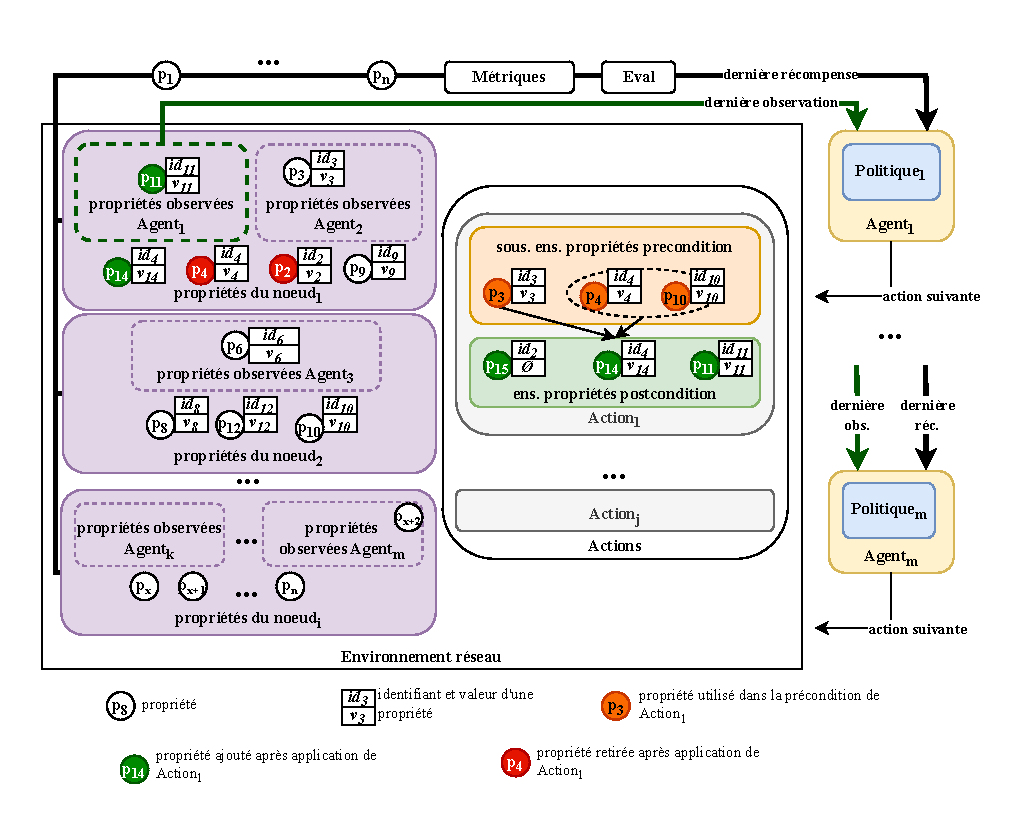
\includegraphics[trim=0.7cm 0.6cm 0.7cm 1cm, clip,width=1\textwidth]{figures/model_example_illustration.pdf}
  \caption{Illustrative view of the simulation model}
  \label{fig:model_example_illustration}
\end{figure*}

\noindent
The \acn{Dec-POMDP} model expresses the state as the set of node properties. Actions are defined by pre/post-conditions on these properties. Transitions and observations are conditioned by these properties, and rewards are calculated from metrics on the state.

\subsubsection{Dec-POMDP formal modeling}

We define the elements related to the properties of the nodes, agents, and actions of the following environment:

\begin{itemize}

\item $Ag = \{ag_1,..,ag_{|Ag|}\}$: set of agents (cyber attackers and cyber defenders).
% \begin{itemize}
% \item With $Attackers \subseteq Ag$: the set of attacking agents
% \item With $Defenders \subseteq Ag$: the set of defending agents
% \end{itemize}

\item We call the pair $p = (id_{j}, v_{j})$ with $id_j \in {ID}$ and $v_j \in V$ a property.
\begin{itemize}
\item $\acn{ID}$: the set of property identifiers indicating how properties are organized in a non-flat data structure (such as $PC1.processes.agents.agent1$). These property identifiers can be used for a file path, the type of operating system used in a node, a command line used by an agent\dots
\item $V$: Set of property values. These may include the contents of a file, a complete description of the operating system, the result of a command line\dots
% \item $Values: \acn{ID} \rightarrow \mathcal{P}(V) = \{(id_{j}, V_{j}) \: | \: id_j \in {ID},$ $V_j \in \mathcal {P}(V)\}$: a bijection associating a property identifier with the set of different values with which it can be associated. For example, the identifier $ls\_command\_output$ can be associated with the following values $\{file.txt,\{file.txt,passwd.txt\}\}$
\end {itemize}

\item $P_{j} = \{ p_1, .., p_{|P_{j}|} \}$: the set of properties $p_{l}$ (with $l \in \{1,..,|P_{j}|\}$) of node $j$ ($j \in \mathbb{N} $). For example, these properties may include certain identifiers of running processes, the list of files in a folder, the type of operating system with a description, specific knowledge of an agent, etc.
\begin{itemize}
\item $P = P_1 \cup P_2 .. \cup P_{|P|} $: Set of all node properties.
\end {itemize}

\item $Obs: \mathcal{P}(P) \times Ag \rightarrow \mathcal{P}(P_{Ag}), P_{Ag} \subset P$: Relation that associates the properties of nodes and an agent with the subset of properties observed by the agent.



\item $Action: P_{pre} \rightarrow P_{post}$: Relation that associates a subset of properties implicit in an equivalent conjunctive Boolean precondition ($P_{pre} \subset \mathcal{P}(P)$) with a subset of all properties of the postcondition ($P_{post} \in \mathcal{P} (P)$). For example, the properties $p_1 = (agent\_X\_privilege\_level, \allowbreak root)$, $p_2 = (agent\_X\_acce\-\allowbreak ssed\_text\_editor, \allowbreak Vim)$ and $p_3 = (agent\_X\_bashrc\_known\_filepath, /home/user/ .bashrc)$ can form a precondition ($p_1 \land p_2 \land p_3$) for associating a new set of properties containing $p4 = (bashrc_file_modified_by_X_agent, \top)$. Two subsets of preconditions can be associated with the same subset of postconditions to model a Boolean disjunction.

\item $Metrics: \mathcal{P}(P) \times A \rightarrow \mathbb{R}^{n}$: gives metrics associated with a set of properties and a joint action. For example, the number of nodes still active, lateral movements, etc.

\end {itemize}


Using the formal description of a \acn{Dec-POMDP}~\cite{Oliehoek2016}, we propose the following pre-specialized \acn{Dec-POMDP} model:

\begin{itemize}
  \item $S = \{s_1, ..s_{|S|}\}, s_{i} \subseteq P \: and \: 1 \le i \le |S|$: The state space as sets of possible properties.

  \item $A_{i} = \{a_{i}^{1},..,a_{i}^{|A_{i}|}\}, a_{i}^j \in Action \: and \: 1 \le j \le |A_i|$: the set of possible actions for agent $i$.

  \item $T$: Set of conditional transition probabilities between states
        \begin{itemize}
          \item With $T(s,a,s') = \probP(s'|s,a)$, the relation that associates the probability of going from state $s \in S$ to state $s' \in S$ knowing that we have played $a = (P^a_{pre} \times P^a_{post}) \in A$ with $P^a_{pre} \subset \mathcal{P}(P)$ and $P^a_{post} \in \mathcal{P} (P)$
          \item With $\probP(s'|s,a) = 0$ if $s$ does not satisfy the precondition of $a$ (i.e., $\exists \: P_{pre_s}^{a} \in P_{pre}^{a} \: | \: P_{pre_s}^{a} \not\in \mathcal{P}(s)$).
          \item With $s' = (s - \{p_l= (id_l, v_l) | p_l is in s and id_l is in {id_k | (id_k, v_k) is in P^a_{post} and v_k is not nothing}}) \cup P^a_{post}$
        \end{itemize}



  \item $R : S \times A \rightarrow \mathbb{R}^2 = Eval \circ Metrics$: The reward function that takes a state and an action and associates a performance indicator (using the state metrics) for attackers and defenders.
        \begin{itemize}
          \item With $Eval : \mathbb{R}^{n} \rightarrow \mathbb{R}^2$, associates a metric vector with a reward for cyber attackers and cyber defenders.
        \end{itemize}



  \item $\Omega_{i} \subset Range(Obs | \{ (s, ag_i) | s \in S \: and \: ag_i \in Ag \}) \subset P$: set of observable properties for agent $ag_i$. For example, the content of a file, the output of a command log, the result of a port scan, etc.
        \begin{itemize}
          \item $\Omega = \Omega_1 \cup \Omega_2 .. \cup \Omega_{|Ag|} = Range(Obs)$: Set of all observable properties for all agents.
        \end{itemize}

  \item $O$: Set of conditional observation probabilities.
        \begin{itemize}
          \item With $O(s',a,o) = \probP(o|s',a)$, the relation that associates the probability of observing an observation $o \subset \Omega$ from the state $s' \in S$ induced by $a \in A$
          \item With $\probP (o|s',a) = 0$ if the state $s' \in S$ does not contain the properties of $o \subset \Omega$ (i.e., $o \not\in \mathcal{P}(s')$). For example, an agent performs the action $x\_reads\_a\_log\ _file$, which gives rise to a new state whose property belonging to agent x's knowledge is $(log\_file\_content\_known\_by\_x, \allowbreak abc)$. This property will therefore be included in the observations returned to agent x.
        \end{itemize}

\end{itemize}


\subsubsection {Integration of attack/defense scenarios}

\noindent
From a raw perspective, the modeling of the proposed pre-specialized Dec-POMDP relies on actions to simulate how a real networked system would react, including vulnerabilities and countermeasures applied by cyberattackers and cyberdefenders.

A first challenge is to construct an attack/defense scenario representative of a networked system with vulnerabilities in order to enable an attack by linking only available information (such as known tactics, techniques, and procedures from MITRE ATT&CK) and selecting relevant defense countermeasures (from MITRE ATT&CK mitigation measures) and a deployment environment. A second challenge is to establish the actions corresponding to the attack/defense scenario. As actions modify the properties of the environment, they also have an impact on the space of possible states and the transitions between them.
Furthermore, when considering a low level of abstraction, many simple actions can accurately describe the changes made to the network. However, this increases the number of actions, and even more so the number of states, as these are combinations of the effects of the actions.

These challenges are directly related to the issues studied concerning the automated generation of attack graphs using available databases, possibly integrating artificial intelligence techniques, as in ~\cite{GFalco2018}. We do not intend to dwell further on these issues, as they are beyond the scope of this work.

This model, illustrated in \autoref{fig:model_example_illustration}, allows us to generate a faithful multi-agent simulator, where each action and observation is explicitly defined, facilitating extension to various cyber defense contexts.

\

\noindent
\textbf{MITRE ATT&CK integration approach}: We suggest a high-level manual approach that we used to integrate MITRE ATT&CK information in the form of an AD tree, as it formalizes the actions to be performed in a scenario and their interactions with the environment. It aims to help establish the attack/defense actions that will ultimately be integrated into the simulator:
%
% \begin{enumerate*}[label=\arabic*),itemjoin={;\quad}]
\begin{itemize}
  \item For a given advanced persistent threat (APT), we identified the relevant MITRE ATT&CK tactics, techniques, and procedures that seemed relevant to a networked system

  \item We produced a description linking the identified tactics to each other and to the associated techniques, sub-techniques, and procedures in order to create a scenario describing how the APT group could attack the networked system. This step defines the network topology with its main properties
        (such as an enterprise network consisting of several dedicated database servers communicating via FTP and HTTP, etc.)

  \item We created an AD tree structure as proposed in ~\cite {BKordy2010} with tactics as the main action objectives and techniques, sub-techniques, and procedures in the lower part of the tree. We ensured that there were multiple paths to achieve the same main action objective. We took care to define each attack action with prerequisites and postconditions based on the properties of the environment.

  \item We extracted the MITRE ATT&CK techniques/sub-techniques related to detection and mitigation measures, which we added to the AD tree to enrich the attack nodes. We made sure to define each defense action with preconditions and postconditions based on properties in the environment.

  \item We also listed and defined the main deployment-specific environmental actions from the previous description of the deployment environment or extended attack/defense actions that are common to cyber defenders and cyber attackers. This step results in a more realistic environment, providing a representative number of plausible actions that an agent can choose from in many systems.
        These common actions could include at least:
        \begin{enumerate*}[label=\arabic*),itemjoin={;\quad}]
          \item Reading and writing files
          \item Creating, deleting, copying, moving, renaming, modifying file/folder properties.
          \item Accessing a folder, accessing the parent folder
          \item Selecting a file/folder to apply further actions to
          \item Executing a binary file
          \item Using a network protocol (such as HTTP, FTP, SSH, etc.).
          \item Other interactions with basic command lines related to system monitoring or control.
        \end{enumerate*}
        Next, the associated environmental properties should describe a file system, a terminal interface, a port with rules, operating system parameter properties, etc.
\end{itemize}

\section{Description and implementation in the activity}
% Present the generic algorithm for the modeling activity (inputs → outputs).
% Include the pseudo-code/algorithm in LaTeX environment as in the previous chapter.

\autoref{alg:modeling} describes the general flow of the modeling activity.
Each step is explained below in order to clarify its objectives and role in the construction of the final model.


\begin{algorithm}[h!]
  \caption{Algorithmic view of the modeling activity}
  \label{alg:modeling}
  \DontPrintSemicolon

  \KwIn{
  Initial environment $\mathcal{E}$,
  joint histories $\mathcal{D}_{H^j}$~;
  informal objective $\mathcal{G}_{\text{inf}}$~;
  discount factor $\gamma$~;
  action space $A$~;
  observation space $\Omega$
  }
  \KwOut{the simulated environment $d \in D \cup OD$}

  \vspace{0.5em}
  \tcp{1. Manual formalization of component functions}
  $(R^j_H, S^j_H, \texttt{Render}^j_H) \gets \texttt{manual\_formalize}(\mathcal{G}_{\text{inf}}, \mathcal{E}, A, \Omega)$ \;

  \vspace {0.5em}
  \If{\textit{user wants manual modeling}}{
    \Return{$(S,\{A_i\},T,R,\{\Omega_i\},O,\gamma) \gets \texttt{manual\_model}(\mathcal{G}_{\text{inf}}, \mathcal{E}, A, \Omega)$} \;
  }

  \vspace{0.5em}
  \tcp{2. Train autoencoders for observations}
  Extract observations $\Omega^j = \{\omega^j_t\}$ from histories $\mathcal{D}_{H^j}$ \;
  Train an autoencoder $(Enc, Dec)$ on $\Omega^j$ by minimizing the reconstruction error \;

  \vspace{0.5em}
  \tcp{3. Encode observations in histories}
  For each history $h^j = (\omega_t^j, a_t^j) \in \mathcal{D}_{H^j}$, encode each joint observation ${z}_t = Enc(\omega^j_t)$ to form the training set $\mathcal{B} = \{ \{(z_t, a^j_t, z_{t+1})\} = h_z^j, h_z^j \in \mathcal{D}_{H^j}\}$

  \vspace{0.5em}
  \tcp{4. Train the \acn{RLDM}}
  Initialize the \acn{RLDM} $\mathcal{T}^z = f(g)$

  \For{$h_z^j \in \mathcal{B}$}{
    \For{$(z_t, a^j_t, z_{t+1}) \in h^j$} {
      Train the \acn{RLDM} $\mathcal{T}^{z}$ by minimizing the mean squared error (\acparen{MSE}) between the prediction $\hat{z}_{t+1}$ and the actual value $z_{t+1}$.
    }
  }

  \vspace{0.5em}
  \tcp{5. Save the initial observations and train the JOPM}

  $\Omega^{\mathcal{T}^j}_0 \gets \{\omega^j_0\}$ extracted from the histories $\mathcal{D}_{H^j}$

  $\mathcal{T}^j(h_{t-1}, \omega_t, a_t) = \langle f(h_{t-1}, Enc(\omega^j_t), a^j_t), Dec(\mathcal{T}^{z}(h_{t-1}, Enc(\omega^j_t), a^j_t)) \rangle$ \;

  \vspace{0.5em}
  \tcp{6. Return the modeled elements}
  \Return{$(\mathcal{T}^j, \Omega^{\mathcal{T}^j}_0, R^j_H, S^j_H, \texttt{Render}^j_H)$}
\end{algorithm}



\paragraph{Step 1: Manual formalization of component functions.}
The first step consists of manually deriving three fundamental functions from informal descriptions of the overall objective and organizational constraints: the reward function $R^j_H$, the stop function $S^j_H$, and the optional rendering function $Render^j_H$.
This step requires the expertise of designers, who must transform high-level objectives (often expressed in natural language or in the form of business rules) into formal specifications that allow trajectories to be evaluated in the simulated environment.

\paragraph{Step 2: Training autoencoders for observations.}
Once the interaction histories have been collected, the joint observations $\ Omega^j$ are extracted.
As their dimension can be very high in a multi-agent context, they are compressed using autoencoders.
The encoder $Enc$ learns to transform observations into compact latent representations $z_t$, while the decoder $Dec$ reconstructs the original observations from these latents.
The goal is to minimize the reconstruction error, thus ensuring that the latents retain the essential information.

\paragraph{Step 3: Encoding observations in histories.}
The trained autoencoders are then used to transform the set of histories $\mathcal{D}_{H^j}$ into sequences of latent states.
Each observation $\omega_t^j$ is converted into a representation $z_t$, which allows a new training set $\mathcal{B}$ to be constructed, composed of triplets $(z_t, a_t^j, z_{t+1})$.
This encoding reduces the complexity of the input data and prepares the dynamic model for training.

\paragraph{Step 4: Training the recurrent latent dynamics model (RLDM).}
A recurrent latent dynamics model (\acn{RLDM}) is trained from the encoded set $\mathcal{B}$.
This model, denoted $\mathcal{T}^z$, learns to predict the evolution of latent states based on the hidden history $\tilde{h}_{t-1}$, the current encoded state $z_t$, and the joint action $a_t^j$.
Training is performed by minimizing the mean squared error between the prediction $\hat {z}_{t+1}$ and the actual latent $z_{t+1}$.
This learning mechanism makes it possible to capture the dynamics of the environment without direct access to the global state.

\paragraph{Step 5: Construction of the JOPM.}
Once the \acn{RLDM} has been trained, the initial observations $\Omega^{\mathcal {T}^j}_0$ are extracted from the histories and used to initialize the simulator.
The \acn{JOPM} $\mathcal{T}^j$ is then defined by combining the recurrent model $f$, the encoder $Enc$, and the decoder $Dec$.
Thus, for any given observation and action, $\mathcal{T}^j$ updates the hidden state and generates a predicted observation, thereby constituting a complete simulator of multi-agent interactions.

Step 6: Activity outputs.
Finally, the activity returns all modeled elements: the \acn{JOPM} $\mathcal{T}^j$, the set of initial observations $\Omega^{\mathcal{T}^j}_0$, the reward function $R^j_H$, the stop function $S^j_H$, and the optional rendering function $Render^j_H$.
These components constitute the core of the digital twin that will be used by the training, analysis, and transfer activities of the \acn{MAMAD} method.


\section{Summary}

\noindent
In summary, the modeling activity aims to provide a faithful and usable simulated environment for multi-agent training, combining explicit formalism (generic \acn{Dec-POMDP}) and automatic generation by multi-agent World Models. The outputs produced (the \acn{JOPM}, the set of initial joint observations, the reward function, the stopping function, and optionally the rendering function) form the basis of the digital twin used in the following steps. This approach ensures adaptability (through learning on real data), explainability (through the formal structure of the model), and reusability (thanks to the generic framework). However, the fidelity of the model depends on the quality and diversity of the historical data collected, and the computational cost of training autoencoders and \acn{RLDM} can be high for complex environments. Finally, the granularity of actions and the coverage of real dynamics remain inherent limitations of any simulation. The training activity will exploit this simulated model to optimize policies under organizational constraints, thus initiating the iterative cycle of the \acn{MAMAD} method.

\clearpage
\thispagestyle{empty}
\null
\newpage

\chapter{Training Policies Under Constraints}
\label{chap:training}

The \textit{training activity}\index{Training (TRN)} consists of optimizing the joint policies of agents in the simulated environment, taking into account organizational constraints.
It corresponds to the resolution phase of the design problem, exploiting the models produced by the modeling activity.

This activity is crucial because it links the criteria defined in \autoref{sec:criteria-evaluation} concerning performance (C2), adaptation (C3), explainability (C5), and control (C4), via the integration of explicit constraints into multi-agent learning.

\section*{Formal objectives}

The \textbf{inputs} of the training activity are:
\begin{itemize}
  \item the simulated environment $d \in D \cup OD$ produced by the modeling activity~;
        % \item the \acn{JOPM} $\mathcal{T}^j$ produced by modeling;
        % \item the initial observations $\Omega^{\mathcal{T}^j}_0$;
        % \item the history-based reward function $R^j_H$
        % \item the history-based stop function $S^j_H$;
        % \item the history-based rendering function $\texttt{Render}^j_H$ or empty $\emptyset$;
  \item the organizational specifications $\mathcal{MM}$ possibly derived from the organizational specifications of a previous refinement cycle;
  \item the informal organizational specifications $\mathcal{C}_{\text{inf}}$, particularly if this is the first refinement cycle.
        % \item the discount factor $\gamma$;
        % \item the observation space $\Omega$;
        % \item the action space $A$;
\end{itemize}

\noindent
The \textbf{expected output} is a trained joint policy $\pi^j = \{\pi^j_0, \pi^j_1, \dots, \pi^j_{|\mathcal{A}|}\}$.

\medskip
\noindent

\noindent The overall relationship can be expressed as:
\begin{displaymath}
  \hspace{3cm}\texttt{train}: (D \cup OD) \times \mathcal{MM} \times \mathcal{C}_{\text{inf}} \rightarrow \pi^j
\end{displaymath}

If $d \in OD$, then $d = (\Omega, A, \mathcal{T}^j, \Omega^{\mathcal{T}^j}_0, R^j_H, S^j_H, \texttt{Render}^j_H, \gamma)$, and if $d \in D$, then $d = (S,\{A_i\},T,R,\{\Omega_i\}, \allowbreak O,\gamma)$.

\section{Work mobilized and obstacles identified}

The activity of training policies under constraints is based on several families of work from the field of \acn{MARL} and the integration of organizational constraints.

On the \acn{MARL} side, classical methods such as independent learning, centralized learning with decentralized execution (\acn{CTDE}), or Q-learning and Policy Gradient algorithms and their multi-agent variants, form the basis for optimizing joint policies in simulated environments. These approaches are effective for maximizing collective performance, but they do not natively integrate explicit organizational constraints.

To address this shortcoming, several works from Safe \acn{RL} and Constrained MDPs (\acn{CMDP}) have been mobilized. Methods such as Constrained Policy Optimization (\acn{CPO}) or Deep Constrained Q-Learning (\acn{DCQL}) allow numerical constraints (safety, consumption, risk) into the learning process, but their expressiveness remains limited to local and numerical constraints, without taking into account complex organizational structures.

Reward shaping, shielding, or human feedback approaches offer flexible guidance mechanisms, allowing indirect influence on learned policies. However, they do not guarantee formal compliance with organizational constraints and remain difficult to interpret.

Finally, work on the integration of symbolic organizational models, such as $\mathcal{M}OISE^+$, offers a rich formalization of roles, missions, and collective relationships. However, their direct integration into the \acn{MARL} learning process remains a major obstacle, due to the difficulty of translating these specifications into operational constraints that can be exploited by learning algorithms.

In summary, the main obstacles identified are:
\begin{itemize}
  \item the lack of a unified framework for integrating symbolic organizational constraints into \acn {MARL} learning;
  \item the difficulty of ensuring compliance with these constraints while maintaining policy performance and adaptability;
  \item the lack of explainability and control over policies learned in complex and dynamic environments.
\end{itemize}

\section{Positioning and proposed contributions}

To overcome these obstacles, our approach proposes to combine the strengths of symbolic and connectionist frameworks by introducing the MOISE+MARL framework. This framework allows organizational specifications (roles, missions, permissions, obligations) to be explicitly integrated into the multi-agent learning process by translating them into constraint guides (action masking, reward shaping, goal guides) injected into \acn{MARL} algorithms.

Our main contribution consists of:
\begin{itemize}
  \item formalizing the integration of organizational specifications $\mathcal{M}OISE^+$ into \acn{MARL} via constraint guides, allowing the space of learned policies to be restricted or guided;
  \item proposing a new formalism, \acn{ODec -POMDP}, compatible with learned simulated environments (World Models), to enable training from observable data only;
  \item developing a generic training algorithm (see \autoref{alg:training_mamad}) that articulates these constraint guides with existing \acn{MARL} methods, thus ensuring compatibility between connectionist learning and compliance with organizational constraints;
  \item offer a certain degree of explainability and control over learned policies, thanks to the traceability of constraint guides and post-hoc analysis of emerging behaviors.
\end{itemize}

This positioning makes it possible to reconcile performance, adaptation, control, and explainability in the training of constrained multi-agent policies, paving the way for a more robust and transparent design of \acn{SMA} for critical environments such as cyber defense.

\subsection{MOISE+MARL to link $\mathcal{M} OISE^+$ with MARL}

\begin{figure}[h!]
\centering
\tikzset{every picture/.style={line width=0.75pt}} %set default line width to 0.75pt        

\begin{tikzpicture}[x=0.75pt,y=0.75pt,yscale=-1.2,xscale=1.4]
    %uncomment if require: \path (0,2584); %set diagram left start at 0, and has height of 2584

    %Straight Lines [id:da4973066741986565] 
    \draw [line width=1.5]    (118.21,2302.58) -- (203.1,2302) ;
    %Straight Lines [id:da14807114776731778] 
    \draw    (368.35,2272) -- (368.35,2294) -- (332.16,2294) ;
    \draw [shift={(330.16,2294)}, rotate = 360] [color={rgb, 255:red, 0; green, 0; blue, 0 }  ][line width=0.75]    (6.56,-1.97) .. controls (4.17,-0.84) and (1.99,-0.18) .. (0,0) .. controls (1.99,0.18) and (4.17,0.84) .. (6.56,1.97)   ;
    %Straight Lines [id:da16285043353898754] 
    \draw [line width=1.5]    (83.88,2398) -- (204.61,2398) ;
    %Straight Lines [id:da6299512000169913] 
    \draw    (169.94,2348) -- (204.61,2348) ;
    %Straight Lines [id:da64750232417664] 
    \draw    (84.65,2446) -- (383.15,2446) ;
    %Straight Lines [id:da35895220906699743] 
    \draw    (84.65,2230) -- (383,2230) ;
    %Straight Lines [id:da715014372569708] 
    \draw    (244.68,2262) -- (224.68,2262) -- (224.68,2408) ;
    \draw [shift={(224.68,2410)}, rotate = 270] [color={rgb, 255:red, 0; green, 0; blue, 0 }  ][line width=0.75]    (6.56,-1.97) .. controls (4.17,-0.84) and (1.99,-0.18) .. (0,0) .. controls (1.99,0.18) and (4.17,0.84) .. (6.56,1.97)   ;
    %Straight Lines [id:da71870438525014] 
    \draw    (251.96,2328) -- (286.51,2328) -- (286.51,2356) ;
    \draw [shift={(286.51,2358)}, rotate = 270] [color={rgb, 255:red, 0; green, 0; blue, 0 }  ][line width=0.75]    (6.56,-1.97) .. controls (4.17,-0.84) and (1.99,-0.18) .. (0,0) .. controls (1.99,0.18) and (4.17,0.84) .. (6.56,1.97)   ;
    %Straight Lines [id:da6006267784187092] 
    \draw [line width=0.75]  [dash pattern={on 0.84pt off 2.51pt}]  (252.87,2378) -- (252.87,2407) ;
    \draw [shift={(252.87,2410)}, rotate = 270] [fill={rgb, 255:red, 0; green, 0; blue, 0 }  ][line width=0.08]  [draw opacity=0] (5.36,-2.57) -- (0,0) -- (5.36,2.57) -- cycle    ;
    %Straight Lines [id:da8743336135156266] 
    \draw    (322.88,2304) -- (322.88,2316) ;
    \draw [shift={(322.88,2318)}, rotate = 270] [color={rgb, 255:red, 0; green, 0; blue, 0 }  ][line width=0.75]    (6.56,-1.97) .. controls (4.17,-0.84) and (1.99,-0.18) .. (0,0) .. controls (1.99,0.18) and (4.17,0.84) .. (6.56,1.97)   ;
    %Straight Lines [id:da14641229967966152] 
    \draw [line width=0.75]  [dash pattern={on 0.84pt off 2.51pt}]  (322.88,2378) -- (322.88,2407) ;
    \draw [shift={(322.88,2410)}, rotate = 270] [fill={rgb, 255:red, 0; green, 0; blue, 0 }  ][line width=0.08]  [draw opacity=0] (5.36,-2.57) -- (0,0) -- (5.36,2.57) -- cycle    ;
    %Straight Lines [id:da9260929933425808] 
    \draw [line width=0.75]  [dash pattern={on 0.84pt off 2.51pt}]  (286.51,2378) -- (286.51,2420) -- (312.61,2420) ;
    \draw [shift={(315.61,2420)}, rotate = 180] [fill={rgb, 255:red, 0; green, 0; blue, 0 }  ][line width=0.08]  [draw opacity=0] (5.36,-2.57) -- (0,0) -- (5.36,2.57) -- cycle    ;
    %Straight Lines [id:da3057006030233673] 
    \draw [line width=0.75]  [dash pattern={on 0.84pt off 2.51pt}]  (274,2449.7) -- (274,2457) ;
    \draw [shift={(274,2460)}, rotate = 270] [fill={rgb, 255:red, 0; green, 0; blue, 0 }  ][line width=0.08]  [draw opacity=0] (3.57,-1.72) -- (0,0) -- (3.57,1.72) -- cycle    ;
    %Straight Lines [id:da07288166228322246] 
    \draw    (342,2449.98) -- (342,2458) ;
    \draw [shift={(342,2460)}, rotate = 270] [color={rgb, 255:red, 0; green, 0; blue, 0 }  ][line width=0.75]    (6.56,-1.97) .. controls (4.17,-0.84) and (1.99,-0.18) .. (0,0) .. controls (1.99,0.18) and (4.17,0.84) .. (6.56,1.97)   ;
    %Shape: Ellipse [id:dp8508274348425935] 
    \draw   (95.09,2288.86) .. controls (95.09,2287.28) and (96.33,2286) .. (97.85,2286) .. controls (99.38,2286) and (100.62,2287.28) .. (100.62,2288.86) .. controls (100.62,2290.44) and (99.38,2291.71) .. (97.85,2291.71) .. controls (96.33,2291.71) and (95.09,2290.44) .. (95.09,2288.86) -- cycle ;
    %Straight Lines [id:da3825450168053828] 
    \draw    (97.85,2291.71) -- (97.85,2298.86) ;
    %Straight Lines [id:da521321206042058] 
    \draw    (97.85,2298.86) -- (93.71,2306) ;
    %Straight Lines [id:da055514206493922025] 
    \draw    (97.85,2298.86) -- (102,2306) ;
    %Straight Lines [id:da8996496708356774] 
    \draw    (102,2294.57) -- (93.71,2294.57) ;

    %Straight Lines [id:da31678488015771755] 
    \draw [line width=2.25]    (188,2454) -- (196.97,2454) ;
    \draw [shift={(201.97,2454)}, rotate = 180] [fill={rgb, 255:red, 0; green, 0; blue, 0 }  ][line width=0.08]  [draw opacity=0] (5.72,-2.75) -- (0,0) -- (5.72,2.75) -- cycle    ;
    %Shape: Ellipse [id:dp3927356466672782] 
    \draw   (238.88,2451.17) .. controls (238.88,2450.36) and (239.67,2449.7) .. (240.64,2449.7) .. controls (241.61,2449.7) and (242.4,2450.36) .. (242.4,2451.17) .. controls (242.4,2451.99) and (241.61,2452.65) .. (240.64,2452.65) .. controls (239.67,2452.65) and (238.88,2451.99) .. (238.88,2451.17) -- cycle ;
    %Straight Lines [id:da3365602555559104] 
    \draw    (240.64,2452.65) -- (240.64,2456.32) ;
    %Straight Lines [id:da7990875235744026] 
    \draw    (240.64,2456.32) -- (238,2460) ;
    %Straight Lines [id:da23945649338821617] 
    \draw    (240.64,2456.32) -- (243.28,2460) ;
    %Straight Lines [id:da11927353559661591] 
    \draw    (243.28,2454.12) -- (238,2454.12) ;

    %Straight Lines [id:da5816423191130675] 
    \draw    (251.96,2272) -- (252.85,2356) ;
    \draw [shift={(252.87,2358)}, rotate = 269.39] [color={rgb, 255:red, 0; green, 0; blue, 0 }  ][line width=0.75]    (6.56,-1.97) .. controls (4.17,-0.84) and (1.99,-0.18) .. (0,0) .. controls (1.99,0.18) and (4.17,0.84) .. (6.56,1.97)   ;
    %Straight Lines [id:da9310455126832857] 
    \draw    (321.97,2338) -- (321.97,2356) ;
    \draw [shift={(321.97,2358)}, rotate = 270] [color={rgb, 255:red, 0; green, 0; blue, 0 }  ][line width=0.75]    (6.56,-1.97) .. controls (4.17,-0.84) and (1.99,-0.18) .. (0,0) .. controls (1.99,0.18) and (4.17,0.84) .. (6.56,1.97)   ;
    %Shape: Rectangle [id:dp293492578719597] 
    \draw   (120,2453) .. controls (120,2451.34) and (121.34,2450) .. (123,2450) -- (127.72,2450) .. controls (129.37,2450) and (130.72,2451.34) .. (130.72,2453) -- (130.72,2457) .. controls (130.72,2458.66) and (129.37,2460) .. (127.72,2460) -- (123,2460) .. controls (121.34,2460) and (120,2458.66) .. (120,2457) -- cycle ;
    %Straight Lines [id:da33566712615128225] 
    \draw    (261.05,2262) -- (306,2262) ;
    \draw [shift={(308,2262)}, rotate = 180] [color={rgb, 255:red, 0; green, 0; blue, 0 }  ][line width=0.75]    (6.56,-1.97) .. controls (4.17,-0.84) and (1.99,-0.18) .. (0,0) .. controls (1.99,0.18) and (4.17,0.84) .. (6.56,1.97)   ;
    %Shape: Rectangle [id:dp28383270948937667] 
    \draw   (308,2236) -- (381.08,2236) -- (381.08,2276) -- (308,2276) -- cycle ;
    %Straight Lines [id:da18020989903965012] 
    \draw [line width=3]    (97.22,2282) -- (97.22,2270) ;
    \draw [shift={(97.22,2264)}, rotate = 90] [fill={rgb, 255:red, 0; green, 0; blue, 0 }  ][line width=0.08]  [draw opacity=0] (10.18,-4.89) -- (0,0) -- (10.18,4.89) -- cycle    ;
    %Straight Lines [id:da018421338049046554] 
    \draw [line width=3]    (97.22,2310) -- (97.11,2322.37) ;
    \draw [shift={(97.22,2328)}, rotate = 268.86] [fill={rgb, 255:red, 0; green, 0; blue, 0 }  ][line width=0.08]  [draw opacity=0] (10.18,-4.89) -- (0,0) -- (10.18,4.89) -- cycle    ;
    %Shape: Rectangle [id:dp7281037051878541] 
    \draw   (85.42,2450) -- (96.13,2450) -- (96.13,2460) -- (85.42,2460) -- cycle ;

    % Text Node
    \draw (362,2544.5) node  [font=\tiny] [align=left] {Role to constraint guide};
    % Text Node
    \draw (342,2524.5) node  [font=\tiny] [align=left] {Agents set};
    % Text Node
    \draw (342,2504.5) node  [font=\tiny] [align=left] {Actions set};
    % Text Node
    \draw (257,2584.5) node  [font=\tiny] [align=left] {Goal to constraint guide};
    % Text Node
    \draw (335,2484.5) node  [font=\tiny] [align=left] {Goals};
    % Text Node
    \draw (359,2564.5) node  [font=\tiny] [align=left] {Role to deontic specs.};
    % Text Node
    \draw (232,2564.5) node  [font=\tiny] [align=left] {Mission};
    % Text Node
    \draw (245,2544.5) node  [font=\tiny] [align=left] {Reward function};
    % Text Node
    \draw (248,2524.5) node  [font=\tiny] [align=left] {Goal-reward guide};
    % Text Node
    \draw (242,2504.5) node  [font=\tiny] [align=left] {Mission weight};
    % Text Node
    \draw (245,2484.5) node  [font=\tiny] [align=left] {Time constraints};
    % Text Node
    \draw (127,2584.5) node  [font=\tiny] [align=left] {Mission to goals};
    % Text Node
    \draw (129,2564.5) node  [font=\tiny] [align=left] {Role-reward guide};
    % Text Node
    \draw (128,2544.5) node  [font=\tiny] [align=left] {Role-action guide};
    % Text Node
    \draw (121,2524.5) node  [font=\tiny] [align=left] {Agent to role};
    % Text Node
    \draw (115,2504.5) node  [font=\tiny] [align=left] {Roles set};
    % Text Node
    \draw (122,2484.5) node  [font=\tiny] [align=left] {Deontic specs.};
    % Text Node
    \draw (310,2544) node  [font=\tiny] [align=left] {$\displaystyle \boldsymbol{rcg}$};
    % Text Node
    \draw (200,2504) node  [font=\tiny] [align=left] {$\displaystyle \mathcal{P}$};
    % Text Node
    \draw (200,2484) node  [font=\tiny] [align=left] {$\displaystyle \mathcal{T_{C}}$};
    % Text Node
    \draw (200,2564) node  [font=\tiny] [align=left] {$\displaystyle \mathcal{M}$};
    % Text Node
    \draw (77.5,2484) node  [font=\tiny] [align=left] {$\displaystyle \mathcal{DS}$};
    % Text Node
    \draw (310,2564) node  [font=\tiny] [align=left] {$\displaystyle \boldsymbol{rds}$};
    % Text Node
    \draw (310,2504) node  [font=\tiny] [align=left] {$\displaystyle \boldsymbol{A}$};
    % Text Node
    \draw (200,2544) node  [font=\tiny] [align=left] {$\displaystyle \boldsymbol{R}$};
    % Text Node
    \draw (310,2524) node  [font=\tiny] [align=left] {$\displaystyle \mathcal{A}$};
    % Text Node
    \draw (200,2524) node  [font=\tiny] [align=left] {$\displaystyle \boldsymbol{grg}$};
    % Text Node
    \draw (77.5,2564) node  [font=\tiny] [align=left] {$\displaystyle \boldsymbol{rrg}$};
    % Text Node
    \draw (77.5,2544) node  [font=\tiny] [align=left] {$\displaystyle \boldsymbol{rag}$};
    % Text Node
    \draw (200,2584) node  [font=\tiny] [align=left] {$\displaystyle \boldsymbol{gcg}$};
    % Text Node
    \draw (76.5,2524) node  [font=\tiny] [align=left] {$\displaystyle \boldsymbol{ar}$};
    % Text Node
    \draw (77,2584) node  [font=\tiny] [align=left] {$\displaystyle \boldsymbol{mo}$};
    % Text Node
    \draw (76.5,2504) node  [font=\tiny] [align=left] {$\displaystyle \mathcal{R}$};
    % Text Node
    \draw (310,2484) node  [font=\tiny] [align=left] {$\displaystyle \mathcal{G}$};


    % Text Node
    \draw  [fill={rgb, 255:red, 255; green, 255; blue, 255 }  ,fill opacity=1 ]  (241.82,2323) .. controls (241.82,2320.24) and (244.06,2318) .. (246.82,2318) -- (259.82,2318) .. controls (262.58,2318) and (264.82,2320.24) .. (264.82,2323) -- (264.82,2333) .. controls (264.82,2335.76) and (262.58,2338) .. (259.82,2338) -- (246.82,2338) .. controls (244.06,2338) and (241.82,2335.76) .. (241.82,2333) -- cycle  ;
    \draw (253.32,2328) node  [font=\scriptsize] [align=left] {$\displaystyle \boldsymbol{rcg}$};
    % Text Node
    \draw    (337,2252) -- (354,2252) -- (354,2272) -- (337,2272) -- cycle  ;
    \draw (345.5,2262) node  [font=\scriptsize] [align=left] {$\displaystyle \mathcal{Y}$};
    % Text Node
    \draw    (311,2252) -- (334,2252) -- (334,2272) -- (311,2272) -- cycle  ;
    \draw (322.5,2262) node  [font=\scriptsize] [align=left] {$\displaystyle \mathcal{T_{C}}$};
    % Text Node
    \draw    (357.39,2252) -- (378.39,2252) -- (378.39,2272) -- (357.39,2272) -- cycle  ;
    \draw (367.89,2262) node  [font=\scriptsize] [align=left] {$\displaystyle \mathcal{M}$};
    % Text Node
    \draw (347.43,2244) node  [font=\scriptsize] [align=left] {$\displaystyle \mathcal{DS}$};
    % Text Node
    \draw  [fill={rgb, 255:red, 255; green, 255; blue, 255 }  ,fill opacity=1 ]  (270,2257) .. controls (270,2254.24) and (272.24,2252) .. (275,2252) -- (288,2252) .. controls (290.76,2252) and (293,2254.24) .. (293,2257) -- (293,2267) .. controls (293,2269.76) and (290.76,2272) .. (288,2272) -- (275,2272) .. controls (272.24,2272) and (270,2269.76) .. (270,2267) -- cycle  ;
    \draw (281.5,2262) node  [font=\scriptsize] [align=left] {$\displaystyle \boldsymbol{rds}$};
    % Text Node
    \draw (158,2454.5) node  [font=\tiny] [align=left] {Relation name};
    % Text Node
    \draw (106.46,2454.5) node  [font=\tiny] [align=left] {Set};
    % Text Node
    \draw (255.47,2454.5) node  [font=\tiny] [align=left] {User};
    % Text Node
    \draw (216.32,2454.5) node  [font=\tiny] [align=left] {Define};
    % Text Node
    \draw (366.91,2454.5) node  [font=\tiny] [align=left] {Set relation};
    % Text Node
    \draw (306.61,2454.5) node  [font=\tiny] [align=left] {Impact on training};
    % Text Node
    \draw    (244.82,2410) -- (261.82,2410) -- (261.82,2430) -- (244.82,2430) -- cycle  ;
    \draw (253.32,2420) node  [font=\scriptsize] [align=left] {$\displaystyle \boldsymbol{A}$};
    % Text Node
    \draw    (314.84,2410) -- (331.84,2410) -- (331.84,2430) -- (314.84,2430) -- cycle  ;
    \draw (323.34,2420) node  [font=\scriptsize] [align=left] {$\displaystyle \boldsymbol{R}$};
    % Text Node
    \draw    (215.63,2410) -- (234.63,2410) -- (234.63,2430) -- (215.63,2430) -- cycle  ;
    \draw (225.13,2420) node  [font=\scriptsize] [align=left] {$\displaystyle \mathcal{A}$};
    % Text Node
    \draw  [fill={rgb, 255:red, 255; green, 255; blue, 255 }  ,fill opacity=1 ]  (309.97,2363) .. controls (309.97,2360.24) and (312.21,2358) .. (314.97,2358) -- (328.97,2358) .. controls (331.73,2358) and (333.97,2360.24) .. (333.97,2363) -- (333.97,2373) .. controls (333.97,2375.76) and (331.73,2378) .. (328.97,2378) -- (314.97,2378) .. controls (312.21,2378) and (309.97,2375.76) .. (309.97,2373) -- cycle  ;
    \draw (321.97,2368) node  [font=\scriptsize] [align=left] {$\displaystyle \boldsymbol{grg}$};
    % Text Node
    \draw    (274.56,2363) .. controls (274.56,2360.24) and (276.8,2358) .. (279.56,2358) -- (292.56,2358) .. controls (295.32,2358) and (297.56,2360.24) .. (297.56,2363) -- (297.56,2373) .. controls (297.56,2375.76) and (295.32,2378) .. (292.56,2378) -- (279.56,2378) .. controls (276.8,2378) and (274.56,2375.76) .. (274.56,2373) -- cycle  ;
    \draw (286.06,2368) node  [font=\scriptsize] [align=left] {$\displaystyle \boldsymbol{rrg}$};
    % Text Node
    \draw    (240.87,2363) .. controls (240.87,2360.24) and (243.11,2358) .. (245.87,2358) -- (259.87,2358) .. controls (262.63,2358) and (264.87,2360.24) .. (264.87,2363) -- (264.87,2373) .. controls (264.87,2375.76) and (262.63,2378) .. (259.87,2378) -- (245.87,2378) .. controls (243.11,2378) and (240.87,2375.76) .. (240.87,2373) -- cycle  ;
    \draw (252.87,2368) node  [font=\scriptsize] [align=left] {$\displaystyle \boldsymbol{rag}$};
    % Text Node
    \draw (156.15,2380.5) node  [font=\footnotesize] [align=left] {$\displaystyle  \begin{array}{{>{\displaystyle}l}}
                \ \ \boldsymbol{Constraint\ Guides} \\
                ( roles\ and\ goals\ logic)
            \end{array}$};
    % Text Node
    \draw  [fill={rgb, 255:red, 255; green, 255; blue, 255 }  ,fill opacity=1 ]  (309.93,2323) .. controls (309.93,2320.24) and (312.17,2318) .. (314.93,2318) -- (329.93,2318) .. controls (332.69,2318) and (334.93,2320.24) .. (334.93,2323) -- (334.93,2333) .. controls (334.93,2335.76) and (332.69,2338) .. (329.93,2338) -- (314.93,2338) .. controls (312.17,2338) and (309.93,2335.76) .. (309.93,2333) -- cycle  ;
    \draw (322.43,2328) node  [font=\scriptsize] [align=left] {$\displaystyle \boldsymbol{gcg}$};
    % Text Node
    \draw  [fill={rgb, 255:red, 255; green, 255; blue, 255 }  ,fill opacity=1 ]  (214.77,2323) .. controls (214.77,2320.24) and (217.01,2318) .. (219.77,2318) -- (227.77,2318) .. controls (230.53,2318) and (232.77,2320.24) .. (232.77,2323) -- (232.77,2333) .. controls (232.77,2335.76) and (230.53,2338) .. (227.77,2338) -- (219.77,2338) .. controls (217.01,2338) and (214.77,2335.76) .. (214.77,2333) -- cycle  ;
    \draw (223.77,2328) node  [font=\scriptsize] [align=left] {$\displaystyle \boldsymbol{ar}$};
    % Text Node
    \draw  [fill={rgb, 255:red, 255; green, 255; blue, 255 }  ,fill opacity=1 ]  (356.85,2289) .. controls (356.85,2286.24) and (359.08,2284) .. (361.85,2284) -- (374.85,2284) .. controls (377.61,2284) and (379.85,2286.24) .. (379.85,2289) -- (379.85,2299) .. controls (379.85,2301.76) and (377.61,2304) .. (374.85,2304) -- (361.85,2304) .. controls (359.08,2304) and (356.85,2301.76) .. (356.85,2299) -- cycle  ;
    \draw (368.35,2294) node  [font=\scriptsize] [align=left] {$\displaystyle \boldsymbol{mo}$};
    % Text Node
    \draw (127,2344.5) node  [font=\small] [align=left] {$\displaystyle  \begin{array}{{>{\displaystyle}l}}
                \mathbf{MOISE\ +MARL} \\
                \mathbf{Specs.\ Level}
            \end{array}$};
    % Text Node
    \draw (127,2422.5) node  [font=\small] [align=left] {$\displaystyle  \begin{array}{{>{\displaystyle}l}}
                \mathbf{MARL\ Level} \\
                \mathbf{(Dec-POMDP)}
            \end{array}$};
    % Text Node
    \draw    (243.91,2252) -- (260.91,2252) -- (260.91,2272) -- (243.91,2272) -- cycle  ;
    \draw (252.41,2262) node  [font=\scriptsize] [align=left] {$\displaystyle \mathcal{R}$};
    % Text Node
    \draw (182.64,2315) node  [font=\footnotesize] [align=left] {$\displaystyle \boldsymbol{Linkers}$};
    % Text Node
    \draw    (313.93,2284) -- (330.93,2284) -- (330.93,2304) -- (313.93,2304) -- cycle  ;
    \draw (322.43,2294) node  [font=\scriptsize] [align=left] {$\displaystyle \mathcal{G}$};
    % Text Node
    \draw (127,2261.5) node  [font=\small] [align=left] {$\displaystyle  \begin{array}{{>{\displaystyle}l}}
                \mathbf{{\displaystyle Org.\ Specs.\ Level}} \\
                {\displaystyle \ \ \ \ \ \ \ \ \ \ \ (\mathcal{M}\mathbf{OISE^+})}
            \end{array}$};


\end{tikzpicture}
\caption[Minimal view of the MOISE+MARL framework]{Minimal view of the MOISE+MARL framework: Users first define the specifications $\mathcal{M} OISE^+$ specifications, which include roles ($\mathcal{R}$) and missions ($\mathcal{M}$), both associated via $rds$. They then create MOISE+MARL specifications by first defining constraint guides such as $rag$ and $rrg$ to specify role logic, and $grg$ for goal logic. Linkers are then used to connect agents to roles via $ar$ and to link the logic of constraint guides to the defined $\mathcal{M}OISE^+$ specifications. Once these elements are configured, roles can be assigned to agents, and the \acn{MARL} framework is updated accordingly during learning.
}
\label{fig:mm_synthesis}
\end {figure}

\noindent MOISE+MARL\index{MOISE+MARL} introduces ways to control or guide the learning of agents in \acn{MARL}. Its main contribution lies in \textbf{Constraint Guides}, which are three new relations introduced to describe the logic of roles and objectives in the \acn{Dec-POMDP} formalism:
%
\begin{itemize}
  % \begin{enumerate*}[label={\roman*) },itemjoin={; \quad}]

  \item \textbf{Role Action Guide} \quad $rag: H \times \Omega \rightarrow \mathcal{P}(A \times \mathbb{R})$, a relation modeling a role as a set of rules which, for each pair consisting of a history $h \in H$ and an observation received by the agent $\omega \in \Omega$, associates expected actions $A \in \mathcal {P}(A) each associated with a hardness constraint $ch \in [0,1]$ ($ch = 1$ by default). By restricting the choice of the next action among those allowed, the agent is forced to adhere to the expected behavior of the role
  \item \textbf{Role reward guide} \quad $rrg: H \times \Omega \times A \to \mathbb{R} = \{r_m \text{ if } a \notin A_\omega \text{, } rag(h, \omega) \allowbreak = \allowbreak A_\omega \times \mathbb{R} \text{, } h \in H; \text{ else } 0\}$, the relation that models a role by adding a penalty $r_m$ to the overall reward if the last action chosen by the agent $a \in A$ is not allowed. This aims to encourage the agent to adhere to the expected behavior.
  \item \textbf{Objective reward guide} \quad $grg: H \rightarrow \mathbb{R}$, the relation that models an objective as a soft constraint adding a reward bonus $r_b \in \mathbb{R}$ if the agent's history $h \in H$ contains a subsequence characteristic of an objective $h_g \in H_g$, encouraging the agent to achieve it.
        % \end{enumerate*}
\end{itemize}

\noindent Finally, we introduce \textbf{Linkers} to link organizational specifications $\mathcal{M}OISE^+$ to constraint guides and agents:
%
\begin{itemize}
  % \begin{enumerate*}[label={\roman*) },itemjoin={; \quad}]

  \item \textbf{Agent to Role} \quad $ar: \mathcal{A} \to \mathcal{R}$, the bijective relation linking an agent to a role;
  \item \textbf{Role to Constraint Guide} \quad $rcg: \mathcal{R} \rightarrow rag \cup rrg$, the relation associating each role $\mathcal{M} OISE^+$ to a relation $rag$ or $rrg$, forcing/encouraging the agent to follow the actions expected for the role $\rho \in \mathcal{R}$;
  \item \textbf{Guide Objective to Constraint} \quad $gcg: \mathcal {G} \rightarrow grg$, the relation linking objectives to relations $grg$, representing objectives as rewards in \acn{MARL}.
        % \end{enumerate*}
\end{itemize}

\subsubsection*{Solving \acn{Dec-POMDP} with MOISE+MARL}

A MOISE+MARL model is defined by $\mathcal{MM} = \langle \mathcal{OS}, ar, rcg, gcg, rag, rrg, grg \rangle$.
Solving a \acn{Dec-POMDP} with $mm \in \mathcal{MM}$ consists of finding a joint policy $\pi^j = {\pi^j_0, \pi^j_1, \dots, \pi^j_{|\mathcal {A}|}}$ that maximizes the expected cumulative reward (or satisfies a minimum threshold), represented by the state-value function $V^{\pi^j}$. This value reflects the return of an initial state $s \in S$ when successive joint actions $a^j \in A^{|\mathcal{A}|}$ are applied under additional organizational constraints.
%
The definition of $V^{\pi^j}$ follows the sequential and cyclic agent execution scheme (mode \acn{AEC}) and is formalized in \hyperref[eq:single_value_function]{Definition 1}, incorporating role-based (in red) and mission-based (in blue) adaptations that influence both the action space and the reward.
\autoref{fig:mm_synthesis} illustrates how $\mathcal{M}OISE^+$ specifications are integrated into \acn{Dec-POMDP} resolution via the MOISE+MARL framework.


\begin{figure*}[h!]
  \label{eq:single_value_function}
  \raggedright
  \textbf{\textit{Definition 1} \quad State-Value function adapted to constraint guides in \acn{AEC}:}

  \begin {scriptsize}
  \vspace{-0.6cm}
  \begin{gather*}
    V^{\pi^j}(s_t) = \hspace{-0.75cm}
    %
    \sum_{\textcolor{red}{ \substack{a_{t} \in A \text{ if } rn() < ch_{t}, \\
          a_{t} \in A_{t} \text{ else}}
      }}{\hspace{-0.7cm} \pi_i(a_{t} | \omega_t)}
    %
    \sum_{s_{t+1} \in S}
    %
    {\hspace{-0.1cm} T(s_{t+1} | s_t, a_{t})
    \Bigl[R(s_t,a_{t},s_{t+1}) + \hspace{-0.1cm}
    \textcolor{blue}{ \sum_{m \in \mathcal{M}_i}{ \hspace{-0.1cm} v_m(t) \frac{grg_m(h_{t+1})}{1 - p + \epsilon} } }
    + } \\
    {\textcolor{red}{(1-ch_t) \times rrg(\omega_t,a_{t+1})} + V^{\pi^j_{i+1 \ mod \ n}}(s_{t+1})\Bigr]}
  \end{gather*}
  %
  \vspace{-0.5cm}
  \textcolor{red}{\[\text{ \ hspace{-0.1cm} With } rag(h_t, \omega_t) = A_{t} \times \mathbb{R} \text{, } \langle a_t, ch_{t} \rangle \in A_{t} \times \mathbb{R} \text{ ; } rn: \emptyset \to [0,1[ \text{, a uniform random function}\]}
  %
  \vspace{-0.6cm}
  \textcolor{blue}{
    \begin{gather*}
      \hspace{-0.001cm}
      \text{With } \omega_t = O(\omega_t | s_t, a_t); } h_t = \{h_0 = \langle \rangle, h_{t+1} = \langle h_t, \langle \omega_{t+1}, a_{t+1} \rangle \rangle \} \text { ; } \epsilon \in \mathbb{R}_{>0} \text{ ; } grg_m(h) =
    \end{gather*}
  }
  \vspace{-0.95cm}
  \textcolor{blue}{
    \begin{gather*}
      \hspace{-0.5cm} \sum_{\hspace{0.3cm}(grg_i,w_i) \in mo(m)} {\hspace{-0.9cm} w_i \times grg_i(h)}
      \text{ ; } v_m(t) = \{ 1 \text{ if } t \in t_c \text{ ; else } 0 \} \text{ ; } \mathcal{M}_i = \{m_j | \langle ar(i),m_j,t_c,p \rangle \in \mathcal{M}\}
    \end{gather*}
  }
  \vspace{-0.6cm}
  \end{scriptsize}

\end{figure*}

At each time step $t \in \mathbb{N}$ (starting from $t=0$), agent $i = t \bmod n$ is assigned the role $\rho_i = ar(i)$. For each temporally valid deontic specification $d_i = rds(\rho_i) = \langle tc_i, y_i, m_i \rangle$, the agent is authorized ($y_i = 0$) or obligated ($y_i = 1$) to engage in mission $m_i \in \mathcal{M}$, with objective $\mathcal {G}_{m_i} = mo(m_i)$ and $n \in \mathbb{N}$ agents.
%
By observing $\omega_t$, the agent selects an action from $A_t$ (actions expected by the role) with probability $ch_t$, or from $A$ otherwise. If $ch_t = 1$, the agent is strictly constrained by their role.
%
The selected action changes the system from $s_t$ to $s_{t+1}$, generates the observation $\omega_{t+1}$ and returns a reward consisting of:
i) bonuses for objectives achieved in valid missions (via objective reward guides), weighted by $\frac{1}{1 - p + \epsilon}$;
ii) penalties from the role reward guide, scaled by $ch_t$.
%
The process continues in state $s_{t+1}$ with agent $(i + 1) \bmod n$.

\subsubsection*{Facilitating the implementation of \textbf{Constraint Guides}}
\subsection{Facilitating the implementation of \textbf{Constraint Guides}}

Since roles, objectives, and missions are simple labels, their definition is implicit. However, implementing a \(rag\), \(rrg\), or \(grg\) relationship requires defining numerous histories, often redundant, making an extensional definition tedious and not very scalable. In addition, the logic of each \textbf{Constraint Guide} is based on the analysis of agent trajectories: for each observed history, it is necessary to decide whether it belongs to a set of expected histories and what consequences to draw from it (masking actions, adding penalties or reward bonuses). For example, \(rag\) restricts the available actions according to whether the current trajectory belongs to a set \(H_g\) and the new observation.

A first approach is to let the user define these guides using procedural logic (Python scripts or specific rules). In this case, the relation \(b_g: H \to \ {0,1\}\) formalizes the decision of whether a history belongs to a set \(H_g\). This solution is flexible because it can exploit all of the available context (spatial positions, internal states, past sequences). However, it remains costly to write and maintain, and often leads to very verbose definitions.

To overcome this limitation, we introduce Trajectory-based Patterns (TPs), inspired by Natural Language Processing. The idea is to provide a compact declarative formalism for expressing expected behaviors as temporal patterns. A TP \(p \in P\) thus corresponds to a pattern that intentionally captures a set of histories. Each observation or action is associated with a label \(l \in L\) (via \(l: \Omega \cup A \to L\)), which makes manipulation practical and independent of low-level details of the environment.
%
A TP \(p\) can be:
\begin{itemize}
  \item a \textbf{leaf sequence} \(s_l = \langle h, \{c_{min}, c_{max}\} \rangle\), where \(h \in H\) denotes an observation/action subsequence and \(\{c_{min}, c_{max}\}\) is the cardinality;
  \item a \textbf {node sequence} \(s_n = \langle \langle s_{l_1}, s_{l_2}, \dots \rangle, \{c_{min}, c_{max}\} \rangle\), combining several sequences into a hierarchical pattern.
\end{itemize}

\noindent
For example, the pattern
%
$p = ``[o_1,a_1,[o_2,a_2]\langle0,2\rangle]\langle1,*\rangle"$
%
reads as follows: a valid history must contain at least one occurrence of the pair \(\langle o_1,a_1\rangle\), followed by zero to two occurrences of \(\langle o_2,a_2\rangle\). This TP therefore captures an entire family of behaviors, without having to list all histories.
%
% The correspondence relationship is then defined by:
% \[
% b_g(h) = m(p_g,h), \quad \text{with } m: P \times H \to \{0,1\},
% \]
where \(m(p_g,h)\) indicates whether a history \(h \in H\) satisfies the pattern \(p_g \in P\).
%
The TP has two advantages:
\begin{enumerate*}[label={\roman*) },itemjoin={; \quad}]
  \item They allow for \textbf{compact} coding of behaviors that extend over time and are difficult to express otherwise.
  \item They facilitate \textbf{reuse}, since the same patterns can be shared between several roles or objectives.
\end{enumerate*}

\paragraph{Concrete example.} Consider the \textit{Overcooked-AI}~\cite{overcookedai} environment, where chef agents must collaborate by moving around a grid world and interacting with ingredients (onions) and instruments (pots, bowls) to make soup, which is shipped by interacting with the shipping area. Here, we want to recognize the following behavior: \textquote{an agent who holds an onion observes a pot and interacts with it to fill it}. This behavior can be expressed by the following TP:
\[
  p = [[\#any](*) , \; has_onion , \; [\#any](*) , \; see_pot , \; interact \;](1,1)
\]

\noindent
This TP can be used in constraint guides as shown in \autoref{tab:tp_guides_example} to encourage the agent to interact again to retrieve the soup, for example.

\begin{table}[h]
  \centering
  \caption{Example of guides applied to the TP ``fill a pot with an onion''.}
  \label{tab:tp_guides_example}
  \scriptsize
  \renewcommand{\arraystretch}{1.3}
  % \setlength{\tabcolsep}{10pt}
  \begin{tabular}{p{2cm}@{\hspace{20pt}}p{6cm}}
    \hline
    \textbf{Guide}                            & \textbf{Example rule}                                    \\
    \hline
    \textbf{RAG} (\textit{Role Action Guide}) & If the TP is satisfied, restrict possible actions~:
    \[
      rag(h,\omega) = \{\texttt{interact} \mapsto 1.0, \;\texttt{nothing} \mapsto 0.2\}
    \]
    The action \texttt{interact} is strongly favored.                                                    \\
    \hdashline
    \textbf{RRG} (\textit{Role Reward Guide}) & Add a role bonus when the expected action is performed~:
    \[
      rrg(h,\omega,a) =
      \begin
      {cases}
    +3                                        & \text{if } a = \text{interact}                           \\
    0                                         & \text{otherwise}
      \end{cases}
    \]                                                                                                   \\
    \hdashline
    \textbf{GRG} (\text{Goal Reward Guide})   & Grant a reward if the TP is detected/achieved:
    \[
      grg(h) =
      \begin{cases}
        +5 & \text{if the pot is full (TP recognized)} \\
        0  & \text{otherwise}
      \end{cases}
    \]                                                                                                   \\
    \hline
  \end{tabular}
\end{table}

Thus, instead of extensionally defining vast sets \(H_g\), the user describes a few symbolic patterns that capture the essence of the desired behaviors. MOISE+MARL then automatically applies these patterns to the guides (\(rag, rrg, grg\)), making their implementation more modular, scalable, and interpretable.

\subsection{Extension of MOISE+MARL to Multi-Agent \textit{World Models}}\label{sec:wm_extension}

\noindent In realistic environments, only transitions from the history of actions and observations received are available. To better represent this context, we introduce a new formalism called \textbf{\acn{Dec-POMDP} based on observations} (\acparen{ODec-POMDP}). An \acn{ODec-POMDP} $d \in OD$ (where $OD$ is the set of ODec-POMDPs) is defined as a quintuple~:
%
$d = (\mathcal{T}^j, \Omega^{\mathcal{T}^j}_0, R^j_H, S^j_H, \texttt{Render}^j_H)$
%
where~:
\begin{itemize}
  \item $\Omega$, the observation space~;
  \item $A$, the action space~;
  \item $\mathcal{T}^j$, the \acn{JOPM} estimating the next joint observation $\omega'$ from the history $\tilde{h} \in \mathcal{H}$, the current joint observation $\omega$ and the joint action $a$. The model also returns the updated recurrent hidden state $\tilde{h}'$~;
  \item $\Omega^{\mathcal{T}^j}_0$, the set of initial joint observations;
  \item $R^j_H~: H \times \Omega \times A \times \Omega \rightarrow \mathbb{R}$, the history-based reward function, calculating the reward from the previous history, the current observation and action, and the next observation;
  \item $S^j_H~: H \rightarrow \{0,1\}$ the history-based stop function that indicates whether the agent has reached the end of its episode or achieved its goal;
  \item $\texttt{Render}^j_H : H \rightarrow \emptyset$, an optional history-based visual rendering function;
  \item $\gamma \in [0, 1]$, the discount factor.
\end{itemize}

\noindent This formulation allows \acn{MARL} agents to operate solely on observable data, making the method compatible with learned simulated environments.

\subsubsection*{Solving an \acn{ODec-POMDP} with MOISE+MARL}

Solving an \acn{ODec-POMDP} with constraints $mm \in \mathcal{MM}$ consists of finding a joint policy $\pi^j = \{\pi^j_0, \pi^j_1, \dots, \pi^j_{|\mathcal{A}|}\ }$ that maximizes the expected cumulative reward (or satisfies a minimum threshold), via the observation-based value function $V_{\mathcal{T}^j}^{\pi^j}$. This function represents the expected return from an initial joint observation $\omega^j \in \Omega^{\mathcal{T}^j} _0$, a history $h^j$, and a hidden state $\tilde{h}$, by applying joint actions $a^j \in A^{|\mathcal{A}|}$ under organizational constraints $\mathcal{MM}$, and using $\mathcal{T}^j$ to approximate transitions.

The complete definition of $V_{\mathcal{T}^j}^{\pi^j}$ is given in \hyperref[eq:single_value_function_parallel]{Definition 2}, and incorporates role-based (in red) and mission-based (in blue) adaptations, which influence both the joint action space and the reward. \autoref{fig:mm_synthesis} illustrates how $\mathcal{M}OISE^+$ specifications are injected into the resolution of an \acn{ODec-POMDP} using the MOISE+MARL framework.

\medskip

\begin{figure*}[h!]
\label{eq:single_value_function_parallel}
\raggedright
\textbf{\textit{Definition 2} \quad Observation-Value function adapted to constraint guides in parallel mode:}

\begin{scriptsize}
\vspace{-0.6cm}
\begin{gather*}
  \hspace{-1cm}V^{\pi^j}(\tilde{h}_{t-1},h^j_{t-1},\hat{\omega}^j_t) = \hspace{-0.95cm}
  %
  \sum_{\textcolor{red}{ \substack{a^j_{t} \in A^j \text{ if } rn() < ch_{t}, \\
  a^j_{t} \in A^j_{t} \text{ else}}
  }}{\hspace{-0.9cm} \pi_i(a^j_{t} | \hat{\omega}^j_t)}
  %
  \hspace {-1.2cm}
  \sum_{\phantom{XXXX}(\tilde{h}_t,\hat{\omega}^j_{t+1}) \in \mathcal{H} \times \hat{\Omega}^j}
  %
  {\hspace{-1.2cm} \mathcal{T}^j(\langle \tilde{h}_t,\hat{\omega}^j_{t+1} \rangle | \tilde{h}_{t-1}, \hat{\omega}_t, a^j_ {t})
  \Bigl[R^j_H(h^j_{t-1},\hat{\omega}^j_t,a^j_t,\hat{\omega}^j_{t+1}) \hspace{-0.1cm} }
\end{gather*}
%
\vspace{-1cm}
\begin{gather*}
  \hspace{3cm}
  {+ \ \textcolor{blue}{grg^j_m(h^j_t)}
  +
  \textcolor{red}{(1-ch_t) \times rrg^j(\hat{\omega}^j_t,a^j_{t+1})} + V^{\pi^j}(\tilde{h}_{t}, h^j_t, \hat {\omega}^j_{t+1})\Bigr]}
\end{gather*}
%
\vspace{-0.15cm}
%
\[\hspace{-0.9cm}\text{With \ } \tilde{h}_{-1} = \mathbf{0} \text{ and } \tilde{\omega}^j_0 \in \Omega_0^{\mathcal{T}^j} \text{ ; } a^j_t = \langle a_{t,0}, a_{t,1} \dots a_{t,|\mathcal{A}|} \rangle \text{ ; } \omega^j_t = \langle \omega_{t,0}, \omega_{t,1} \dots \omega_{t,|\mathcal{A}|} \rangle \text{ ; }\]
%
\vspace{-0.25cm}
\[\hspace{-0.5cm} h^j_t = \langle h_{t,0}, h_{t,1} \dots h_{t,|\mathcal{A}|} \rangle = \langle \langle h_{t-1,i}, \omega_{t,i}, a_{t,i} \rangle \rangle_{i \in \mathcal{A}}\]
%
\vspace{-0.2cm}
\textcolor{red}{\[\hspace{-1cm}\text{ \hspace{-0.1cm} With } \langle rag_i, rrg_i \rangle = rcg(ar(i)); rn: \emptyset \to [0,1[, a uniform random function}
%
\vspace{-0.3cm}
\textcolor{red}{\[A^j_t \times \mathbf{R}^{|\mathcal{A}|} = rag^j(h^j_t, \tilde{\omega}^j_t) = \langle rag_i(h_{t,i}, \omega_{t,i}) \rangle_{i \in \mathcal{A}} \text{ ; } rrg^j(h^j_t, \tilde{\omega}^j_t, a^j_t) = \sum_{i \in \mathcal{A}}{rrg_i(h_{t,i}, \omega_{t,i}, a_{t,i})}\]}
%
\vspace{-0.75cm}
\textcolor{blue}{
  \begin{gather*}
    \hspace{-1cm} grg_m(h) = \hspace{-1cm} \sum_{\hspace{0.3cm}(grg_i,w_i) \in mo(m)} {\hspace{-1.1cm} w_i \times grg_i(h)}
    \text{ ; }
    grg^j_m(h^j_t) = \hspace{-0.1cm} \sum_{i \in \mathcal{A}}{\sum_{m \in \mathcal{M}_i}{ \hspace{-0.1cm} v_m(t) \frac{grg_m(h_{t,i})}{1 - p + \epsilon} }} \text{ ; } \epsilon \in \mathbb{R}_{>0} \text{ ; }
  \end{gather*}
}
\vspace{-0.9cm}
\textcolor{blue}{
  \begin{gather*}
    \hspace{-1cm}
    v_m(t) = \{ 1 \text{ if } t \in t_c \text{ ; else } 0 \} \text{ ; } \mathcal{M}_i = \{m_j | \langle ar(i),m_j,t_c,p \rangle \in \mathcal{M}\}
  \end{gather*}
}
\end {scriptsize}

\end{figure*}

\noindent In parallel mode, at each time step $t \in \mathbb{N}$ (starting at $t=0$), each agent $i \in \mathcal{A}$ is assigned a role $\rho_i = ar (i)$. For each temporally valid deontic specification $d_i = rds(\rho_i) = \langle tc_i, y_i, m_i \rangle$, the agent is either authorized ($y_i = 0$) or obligated ($y_i = 1$) to engage in mission $m_i \ in \mathcal{M}$, with set of objectives $\mathcal{G}_{m_i} = mo(m_i)$.

When agents observe $\tilde{\omega}_t^j$, they select their actions from $A_{i,t}$ (derived via role reward guides) with probability $ch_t$, or in $A_t$ otherwise. If $ch_t = 1$, agents are strictly constrained by their role.

Observation and state transitions are approximated via \acn {JOPM} $\mathcal{T}^j$ from the previous hidden state $\tilde{h}_{t-1}$, the joint observation $\omega^j_t$, and the joint action $a^j_t$. The reward function $R^j_H$ uses this same information, along with the next observation, to produce the reward. Bonuses or penalties are then added according to:
i) the achievement of valid objectives (via the objective reward guides, weighted by $\frac{1}{1 - p + \epsilon}$),
ii) role compliance (via the role reward guides, weighted by $1 - ch_t$).

Although not indicated, in practice the stop function $S^j_H$ is used instead of the discount factor to terminate the step loop. Most often, this stop function consists of returning true when a threshold number of steps has been reached.
%
Similarly, if the history-based rendering function $\texttt{Render}$ is provided, it is used to visualize each agent's observations. This function is used primarily for explainability and supervision purposes.


\section{Description and implementation in the activity}

\autoref{alg:training_mamad} describes the general course of the training activity.
Each step is detailed below.

\paragraph{Step 1: Formalization of constraints.}
If the specifications $\mathcal{MM}$ are not provided, they are derived manually from the informal constraints $\mathcal{C}_{\text{inf}}$.

\paragraph{Step 2: Initialization.}
Initialize the parameters of the joint policy $\pi^j$ and an experience buffer $\mathcal{B}$.

\paragraph {Step 3: Execute simulated episodes.}
For each episode, sample an initial observation $\omega_0^j \in \Omega^{\mathcal{T}^j}_0$, initialize the history $h_{-1}^j$ and the hidden state $\tilde{h}_{-1}$.

\paragraph{Step 4: Select actions under constraints.}
At each step $t$, calculate the set of allowed actions $A_t^j = rag^j(h^j_t,\omega_t^j)$.
The agent selects its action $a_t^j$ from $A_t^j$ with probability $ch_t$, otherwise from $A$.

\paragraph{Step 5: Transition and update of the JOPM.}
The transition $(\tilde{h}_t,\omega_{t+1}^j)$ is generated by $\mathcal{T}^j(\tilde{h}_{t-1},\omega_t^j,a_t^j)$.

\paragraph{Step 6: Calculation of rewards.}
The reward $r_t$ combines:
\begin{itemize}
  \item the base reward $R^j_H$,
  \item a bonus $grg^j(h^j_t)$ if objectives are achieved,
  \item a bonus/penalty $(1-ch_t)\times rrg^j(h^j_t,\omega_t^j,a_t^j)$ related to role compliance.
\end{itemize}

\paragraph{Step 7: Experience update and learning.}
Transitions are stored in $\mathcal{B}$, and the policy $\pi^j$ is optimized by any compatible \acn{MARL} algorithm (Q-learning, Policy Gradient, \acn{CTDE}, etc.).

\paragraph{Step 8: Output.}
At the end of the episodes, the activity returns the trained joint policy $\pi^j$.


\begin{algorithm}[h!]
  \caption{Algorithmic view of the training activity}
  \label{alg:training_mamad}
  \DontPrintSemicolon

  \KwIn{
  Simulated environment as \acn{Dec-POMDP} or \acn{ODec-POMDP} $d \in D \cup OD$~;
  Organizational specifications $\mathcal{MM}$;
  Informal design constraints $\mathcal{C}_{\text{inf}}$;
  }
  \KwOut{$\pi^j$: Trained joint policy}

  \vspace{0.3em}

  \If{$\mathcal{MM} = \emptyset$}{
    $\mathcal{MM} \gets \texttt{manual\_formalize}(\mathcal{C}_{\text{inf}})$ \tcp*{Manual formalization of org. specs.} \;
  }

  \tcp*[l]{If env. simulated manually, classical training}
  \If{$d \in D$}{
    \textit{train a joint policy $\pi^j$ via constrained MARL according to \hyperref[eq:single_value_function]{Definition 1}} \;
  }
  \Else{

  Initialize policy parameters $\pi^j$ and replay buffer $\mathcal{B}$ \;

  \ForEach{episode $e = 1 \dots N$}{
  Sample $\omega_0^j \sim \Omega_0^{\mathcal{T}^j}$, initialize $\tilde{h}_{-1} \gets \mathbf{0}$ \;
  Initialize history $h_{-1}^j \gets \emptyset$ \;

  \ForEach{step $t = 0 \dots T$}{
  Compute $A_t^j = rag^j(h^j_t, \omega^j_t)$ via role reward guides in $\mathcal{MM}$ \;
  \If{$rn() < ch_t$}{
    Select $a_t^j \sim \pi^j(\cdot | \omega_t^j)$ from the set $A_t^j$ (constrained) \;
  }
  \Else{
    Select $a_t^j \sim \pi^j(\cdot | \omega_t^j)$ from the set $A_t$ \;
  }

  $(\tilde{h}_t, \omega_{t+1}^j) \gets \mathcal{T}^j(\tilde{h}_{t-1}, \omega_t^j, a_t^j)$ \tcp*{JOPM prediction}

  $r_t \gets \gamma^t \times R_H^j(h^j_{t-1}, \omega_t^j, a_t^j, \omega_{t+1}^j)$ \tcp*{Base reward}

  $r_t \gets r_t + grg^j(h^j_t)$ \tcp*{Bonus via objective guides}

  $r_t \gets r_t + (1 - ch_t) \times rrg^j(h^j_t, \omega_t^j, a_t^j)$ \tcp* {Bonus/penalty via role guides}

  Add $(\omega_t^j, a_t^j, r_t, \omega_{t+1}^j)$ to $\mathcal{B}$ \;
  Update $h^j_t \gets \langle \langle h_{t-1,i}, \omega_{t,i}, a_{t,i} \rangle \rangle_{i \in \mathcal{A}}$ \;

  Train $\pi^j$ with mini-batches drawn from $\mathcal{B}$ using any \acn{MARL} method \;
  }
  }
  }

  \Return{$\pi^j$}
\end{algorithm}



\section{Conclusion}

In summary, the training activity produces optimized joint policies that integrate both explicit organizational constraints and dynamics learned via multi-agent World Models.
This approach reconciles performance and adaptation while offering a certain degree of control and explainability.

The main limitations identified concern:
\begin{itemize}
  \item the scalability of \acn{MARL}, which requires a large number of agents;
  \item the dependence on available data to learn an accurate \acn{JOPM};
  \item the trade-off between strict compliance with constraints and optimal performance.
\end{itemize}

These elements prepare for the \textbf{analysis activity}, which aims to evaluate and explain the trained policies.


\clearpage
\thispagestyle{empty}
\null
\newpage

\chapter{Analyzing emerging behaviors}
\label{chap:analyzing}

The \textit{analysis activity}\index{Analysis (ANL)} aims to evaluate and explain the joint policies learned. It provides an explanation of the behaviors observed in terms of roles, objectives, and missions. This activity plays a central role in explainability by linking the dynamics learned to interpretable organizational structures.


\section*{Formal objectives}


The \textbf{inputs} to the analysis activity are:
\begin{itemize}
  \item an \acn{ODec-POMDP} $d$ representing the learned simulated environment;
  \item a trained joint policy $\pi^j$;
  \item an initial organizational specification $\mathcal{MM}$ (optional);
  \item the test episode window $w_{\text{episodes}}$.
\end{itemize}

\noindent
The \textbf{expected outputs} are:
\begin{itemize}
  \item the set of inferred implicit specifications $\mathcal{MM}_{\text{inferred}}$;
  \item the organizational fit score $\texttt{org\_fit}$ on the last $w_{\text{episodes}}$ episodes;
  \item the average rewards $\overline{r}$ over the last $w_{\text{episodes}}$ episodes;
  \item the standard deviation of rewards $\sigma$ over the last $w_{\text{episodes}}$ episodes;
  \item the Boolean indicating whether the user wishes to continue the refinement cycles $\texttt{running\_refinement}$.
\end{itemize}

\noindent The overall relationship can be expressed as:
\[
  \hspace{1cm}(\mathcal{MM}_{\text{inferred}}, \texttt{org\_fit}, \overline{r}, \sigma, \texttt{running\_refinement}) \gets \texttt{analyze}(d, \pi^j, \mathcal{MM}, w_{\text{episodes}})
\]

\section{Related work and identified challenges}

The analysis of emerging behaviors is based on three main areas: post-hoc explainability in machine learning, multi-agent policy analysis, and organizational inference from trajectories.

Local explainability methods (\acn{SHAP}, \acn{LIME}, \acn{CAV}) explain individual decisions, but remain limited for the overall analysis of collective dynamics. Interpretable models (decision trees, concept extraction) offer a certain degree of readability, but struggle to capture large-scale organizational complexity.

Trajectory clustering or role inference approaches can identify collective specializations or missions, but often require manual configuration and remain disconnected from symbolic organizational models.

To date, no method automatically extracts complete organizational specifications (roles, missions, permissions, obligations) from trajectories, nor systematically links emerging behaviors to a symbolic framework such as $\mathcal{M}OISE^+$.

The main obstacles are:
\begin{itemize}
  \item the absence of a framework for quantitatively assessing organizational explainability;
  \item the lack of automation in the inference of organizational structures;
  \item the absence of a method for linking extracted structures to existing symbolic models.
\end{itemize}

These limitations motivate the development of the \acn{TEMM} and \acn{Auto-TEMM} methods to automate organizational inference, quantify organizational adequacy, and link emerging behaviors to formal specifications that can be exploited in the design loop.



\section{Positioning and proposed contributions}
The analysis activity is central to the \acn{MAMAD} method, as it links learned dynamics to interpretable organizational structures and quantitatively assesses their alignment.

\textbf{Definition~:} \textit{Organizational fit} is theorized as the measure of conformity between observed collective behaviors and expected organizational specifications (roles, objectives, missions, permissions, obligations). It is quantified by a global indicator (\textbf{\acn{OF}}), combining structural (\acn{SOF}) and functional (\acn{FOF}) consistency extracted from trajectories.

Our approach proposes:
\begin{itemize}
  \item a global quantitative measure of organizational fit \acn{OF};
  \item the automatic extraction of implicit organizational specifications from trajectories;
  \item a flexible method, usable in manual mode (\acn{TEMM}) for expert analysis, or automated mode (\acn{Auto-TEMM}).
\end{itemize}

\acn{TEMM} allows expert control and qualitative analysis, while \textbf{\acn{Auto-TEMM}} automates the analysis and optimizes hyperparameters for large-scale use.

The main contributions are:
\begin{itemize}
  \item the introduction of a robust indicator of organizational fit;
  \item the formalization of an organizational inference method adapted to multi-agents;
  \item the automation of analysis via \acn{Auto-TEMM};
  \item the integration of this analysis into the \acn{MAMAD} design loop.
        \ end{itemize}

        In summary, organizational adequacy makes it possible to objectively evaluate, compare, and refine emerging behaviors, ensuring that the \acn{SMA} produced are effective, explainable, and aligned with organizational requirements.

        \subsection{The TEMM method}
        \label{sec:TEMM_algorithm}

        The \acn{TEMM} method is part of the explainability component of the MOISE+MARL framework. It is based on the assumption that agent behaviors, despite apparent variability, exhibit regularities when they achieve comparable cumulative rewards. Thus, different behaviors can be interpreted as noisy variants of a limited number of latent strategies. According to the law of large numbers, averaging over a sufficient set of successful joint histories allows noise to be filtered out and typical strategies to be revealed.

        The method uses unsupervised learning techniques to infer organizational specifications from the observed trajectories of agents and to calculate the organizational fit (\acn{OF}) between emerging behaviors and expected roles, objectives, and missions. It consists of three parts.

        \paragraph{1) Roles and role inheritance}
        The trajectories $(\omega, a) \in \Omega \times A$ are grouped into clusters using distance metrics (e.g., \acparen{LCS}, Smith-Waterman~\cite{smith1981identification}), possibly after one-hot encoding of the actions.
        In this framework, a \textbf{role} $\rho$ is defined as a policy whose agents share an \acn{SP} in their histories.
        We define a \textbf{Parent Sequence} as the \textit{local consensus sequence} obtained from the \textit{optimal local alignment} of the transition sequences considered, in the sense of the Smith-Waterman algorithm~\cite{smith1981identification}.
        This sequence captures the \textquote{most representative pattern} shared between two (or more) agent sequences, ignoring noise and divergences at the beginning and end of the sequence.
        It is not necessarily the longest common subsequence.
        The notion of \textit{local consensus sequence} is understood here in the classical sense of bioinformatics, namely a sequence representing the majority symbols in an aligned region~\cite{meshConsensusSequence,sternke2020consensus,schneider1990sequence}.

        A role $\rho_2$ inherits from $\rho_1$ if $\acn{SP}(\rho_2) \subseteq \acn{SP}(\rho_1)$.
        Hierarchical clustering allows these \acn{SP} to be extracted and a hierarchy of roles to be constructed.
        For each cluster, a centroid of average transitions per time step is calculated. A selection procedure retains the most representative transitions, interpreted as \textbf{behavioral rules} associated with a role.
        Low representativeness leads to the inclusion of all transitions, at the risk of over-learning.
        The \textbf{\acn{SOF}} (structural organizational fit) is calculated as the normalized inverse of the overall variance in the transition clusters: low variance indicates high structural consistency.

        \paragraph{2) Objectives, plans, and missions}
        Observation trajectories are grouped into clusters using distance metrics or vector methods (e.g., K-means on trajectory embeddings). For each cluster, a centroid trajectory is calculated, associating each time step with an average observation.
        \textbf{Representativeness} is defined as the normalized inverse of the local variance per time step.
        A minimum representativeness threshold is applied to select salient observations, interpreted as \textbf{intermediate objectives} – important milestones towards the overall objective.
        If the minimum representativeness is high, only very frequent observations are retained, ensuring robustness and relevance.
        The \textbf{plans} are inferred as sub-sequences of transitions systematically leading to these objectives.
        A \textbf{mission} groups together one or more objectives pursued collectively by one or more agents.
        The \textbf{\acn{FOF}} (functional organizational fit) assesses the functional consistency of agents in achieving these intermediate objectives, calculated as the normalized inverse of the variance in the observation clusters.

        \paragraph{3) Permissions and obligations}
        Permissions and obligations are derived by analyzing whether agents fulfilling a role systematically (or exclusively) accomplish certain missions within given time constraints.
        An obligation implies exclusivity, while a permission implies optionality.

        \paragraph{Aggregation and interpretation}
        The \textbf{overall organizational fit} is obtained by aggregating the structural and functional scores.
        A high score indicates that the inferred specifications (roles, objectives, tasks) are representative of the behaviors actually learned.
        A low score suggests weak structuring or inconsistent behaviors.
        Although some clustering hyperparameters may require manual adjustment to ensure the robustness of role and objective extraction, \acn{TEMM} provides a methodical approach to analyzing emerging organizational behaviors and refining specifications accordingly.


        \subsection{Auto-TEMM: the extended TEMM method with hyperparameter optimization}

        A major problem encountered with \acn{TEMM} is the need to manually choose several hyperparameters (distance metrics, clustering thresholds, representativeness thresholds), which slows down the analysis process and limits its automation. Too low representativeness leads to overfitting, while too high representativeness limits constraints and slows down convergence.


        To overcome this difficulty, we propose a process of ‘hyperparameter optimization’ (HPO) consisting of a grid search on possible combinations, aiming to maximize organizational fit and minimize the number of clusters:

        \begin {itemize}
  \item (i) For observations and transitions, apply a joint search on distance metrics and clustering thresholds to minimize intra-cluster variance and the number of clusters~;
  \item (ii) Determine the minimum representativeness (structural and functional) to obtain concise and relevant objectives and roles. Decreasing this representativeness increases coverage but reduces the robustness of organizational constraints. A high value limits generalization, while too low a value leads to overfitting. This is illustrated in \autoref{fig:conv_time_repr}, where normalized convergence time is plotted against minimum representativeness. Fast convergence indicates strong and consistent organizational constraints, while slow convergence suggests weak or inconsistent constraints.
\end{itemize}

We adopt a compromise based on the \textbf{inflection point} of the convergence/time graph (see \autoref{fig:conv_time_repr}), choosing the highest representativeness that ensures a normalized convergence of 3.5%. This strategy yields useful, interpretable, and generalizable specifications without excessive complexity.

\begin{figure}[h!]
  \centering
  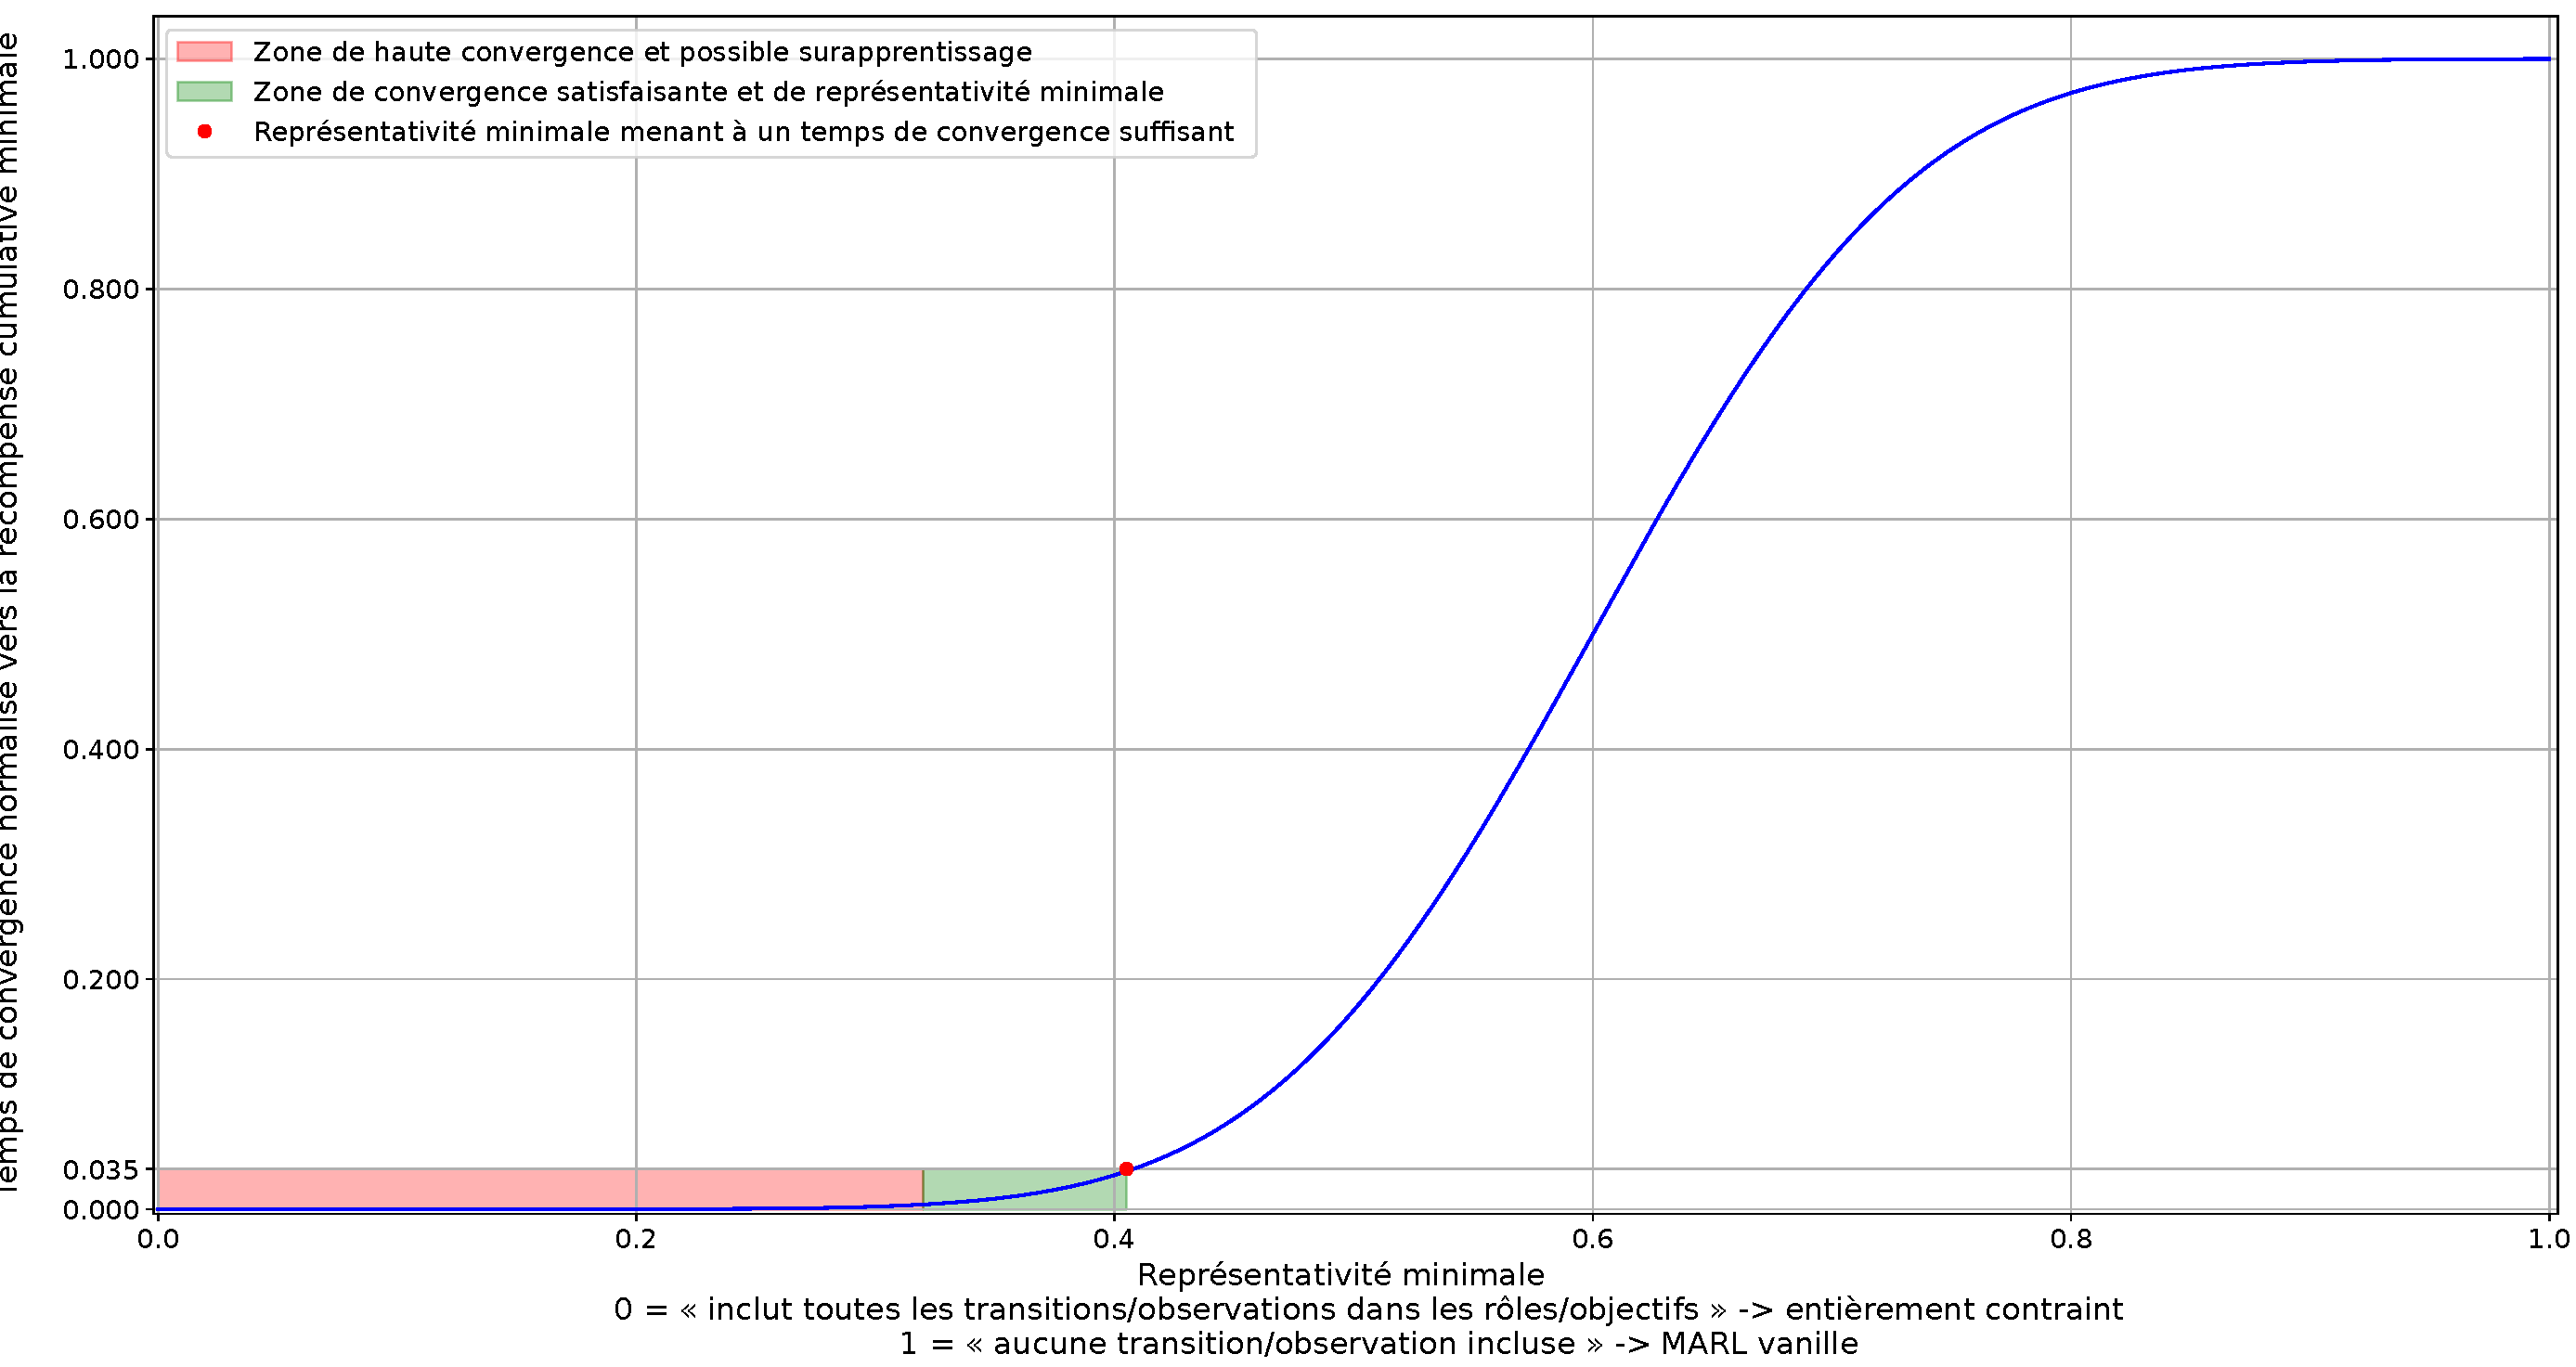
\includegraphics[trim=0cm 0cm 0cm 0cm, clip, width=1.\linewidth]{figures/convergence_time_relative_to_representativeness.pdf}
  \caption{Normalized convergence time as a function of minimum representativeness}
  \label {fig:conv_time_repr}
\end{figure}




\section{Description and implementation in the activity}

The \autoref{alg:auto_temm} formalizes the general course of the analysis activity.
Each step is detailed below in order to explain the mechanisms that allow us to infer an implicit organizational specification and calculate organizational adequacy.


\begin{algorithm}[h!]
  \caption{Algorithmic view of the analysis activity (Auto-TEMM)}
  \label{alg:auto_temm}
  \DontPrintSemicolon

  \KwIn{
    Joint policy $\pi^j$~;
    \acn{ODec-POMDP} $d$~;
    Initial specification $\mathcal{MM}$~;
    Normalized convergence threshold (default~: 3.5\%) $\eta$
  }

  \KwOut {
  Inferred organizational specification $\mathcal{MM}_{\text{inferred}}$;
  Organizational adequacy score $\acn{OF}$
  }

  \tcp*[l]{1. Trajectory collection}
  Generate individual histories $\mathcal{D}_{\text{trans}}$ from $d$ under $\pi^j$ \;
  $\mathcal{D}_{\text{obs}} \gets$ individual observation trajectories from $\mathcal{D}_{\text{full}}$ \;

  \tcp*[l]{2. \acn {HPO} on distance and clustering threshold}
  \For{$t \in \{obs, trans\}$}{
    \ForEach{distance metric $\delta_t$}{
      \ForEach{minimum cluster threshold $\tau_t$}{
        Apply clustering with $(\delta_t, \tau_t)$ \;
        Calculate $\sigma_{\text{obs}}, \sigma_{\text{trans} }, N_{\text{clusters}}$ \;
        Score $\gets \alpha (\sigma_{\text{obs}} + \sigma_{\text{trans}}) + \beta N_{\text{clusters}}$ \tcp*[l]{default~: $\alpha=0.4$, $\beta=0.6$}
        Retain $(\delta_t^*, \tau_t^*)$ with minimum Score \;
      }
    }
  }

  \tcp*[l]{3. Application of clustering with optimal \acn{HPO}}
  Clustering of observations: $\mathcal{D}_{\text{obs}} \rightarrow C_{obs}$ via $(\delta_{obs}^*, \tau_{obs}^*)$ \;
  Clustering transitions: $\mathcal{D}_{\text{trans}} \rightarrow C_{trans}$ via $(\delta_{trans}^*, \tau_{trans}^*)$ \;

  \tcp*[l]{4. \acn{HPO} on representativeness (convergence)}
  \For{$t \in \{obs, trans\}$}{
  \ForEach {representativeness $\rho_t$}{
  Infer $\mathcal{MM}_{\rho_t}$ from the clusters \;
  Initialize a policy $\pi^j_{\rho_t}$ \;
  Train $\pi^j_{\rho_t}$ on $(d, \mathcal{MM}_{\rho_t})$ until $R_{\min}$ is reached $ \;
    Record convergence time $c_{\rho_t}$ such that $ct_t(\rho_t) = c_{\rho_t}$ \;
    }

    \tcp*[l]{Select inflection point}
  $\rho_t^* \gets max(\{\rho_t \ | \ ct_t(\rho_t) < \eta \})$ \tcp*[r]{default $\eta = 3.5\%$}
    }

    \tcp*[l]{5. Inference of roles and objectives}
    Infer roles from $\mathcal{D}_{\text{trans}}, \delta^*, \tau^*, \rho^*$ \;
    Infer objectives from $\mathcal{D}_{\text{obs}}, \delta^*, \tau^*, \rho^*$ \;

    \tcp*[l] {6. Calculation of organizational fit}
    Calculate \acn{SOF} and \acn{FOF} from intra-cluster variances \;
  $\text{OF} \gets \frac{1}{2}(\text{SOF} + \text{FOF})$ \;

    \tcp*[l]{6.5. Manual refinement (optional)}
  $(\mathcal{MM}_{\text{inferred}} \times {0,1}) \gets \texttt{manual\_refine}(\mathcal{MM}_{\text{inferred}})$

    \Return{$\mathcal{MM}_{\text{inferred}}, \texttt{org\_fit}, \overline{r}, \sigma, \texttt{running\_refinement}$}
\end{algorithm}



\paragraph{Step 1: Collect trajectories.}
The first step is to execute the joint policy $\pi^j$ in the environment $d$ in order to generate complete histories of transitions $(\omega, a, \omega')$ on the $w_{\text{episodes}}$ of the validation window. This allows us to calculate the mean $\overline{r}$ and standard deviation $\sigma$ of the rewards over the collected episodes.
In addition, two datasets are extracted from these episodes:
\begin{itemize}
  \item $\mathcal{D}_{\text{trans}}$ containing the transition sequences $(\omega_t, a_t, \omega_{t+1})$, used for role inference;
  \item $\mathcal{D}_{\text{obs}}$ containing only the observation sequences $(\omega_t)$, used for objective and mission inference.
\end{itemize}

\paragraph{Step 2: Optimization of distances and clustering thresholds.}
To reduce variability between trajectories and identify recurring structures, the sets $\mathcal{D}_{\text{obs}}$ and $\mathcal{D}_{\text{trans}}$ are subjected to a clustering process.
Several distance metrics $\delta_t$ (e.g. \acn {LCS}, Smith-Waterman, vector distances) and clustering thresholds $\tau_t$.
Each combination $(\delta_t, \tau_t)$ is evaluated according to a weighted score:
\[
  \hspace{3.5cm}\text{Score} = \alpha (\sigma_{\text{obs}} + \sigma_{\text{trans}}) + \beta N_{\text{clusters}}
\]
where $\sigma$ denotes the intra-cluster variance and $N_{\text{clusters}}$ the total number of clusters.
The combination that minimizes this score is selected, ensuring a compromise between internal consistency and cluster compactness.

\paragraph{Step 3: Application of optimal clustering.}
Once the optimal hyperparameters $(\delta^*, \tau^*)$ have been determined, the trajectories are grouped together:
\begin{itemize}
  \item the transition clusters $C_{trans}$ are used to infer \textbf{roles} by extracting common sequences (\acn{CLS}) and associated behavioral rules;
  \item observation clusters $C_{obs}$ are used to identify \textbf{intermediate objectives} and associated plans.
\end{itemize}

\paragraph{Step 4: Search for optimal representativeness.}
The degree of representativeness $\rho_t$ sets the minimum threshold for a transition or observation to be retained as a characteristic of a role or objective.
A grid search is performed on different values of $\rho_t$.
For each $\rho_t$, a specification $\mathcal{MM}_{\rho_t}$ is inferred, then a new policy $\pi^j_{\rho_t}$ is retrained in $d$.
The convergence time $c_{\rho_t}$ to reach a minimum performance $R_{\min}$ is then recorded.
The optimal parameter $\rho_t^*$ is chosen as the highest representativeness guaranteeing convergence below the threshold $\eta$ (default 3.5%).

\paragraph{Step 5: Inference of roles and objectives. }
With $(\delta^*, \tau^*, \rho^*)$, we extract the roles $\mathcal{R}$, the intermediate objectives $\mathcal{G}$ and their hierarchical relationships (missions, role inheritance).
Permissions and obligations are deduced by observing the systematicity (obligations) or variability (permissions) of role-mission associations in the trajectories.

\paragraph{Step 6: Calculation of organizational fit.}
As with \acn{TEMM}, two partial indicators are calculated:
\begin{itemize}
  \item \textbf{\acn{SOF}} (structural organizational fit), measuring role consistency via the variance of intra-cluster transitions;
  \item the \textbf{\acn{FOF}} (functional organizational fit), measuring functional consistency in the achievement of intermediate objectives.
\end{itemize}
The overall indicator is obtained by aggregation:
$\text{OF} = \frac{1}{2}(\text{SOF} + \text{FOF})$

\paragraph{Step 6.5: Understanding and refining specifications.}
At this stage, the implicit organizational specifications $\mathcal{MM}_{\text{inferred}}$ are presented in the form of constraint guides, which are similar to rules linking observations to actions (RAG) or sets of observations (GRG). If desired, the user can examine and interpret these constraint guides in order to propose new organizational specifications that are more explicit and understandable. This step is optional, but it improves the robustness and interpretability of the organizational specifications. If the user does not modify the inferred specifications, they are retained and reused in the next refinement cycle to restrict the search space. If the user considers the results satisfactory, they can end the refinement cycles by setting the Boolean \texttt{running_refinement} to 0.

We include this optional step in the relation $\text{manual_refine}: \mathcal{MM}_{\text{inferred}} \rightarrow \mathcal{MM}_{\text{explicit}} \times {0,1}$, which takes the implicit specifications as input and returns explicit specifications (or the same ones if the user does not wish to modify them) as well as a Boolean indicating whether they wish to continue the refinement cycles.

\paragraph{Step 7: Activity outputs.}
The activity returns:
\begin{itemize}
  \item an implicit specification $\mathcal{MM}_{\text{inferred}}$ describing automatically inferred roles, missions, permissions, and obligations;
  \item the organizational fit score $\texttt{org\_fit}$ used to quantify the organizational quality of emerging behaviors;
  \item the mean $\overline{r}$ and standard deviation $\sigma$ of rewards over the analyzed episodes;
  \item a Boolean $\texttt{running\_refinement}$ indicating whether the user wishes to continue the refinement cycles.
\end{itemize}


\section {Conclusion}

In summary, the analysis activity establishes an objective link between the emerging behaviors of agents and the expected organizational structures. Thanks to the \acn{TEMM} method and its extension \acn{Auto-TEMM}, it becomes possible to automatically infer roles, objectives, and missions from trajectories, and to quantify their organizational adequacy using a robust indicator. This approach promotes explainability, traceability, and iterative refinement of organizational specifications, while providing evaluation tools to compare different policies or configurations. However, the quality of the analysis depends on the diversity of the trajectories collected and the choice of clustering hyperparameters, even if automation through joint optimization limits human intervention. This activity is therefore an essential pivot for the \acn{MAMAD} design loop, preparing for the transfer and continuous improvement of policies in the real environment.


\clearpage
\thispagestyle{empty}
\null
\newpage

\chapter{Transferring and supervising in the real environment}
\label{chap:transferring}

The \textit{transfer activity}\index{Transfer (TRF)} corresponds to the implementation and monitoring of joint policies in the real environment.
It plays a dual role: (i) ensuring the continuous execution of the most recent policy $\pi^j_{\text{latest}}$ in $\mathcal{E}$, guaranteeing the effective action of agents, and (ii) collecting new real trajectories $(\omega^j_t, a^j_t, \omega^j_{t+1})$ to enrich the database $\mathcal{D}_{H^j}$, enabling the updated simulated model and organizational specifications.

\section*{Formal objectives}

The \textbf{inputs} to the transfer activity are:
\begin{itemize}
  \item the most recent joint policy $\pi^j_{\text{latest}}$;
  \item the real environment $\mathcal{E}$;
  \item the accumulated trajectory database $\mathcal{D}_{H^j}$.
\end{itemize}

\noindent
The \textbf{expected outputs} are:
\begin{itemize}
  \item an enriched trajectory database $\mathcal{D}_{H^j}$;
  \item a $\texttt{need\_update}$ signal triggering the resumption of the design cycle.
\end{itemize}

The overall relationship can be expressed as:
\[
  \hspace{3cm}(\mathcal{D}_{H^j}, \texttt{need\_update}) \gets \texttt{transfer}(\pi^j_{\text{latest}}, \mathcal{E}, \mathcal{D}_{H^j}, \texttt{mode})
\]

\section{Related work and identified challenges}

Transfer and supervision in real-world environments rely on several approaches: policy transfer, domain adaptation (Sim2Real), online model calibration, and continuous supervision of \acplu{SMA}.

Robust Reinforcement Learning approaches~\cite{pinto2017robust} aim to make policies resistant to simulation/reality discrepancies, but do not include updating the simulated model after deployment. Domain adaptation and Sim2Real methods~\cite{tobin2017domain,ganin2016domain} reduce the simulation/reality gap through randomization or learning invariant representations, but their online adaptation remains limited. Dynamic calibration techniques~\cite{deisenroth2011pilco} update the simulated model based on real-world feedback, without explicitly considering the adaptation of multi-agent policies. Finally, manual synchronization remains common, but is not well suited to dynamic environments.

The main obstacles are:
\begin{itemize}
  \item the lack of a unified framework for the joint updating of the simulated model and the deployed policies;
  \item the difficulty of automatically detecting and correcting simulation/reality discrepancies;
  \item the lack of integrated mechanisms to ensure robustness and security during transfer;
  \item the need for continuous and automated supervision.
\end{itemize}

These limitations motivate the development of a methodological framework that ensures the joint adaptation of the digital twin and multi-agent policies, with automated supervision of the transfer.

\section{Positioning and proposed contributions}

The proposed approach introduces an \textbf{asynchronous and event-driven transfer framework} comprising:
\begin{itemize}
  \item a \textbf{Transfer Loop} (\texttt{Transfer Loop}) that ensures continuous policy execution and trajectory collection in a temporary buffer $\mathcal{B}$;
  \item an \textbf{Update Trigger} (\texttt{Update Trigger}) that adds trajectories to the database $\mathcal{D}_{H^j}$ and asynchronously activates modeling and training activities as soon as a threshold $\texttt{batch\_size}$ is reached.
\end{itemize}

This dual mechanism ensures the continuity of agent operation while keeping the design loop synchronized with real data.

\section{Description and implementation of the activity}

\autoref{alg:transferring} formalizes the operation of the transfer activity.
Each element is described below to clarify the mechanisms and their role in the design loop.


\vspace{-0.3em}
\begin{algorithm}[h!]
  \caption{Algorithmic view of the transfer activity}
  \label{alg:transferring}
  \DontPrintSemicolon
  \KwIn{
  Current policy $\pi^j_{\text{latest}}$,
  real environment $\mathcal{E}$,
  trajectory base $\mathcal{D}_{H^j}$,
  transfer mode $\texttt{mode} \in \{\texttt{DIRECT}, \texttt{REMOTE}\}$
  }
  \KwOut{Updated trajectory database $\mathcal{D}_{H^j}$, update signal $\texttt{need\_update}$}

  \vspace{0.3em}
  \SetKwProg{Transfer}{Procedure \normalfont TransferLoop}{}{}
  \Transfer{}{

  \While{the \acn{SMA} is active in the environment $\mathcal{E}$}{

  \uIf{$\texttt{mode} = \texttt{DIRECT}$}{
  \tcp*[l]{Each agent applies the policy locally}
  Agents observe locally $\omega^j_t$\;
  Local calculation $a^j_t \gets \pi^j_{\text{latest}}(\omega^j_t)$\;
  Local application of actions and update of state $\omega^j_{t+1}$\;
  Local storage $(\omega^j_t, a^j_t, \omega^j_{t+1})$ in an internal buffer\;
  Periodically: send local buffers to CybMASDE to update $\mathcal{D}_{H^j}$\;
  }
  \uElseIf{$\texttt{mode} = \texttt{REMOTE}$}{
  \tcp*[l]{The policy is executed by the Transferring process}
  $\omega^j_t \gets \texttt{observe}(\mathcal{E})$\;
  $a^j_t \gets \pi^j_{\text{latest}}(\omega^j_t)$\;
  $\omega^j_{t+1} \gets \texttt{apply}(\mathcal{E}, a^j_t)$\;
  Add $(\omega^j_t, a^j_t, \omega^j_{t+1})$ to temporary buffer $\mathcal{B}$\;
  }

  \tcp*[l]{Check if update is triggered}
  \If{$|\mathcal{B}| \geq \texttt{batch\_size}$} {
    Add $\mathcal{B}$ to $\mathcal{D}_{H^j}$ and empty $\mathcal{B}$ \;
    $\texttt{need\_update} \gets \texttt{True}$ \;
    \If{$\texttt{not running\_update} = \texttt{False}$}{
      \texttt{launch_update()} \tcp*[r]{Asynchronous call to the MTA process}
    }
  }
  }
  }
\end{algorithm}


\paragraph{Inputs and outputs.}
The activity receives the following inputs:
\begin{itemize}
  \item the most recent joint policy $\pi^j_{\text{latest}}$, produced during training;
  \item the real environment $\mathcal{E}$, representing the operational domain where the \acn{SMA} acts;
  \item the current trajectory database $\mathcal{D}_{H^j}$, enriched over the course of deployments.
\end{itemize}
At the output, it returns:
\begin{itemize}
  \item an updated trajectory base $\mathcal{D}_{H^j}$;
  \item a Boolean signal $\texttt{need\_update}$ indicating whether modeling and training activities should be restarted.
\end{itemize}

\paragraph{Transfer loop.}
The transfer loop runs as long as the \acn{SMA} is active in $\mathcal{E}$.
At each time step $t$:
\begin{enumerate}
  \item an observation $\omega^j_t$ is collected via the function $\texttt{observe}(\mathcal{E})$;
  \item the action $a^j_t$ is chosen by applying the policy $\pi^j_{\text{latest}}$ to the current observation;
  \item this action is executed in the environment via $\texttt{apply}(\mathcal{E}, a^j_t)$, producing the new observation $\omega^j_{t+1}$;
  \item the transition $(\omega^j_t, a^j_t, \omega^j_{t+1})$ is stored in a temporary buffer $\mathcal{B}$. \end{enumerate} \paragraph{Update trigger.} When the size of the buffer $\mathcal{B}$ exceeds a threshold $\texttt{batch\_size}$, the buffer $\mathcal{B}$ is flushed to disk.
  {B}$.
  \end{enumerate}

  \paragraph{Update trigger.}
  When the size of the buffer $\mathcal{B}$ exceeds a threshold $\texttt{batch\_size}$, the content is added to the trajectory database $\mathcal{D}_{H^j}$ and then the buffer is emptied.
  The $\texttt{need\_update}$ signal is then activated.
  If no update process is in progress (\texttt{not running\_update}), the \texttt{launch\_update()} procedure is triggered asynchronously to restart the modeling and training activities.

  \paragraph{Overall operation.}
  This scheme ensures three essential properties:
  \begin{itemize}
    \item \textbf{continuity of execution}: agents always operate with the latest available policy;
    \item \textbf{responsiveness}: real data is integrated as soon as a sufficient volume is collected;
    \item \textbf{automation}: updates are triggered without human intervention, while avoiding conflicts between parallel processes.
  \end{itemize}

  \paragraph{Formal elements.}
  %
  \begin{itemize}
  \item $\mathcal{B}$ denotes the temporary buffer (see \autoref{alg:transferring}),
  \item $\texttt{batch\_size}$ sets the granularity for triggering updates,
  \item $\texttt{launch\_update}()$ ensures synchronization with the other activities of the method.
\end {itemize}


\section{Summary}

In summary, the transfer activity ensures the continuous execution of the most recent policy and the automated collection of real trajectories to refine the model and retrain the policies.
%
Its advantages are:
\begin{itemize}
  \item automation of deployment and collection in a real environment;
  \item robust synchronization with other \acn{MAMAD} activities;
  \item continuous adaptation of agents to the environment.
\end{itemize}

Its limitations relate to the cost of supervision, the management of critical environments, and the optimal frequency of updates.
%
This activity proposes a \textbf{self-adaptive} method, alternating between simulated learning and real deployment to ensure the robustness of \acn{SMA} in a dynamic context.



\clearpage
\thispagestyle{empty}
\null
\newpage

\chapter*{Conclusion}
\addcontentsline{toc}{chapter}{\textbf{Conclusion}}

\noindent
This third part introduced the \textbf{\acn{MAMAD}} method as a concrete response to the limitations identified in current approaches to \acn{SMA} design. Based on an iterative cycle structured around four activities (\textit{Modeling}, \textit {Learning}, \textit{Analysis}, \textit{Transfer}), \acn{MAMAD} coherently articulates symbolic tools (organizational specifications) and \acn{MARL} to guide the design, training, and adaptation of intelligent agents in complex environments.

\medskip

\noindent
The method is based in particular on:
\begin{itemize}
  \item faithful modeling of environments based on empirical data,
  \item training constrained by organizational specifications integrated within the \textit{MOISE+MARL} framework,
  \item trajectory analysis to infer the emerging structures of the learned organization,
  \item and finally on a controlled transfer allowing iterative improvement of the \acn{SMA}.
\end{itemize}

\noindent
In the following section, we propose to experimentally validate this method through its concrete implementation in a dedicated tool, \acn{CybMASDE}\index{CybMASDE}, and its application to several representative environments. The objective is to demonstrate the ability of \acn{MAMAD} to automatically produce high-performance \acplu{SMA} that are explainable and compliant with organizational requirements in a variety of contexts.

\medskip

\noindent
In particular, we evaluate the method according to criteria of efficiency, automation, compliance with constraints, and explainability, while comparing its results to those of conventional approaches not guided by organizational models.

\bigskip

The \autoref{part:experimentation} therefore tests the \acn{MAMAD} method by analyzing its performance and relevance in relation to the constraints identified in different scenarios.